%% IFBTcc Latex Template Version
%% 	based on a fork of : RiSE Latex Template
%%
%% IFBthesis latex template for thesis and dissertations
%% https://github.com/IFBmodels/tcc
%%
%% (c) 2017 Rafael de Campos Passos (rcpassos@ieee.org)
%%
%% This document was initially based on RiSE Latex template, from Yguaratã
%% Cerqueira Cavalcanti
%%
%% GENERAL INSTRUCTIONS
%%
%% We strongly recommend you to compile your documents using pdflatex command.
%% It is also recommend use the texlipse plugin for Eclipse to edit your documents.
%%
%% Options for \documentclass command:
%%         * Idiom
%%           pt   - Portguese (default)
%%           en   - English
%%
%%         * Text type
%%           bsc  - B.Sc. Thesis
%%           msc  - M.Sc. Thesis (default)
%%           qual - PHD qualification (not tested yet)
%%           prop - PHD proposal (not tested yet)
%%           phd  - PHD thesis
%%
%%         * Media
%%           scr  - to eletronic version (PDF) / see the users guide
%%
%%         * Pagination
%%           oneside - unique face press
%%           twoside - two faces press
%%
%%		   * Line spacing
%%           singlespacing  - the same as using \linespread{1}
%%           onehalfspacing - the same as using \linespread{1.3}
%%           doublespacing  - the same as using \linespread{1.6}
%%
%% Reference commands. Use the following commands to make references in your
%% text:
%%          \figref  -- for Figure reference
%%          \tabref  -- for Table reference
%%          \eqnref  -- for equation reference
%%          \chapref -- for chapter reference
%%          \secref  -- for section reference
%%          \appref  -- for appendix reference
%%          \axiref  -- for axiom reference
%%          \conjref -- for conjecture reference
%%          \defref  -- for definition reference
%%          \lemref  -- for lemma reference
%%          \theoref -- for theorem reference
%%          \corref  -- for corollary reference
%%          \propref -- for proprosition reference
%%          \pgref   -- for page reference
%%
%%          Example: See \chapref{chap:introduction}. It will produce
%%                   'See Chapter 1', in case of English language.
%%
%% Citation commands:
%%          \citet (from natbib) -- To cite a reference as part of the narrative
%%          \citep (from natbib) -- To cite a reference between parenthesis
%%          citationblock environment -- To produce direct citation blocks according to the ABNT

\documentclass[pt,twoside,onehalfspacing,bsc]{ifbclass/ifbclass}
\usepackage[brazil]{babel}
\usepackage[utf8]{inputenc}
  \usepackage{graphicx}
  \usepackage{colortbl}
  \usepackage{color}
  \usepackage[table]{xcolor}
  \usepackage{microtype}
  \usepackage{bibentry}
  \usepackage{subfigure}
  \usepackage{multirow}
  \usepackage{rotating}
  \usepackage{booktabs}
  \usepackage{pdfpages}
  \usepackage{caption}
  \usepackage{lipsum}
  \usepackage{sectsty}
  \usepackage{tikz}
  \usepackage{amsmath}
  \usepackage{mathtools}%para teto e chão
  \usepackage{pdflscape}
  \usepackage{url}
  \usepackage[linesnumbered,lined,algoruled,vlined,longend]{algorithm2e}
  \usepackage{amssymb}% http://ctan.org/pkg/amssymb
  \usepackage{pifont}% http://ctan.org/pkg/pifont
  \newcommand{\cmark}{\ding{51}}%
  \newcommand{\xmark}{\ding{55}}%
  %% Set the language used in your code in the block above
  
  \DeclarePairedDelimiter{\ceil}{\lceil}{\rceil}
  \DeclarePairedDelimiter{\floor}{\lfloor}{\rfloor}
  \DeclareMathOperator*{\argmax}{arg\,max}
  \DeclareMathOperator*{\argmin}{arg\,min}
  
  \newcounter{examplecounter}
  \newenvironment{example}{
    \begin{quote}%
    \refstepcounter{examplecounter}%
    \textbf{Examplo \arabic{examplecounter}:}%
    \quad
  }
  {%
    \end{quote}%
  }


  \captionsetup[table]{position=top,justification=centering,width=.85\textwidth,labelfont=bf,font=footnotesize}
  \captionsetup[lstlisting]{position=top,justification=centering,width=.85\textwidth,labelfont=bf,font=footnotesize}
  \captionsetup[figure]{position=bottom,justification=centering,width=.85\textwidth,labelfont=bf,font=footnotesize}
  
  %% Chapter and (Sub)Section fonts must be same size as text (12)
  \sectionfont{\fontsize{12}{15}\selectfont}
  \subsectionfont{\fontsize{12}{15}\selectfont}
  \subsubsectionfont{\fontsize{12}{15}\selectfont}
  
  %% Change the following pdf author attribute name to your name.
  \usepackage[linkcolor=black,
              citecolor=black,
              urlcolor=black,
              colorlinks,
              pdfpagelabels,
              pdftitle={IFB tcc Template (ABNT)},
              pdfauthor={ifb ctag team},
              breaklinks=true]{hyperref}
  
  \address{BRASÍLIA}
  
  \universitypt{Instituto Federal de Educação, Ciência e Tecnologia de Brasília}
  \universityen{Federal Institute of Brasilia}
  
  \campus{Campus Taguatinga}
  
  \majorfieldpt{Bacharelado em Ciência da Computação}
  \majorfielden{Computer Science}
  
  \title{Uma proposta de Range min-Max tree k-ária para consultas sobre árvores sucintas}
  
  \date{2021}
  
  \author{Danyelle da Silva Oliveira Angelo}
  \adviser{Daniel Saad Nogueira Nunes}
  %\coadviser{Nome dompleto do co-orientador }
  
  % Macros (defines your own macros here, if needed)
  \def\x{\checkmark}
  %\let\lstlistoflistings\origlstoflistings
  
  \begin{document}
  
  \frontmatter
  
  \frontpage
  
  \presentationpage
  
  \begin{fichacatalografica}
    \FakeFichaCatalografica % Comment this line when you have the correct file
  %     \includepdf{fig_ficha_catalografica.pdf} % Uncomment this
  \end{fichacatalografica}
  
  \banca
  
  %\begin{dedicatory}
  %I dedicate this thesis to all my family, friends and professors who gave me the
  %necessary support to get here.
  %\end{dedicatory}
  
  %\acknowledgements
  %\lipsum[1-4]
  
  % \begin{epigraph}[]{Márcio de Deus}
  % When one finds a hard problem, the more complicated it is, the more one ought to work towards enlightening it's solution.
  % \end{epigraph}
  
  \resumo
  {\parindent0pt
    O desenvolvimento de novas aplicações em tempo real e o crescente aumento na produção de dados aliados à disparidade de desempenho entre processador 
e memória é um grande desafio para projetistas e desenvolvedores de software. Neste contexto, torna-se fundamental a utilização eficaz dos níveis superiores da hierarquia de memória, onde o tempo gasto para concluir uma  solicitação do processador é menor e a capacidade de armazenamento é  reduzida; essa utilização eficaz pode acontecer por intermédio das estruturas 
de dados sucintas, pois estas possibilitam a representação e operação sobre um conjunto de dados de maneira eficiente, ao mesmo tempo em que possibilitam  o seu gerenciamento em memórias mais rápidas e com capacidade de armazenamento menor. A range min-Max tree (rmM-tree) é um exemplo de sucesso dessas estruturas, construída na forma de uma árvore binária completa, a 
rmM-tree ocupa cerca de $n + O(\frac{n}{b} \log n)$ bits, e possibilita a realização de operações sobre os objetos em  tempo $O(\log n)$. Embora essa estrutura possua custo computacional teoricamente  satisfatório, devido ao seu baixo fator de ramificação, podem ocorrer um grande número de transferências de dados entre cache e memória RAM.  Este trabalho se concentra na proposta de uma estrutura range min-Max tree k-ária, visando um maior fator de ramificação, gerando em decorrência disso um melhor aproveitamento do príncipio de localidade espacial, contribuindo para a melhoria do desempenho das operações suportadas pela rmM-tree. 


\begin{keywords}
Estrutura de dados sucintas; Range min-Max tree; Árvores; Lacuna de desenvolvimento procesador-memória; Cache.
\end{keywords}
  }
  
  \abstract
  {\parindent0pt
    The development of new real-time applications and the crescent increase data production combined with the disparity in performance between  processor and memory is a major challenge for softwares designers and developers. In this context, it becomes essential to effectively use the higher levels of hierarchy of memory, where the time spent to complete a processor  request is less and the storage capacity is reduced;  the effective use of this hierarchy can take place through the succinct data structures, which allow the representation and operation on a set of data efficiently,  while allowing the management of this data in faster memories and with  less storage capacity. The Range min-Max tree (rmM-tree) is an example of the success of these structures, built in the form of a complete binary tree, the rmM-tree occupies  about $n + O (\frac {n} {b} \log n)$ bits, and makes it possible to perform operations in time $O(\log n)$.  Although this structure has theoretically satisfactory computational cost, due to its low branching factor, a large number of data transfers between  cache and RAM can occur. This work focuses on the proposal of a min-Max tree k-ary range, aiming a higher branching factor, as a result, generating a better use of the principle of spatial locality, contributing to the improvement of the performance of the operations supported by the rmM-tree.

\begin{keywords}
Succinct data structures; Range min-Max tree; Trees; Processor-memory development gap; Cache.
\end{keywords}
  }
  

  \tableofcontents
  
  \mainmatter
  
 \chapter{Introdução}
\label{chp:introduction}

A cada ano novas aplicações e dispositivos com formatos e recursos diversos são lançados no mercado, o crescimento de aplicações como as de transporte, dos serviços de streamings, a popularização de  dispostivos IoT, o crescimento dos datacenters e do serviço em nuvem vêm contribuindo fortemente para o aumento na produção de dados \citep{relatorio-idc}.

Especializada em computação em nuvem, a \citeauthor{domo-study} realiza anualmente uma análise da quantidade de informação produzida na internet  a cada \textit{minuto}. Abaixo vemos algumas das estatísticas relativas à esse estudo \citep{domo-study}:

\begin{itemize}
    \item 41.666.667 mensagens são enviadas através do aplicativo de mensagens WhatsApp;
    \item 479.452 pessoas interagem com conteúdos da plataforma Reddit;
    \item 208.333 pessoas participam de conferências no serviço de chamada Zoom, ao passo que o Microsoft Teams conecta cerca de 52.083 usuários por minuto;
    \item 147.000 uploads de fotos são feitos no Facebook e 150.000 mensagens são enviadas na mesma plataforma;
    \item 28 faixas de música são incluídas no serviço de streaming Spotify;
    \item 500 horas de vídeos são enviadas ao youtube.
\end{itemize}

Prevê-se que, essa quantidade de dados irá crescer nos próximos anos. De acordo com o relatório anual da \citet{relatorio-cisco}, em 2018 o número de usuários conectados à internet era de 3,9 bilhões, até 2023 mais de 70\% da população terá acesso à internet, atingido a marca de 5,3 bilhões de usuários conectados. A International Data Corporation (IDC) prevê que em 2025, 75\% (6 bilhões) da população mundial interaja com aplicações diversas todos os dias, fazendo com que a quantidade de dados produzidos cresça de 33 Zetabytes (ZBs) em 2018, para 175 ZBs em 2025 \citep{relatorio-idc}.

Esse crescimento na produção de dados tem relação direta com o surgimento de novos dispositivos. O grande problema é que existe uma lacuna de
desempenho entre CPU e memória. Essa lacuna se deve principalmente ao fato de que os fabricantes de processadores estão focados em obter uma lógica rápida,  que acelera a comunicação, ao passo que os fabricantes de memória objetivam uma capacidade de armazenamento de dados maior \citep{paper-processor-memory-bottleneck}. Essa disparidade é um grande desafio para projetitas e desenvolvedores, pois como afirmam \citet{paper-processor-memory-bottleneck},  esta faz com que seja criado um atraso na comunicação entre CPU e memória (conhecido gargalo de Von-Neumann), sobretudo quando se trabalha com um grande conjunto de dados. Diversas soluções foram e estão sendo desenvolvidas para contornar o problema dessa lacuna, entre elas o uso de computação paralela em nível de instrução, hierarquia de memória multinível, \textit{smarter memories}, técnicas específicas de tolerância à latência, e compressão de dados \citep{paper-Processor-Memory-bottleneck-Problems-Solutions, paper-processor-memory-bottleneck}.

Como mostra \cite{book-compact-data-structures}, estruturas de dados sucintas são uma forma de compressão de dados. Elas representam a informação de maneira eficiente, usando um espaço próximo ao limite inferior estabelecido pela Teoria da Informação, possibilitando ainda operações sobre seus objetos de modo que não seja necessário que estes sejam descompactados, o que a torna mais eficiente do que os algoritimos de compactação  clássicos que precisam de armazenamento e tempo extra para descompactar os objetos sobre os quais operam.  Esses fatores fazem com que as estruturas de dados sucintas sejam amplamente usadas em sistemas como os de mecanismo de busca,  ou sistemas que trabalham com dados geográficos. Estruturas de dados sucintas também são essenciais para lidar  com dispositivos em que a quantidade de memória é limitada, como  dispositivos IoTs e embarcados \citep{book-compact-data-structures}. %Por fim, mesmo que seja necessário reter parte do conjunto de dados em um nível mais baixo da hierarquia de memória, onde o tempo para obter uma informação é maior, o uso de estruturas de dados sucintas ainda possibilitará aplicações eficientes, haja vista que o seu uso minimizará o número de acessos a  memórias mais lentas.

Com os dados residindo em memória principal, temos um novo gargalo, dessa vez entre memória cache e memória principal. Nesse sentido e tendo em vista a lacuna de desempenho crescente entre processador e memória RAM, faz-se necessário buscarmos formas de melhor utilizarmos a cache.  \citet{paper-making-btree-cache} implementaram em um de seus trabalhos, diferentes versões de uma estrutura denominada \textit{Cache-Sensitive Search Trees (CSS-Tree)}, a \textit{Cache-Sensitive B$^+$-Tree (CSB$^+$-Tree)}, que tem como objetivo melhorar o desempenho de operações de atualização existentes na \text{CSS-tree}, através da maximização da quantidade de dados em cada nó. Durante os experimentos foi constatado que a estrutura original apresentava melhor desempenho nas operações de pesquisa devido ao seu alto fator de ramificação, se comparado ao da \textit{CSB$^+$-tree}. Foi observado também que entre as diferentes versões da \text{CSB$^+$-tree} implementadas, os autores obtiveram melhor desempenho, tanto em operações de atualização, como de pesquisa, nas versões que tinham fator de ramificação mais alto.

Nesse trabalho, nos concentraremos no estudo de árvores, uma das estruturas mais populares no campo da Ciência da Computação. De acordo com \citet{paper-succint-trees-in-practice}, no caso das árvores sucintas, as diferentes versões existentes na literatura podem diferir em sua funcionalidade, variando daquelas que suportam navegação de um nó filho para um nó pai ou aquelas que suportam operações como obter o ancestral comum mais baixo de dois nós, até aquelas que suportam um conjunto completo de operações, podendo variar em relação ao espaço ocupado, indo  de $O(n/(\log \log n)^2)$ à $O(n/ polylog(n))$ bits.

A nossa contribuição consiste na proposta de uma versão alternativa, de uma estrutura de dados sucinta já existente: a range min-Max tree (rmM-tree), de \cite{paper-fully-functinal-succint-trees}. Essa estrutura fornece suporte à diversas operações sobre árvores compactas. Em sua versão estática, ela pode ser construída usando apenas $n + O(\frac{n}{b} \log n)$ bits de espaço, sendo capaz de realizar operações em tempo $O(\log n)$\citep{paper-fully-functinal-succint-trees}. Essa estrutura é construída no formato de uma árvore binária completa, e portanto, possuí um baixo fator de ramificação. Assim, com base no exposto por \citet{paper-making-btree-cache}, propomos então uma versão da rmM-tre binária, no formato de árvore k-ária, afim de maximizar o fator de ramificação da range min-Max tree. Nossa estrutura se baseia também em um número maior de entradas por nó, visando aumentar o volume de dados enviados a cache em cada transferência, aproveitando do a localidade espacial\footnote{"itens cujos endereços estão próximos um do outro costumam ser referenciados em curto espaço de tempo" \citep{book-computer-architecutre}}, o que pode melhorar significativamente o desempenho de sistemas de buscas que lidam com grandes quantidade de dados.



% \section{Metodologia}
% Esse estudo será feito com base na revisão bibliográfica da estrutura proposta por \citet{paper-fully-functinal-succint-trees}, visando melhor entendimento das operações de navegação e consulta sobre árvores. Implementaremos a versão original da rmM-tree, buscando abranger todas as operações suportadas na literatura, além da versão original será implementada a versão alternativa da rmM-tree, no formato de árvore k-ária, com até k entradas por nó. Para realizar a validação das nossas implementações, usaremos a biblioteca \textit{Succint Data Structure Library (SDSL)}, uma biblioteca construída em C++, com código aberto e de alta qualidade, que reúne os destaques de $40$ publicações de pesquisa \citep{sdsl-article}. Auxiliará na validação das respostas das estruturas implementadas o framework Google Tests. Já o desempenho das estruturas será analisado mediante o uso do framework Google Benchmark.



\section{Estrutura do documento}
De modo a atingir os objetivos citados, o Capítulo~\ref{ch:fundamentacao} traz um estudo sobre hierarquia de memória, estrutura de dados sucintas e as características e operações suportadas pela range min-Max tree, ao final deste capítulo trazemos uma discussão acerca do aproveitamento efetivo da cache. O Capítulo~\ref{chp:desenvolvimento} apresenta a nossa versão da rmM-tree k-ária, expondo suas principais características e diferenças em relação à estrutura clássica. O Capítulo~\ref{chp:resultados}, discorre a respeito dos testes experimentais, metodologia usada para os mesmos e resultados alcançados. Por fim o Capítulo~\ref{chp:conclusao} expõe as nossas conclusões em relação 
aos objetivos e resultados alcançados, bem como as nossas perspectivas em relação aos trabalhos futuros.
%contextualizar a representação sucinta de dados, falar de maneira menos técnica questões de memória. Estruturas sucintas de modo geral, uma delas são as árvores sucintas, trazer exemplos de aplicações. Para que servem as árvores, que tipo de aplicação são usadas.
%deixsr claro a proposta
%manter objetivos

%\figref{fig:research-methodology-thesis} shows
%the multimethod research design applied in this thesis.
%\begin{figure}[h]
%\centering
%  \caption[Research methodology.]{The research methodology applied for this
%  thesis.}
%  \includegraphics[width=\columnwidth]{images/research-methodology-thesis.pdf}
%  \footnotesize{Source: Made by the author.}
%  \label{fig:research-methodology-thesis}
%\end{figure}


  \chapter{Referencial teórico}\label{ch:fundamentacao}

Quando trabalhamos com um conjunto de dados relativamente grande, parte deste tende a ser distribuído entre os níveis da hierarquia de memória, podendo acarretar em um alto número de transferência de dados entre os níveis da memória e consequentemente numa piora do desempenho geral do sistema. 

Este capítulo discorre sobre a importância do estudo e implementação de estruturas de dados sucintas afim de sanar o problema do alto número de transferências de dados entre diferentes níveis da memória. É apresentando também os conceitos básicos das representações que são amplamente usados na construção dessas estruturas. Tratamos também, acerca da range min-Max tree (rmM-tree) que serve como objeto desse estudo, por fim apresentamos a literatura que serviu como motivação para a construção da nossa proposta. 

\section{Avanços tecnológicos e estrutura de dados sucintas}
A divisão da indústria de microprocessadores e memória gera o que conhecemos como  gargalo de comunicação entre processador e  memória principal -- gargalo de Von-Neumann --. Isto se deve em partes ao fato de que a indústria de processadores visa desenvolver uma lógica que acelera a comunicação, ao passo que os fabricantes de memória tem por objetivo aumentar a capacidade de armazenamento de dados, esses diferentes objetivos fazem com que o desempenho desses dois componentes cresça com uma diferença de 50\%  ao ano \citep{paper-processor-memory-bottleneck,paper-gap-between-processor-memory}, como ilustrado na \figref{fig:processor-memory-performance-gap}.
\begin{figure}[h!]
\centering
  \caption[Lacuna de desempenho entre processador e memória a cada dois anos, começando de 1980]{Lacuna de desempenho entre processador e memória a cada dois anos, começando de 1980}
  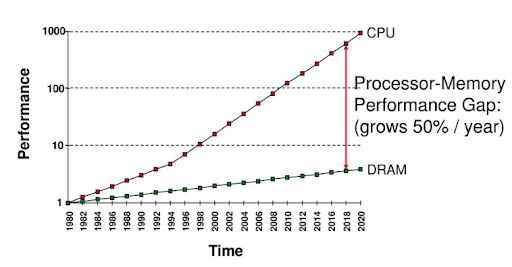
\includegraphics[scale=0.7]{images/gap-processor-memory.png}\\
  \footnotesize{Retirado de: http://mirkwood.cs.edinboro.edu/~bennett/class/csci312/fall2018/notes/five/one.html}
  \label{fig:processor-memory-performance-gap}
\end{figure} 
Apesar das melhorias feitas por cada uma destas indústrias ao longo dos anos, a disparidade de desempenho dos dois componentes fazem com que o processador imponha demandas significativas à memória, que em um cenário real não podem ser supridas, gerando assim um sistema desequilibrado, e então, devido a baixa largura de banda da memória em comparação ao alto desempenho do processador temos um aumento no tempo gasto para concluir uma solicitação, afetando diretamente o desempenho das aplicações. Para suprir esse desequilíbrio os projetistas de computadores criaram o que conhecemos como hierarquia de memória, que consiste em conectar o processador  `a um conjunto hierárquico de memórias, cada uma das quais maior, mais lenta e mais barata (por byte) do que as memórias mais próximas ao processador` \cite[tradução nossa]{paper-gap-between-processor-memory}.

Nas arquiteturas computacionais modernas essa hierarquia é formada por: registradores, cache, memória primária e memória secundária. A \figref{fig:hierarquia-de-memoria}  demonstra uma hierarquia de memória, seus respectivos valores de latência\footnote{Tempo entre o início e conclusão de uma solicitação do processador a memória.}  e espaço para cada nível de um servidor e de um dispositivo móvel hipotético. Através dessa figura é possível observar que, à medida que nos distanciamos do processador, as unidades de tempo variam de centenas de picossegundos até milissegundos, ao passo que a capacidade de armazenamento varia de bytes para terabytes.

Devido  a alta latência que as memórias mais distantes do processador possuem, torna-se ideal trabalhar nos níveis superiores da hierarquia de memória para obter um desempenho efetivo das operações sobre um conjunto de dados  \citep{book-compact-data-structures}. A grande problemática é que, conforme disposto por \cite{paper-gap-between-processor-memory}, as memórias com latência menor possuem capacidade de armazenamento também menor, tornando praticamente inviável manipular grandes conjuntos de dados nestes níveis, o que é cada vez mais necessário nos dias atuais, devido ao aumento crescente na produção e consumo de dados. Uma possível solução para tanto é operar sobre os dados em sua forma compactada, e conforme cita também \cite{coira-feranando}, a melhor maneira de fazer isso é através do uso das estruturas de dados sucintas.
%TODO: melhor pelo paragŕafo abaixo
\begin{figure}[!ht]
\centering
  \caption[Exemplos de representação gráficas de árvores]{Os níveis em uma hierarquia de memória em um servidor (a) e em um dispositivo pessoal móvel (PMD) (b).}
  \subfigure[ref1][Hierarquia de memória de um servidor]{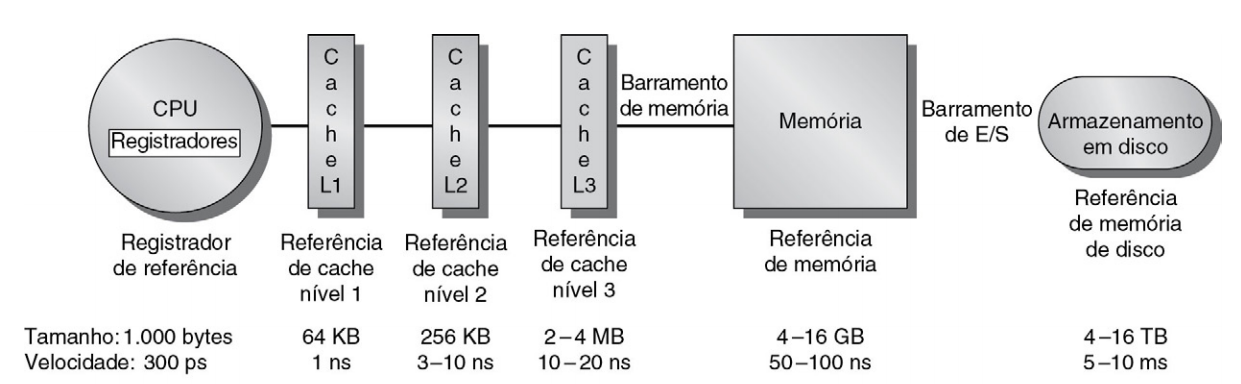
\includegraphics[width=\columnwidth]{images/servidor.png}}
  \qquad
  \subfigure[ref1][Hierarquia de memória de um dispositivo móvel]{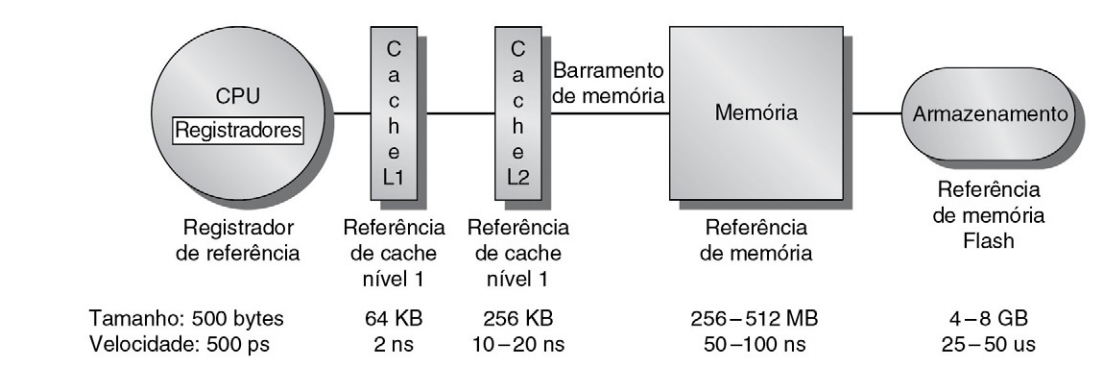
\includegraphics[width=\columnwidth]{images/mobile.png}}
  \footnotesize{Fonte: \citet{book-computer-architecutre}}
  \label{fig:hierarquia-de-memoria}
\end{figure}
Possuindo relação direta com a Teoria da Informação\footnote{Teoria matemática proposta inicialmente por Claude Shannon que busca quantificar a informação.}, uma estrutura de dados é dita sucinta se ela pode representar informações usando um espaço próximo à entropia\footnote{Número mínimo de bits necessários para diferenciar um objeto em um conjunto de dados.} determinada por essa teoria, que como mostra \cite{book-compact-data-structures},  em seu livro, no pior caso é de $\log_2 |U|$ bits para um objeto de cardinalidade $U$. Além disso, essa estrutura deve fornecer suporte a uma série de operações primitivas sobre os seus objetos de modo eficiente. Por fim, uma estrutura de dados sucinta é considerada mais eficiente do que outros algoritmos de compactação clássicos, porque estes precisam descompactar os dados antes de operar sobre os mesmos \citep{coira-feranando}, tornando inviável a manipulação de grandes conjuntos de dados em memórias como a cache e a RAM, ao paso que nas estruturas de dados sucintas, não é necessário descompatar a informação para operar sobre ela.


\section{Árvores Sucintas}
`Sendo uma das estruturas de dados mais difundidas na computação, as árvores também são uma das histórias de sucesso mais marcantes nas estruturas de dados sucintas` \cite[tradução nossa]{book-compact-data-structures}. Uma árvore $T=(V,E)$ é uma estrutura de dados hierárquica, ou seja não linear, formada por vértices (V) e arestas (E). Assim, árvores são definidas também como grafos, sendo eles conexos, não dirigidos e acíclicos, ou seja para qualquer dois vértices em $T$ existe um único e simples caminho \citep{book-algoritmos-teoria-pratica}.

 
Encontramos diversas aplicações construídas a partir destas estruturas, entre elas aplicações de banco de dados e tradutores de idiomas \citep{book-algoritmos-teoria-pratica}. Árvores também são amplamente usadas no campo de aprendizagem de máquina: são as chamadas árvores de decisão, que auxiliam desde a escolha do melhor movimento em um jogo de xadrez  à operações em sites de comércio eletrônico \citep{book-inteligencia-artificial}. Outra aplicação das árvores no mundo real, se dá através do mapeamento de \textit{Domain Name System (DNS)} em endereços \textit{IP} (e virse-versa). Como mostra  \citep{arvore-dns}  a aŕvore de \textit{DNS} representa de modo hierárquico os nomes de um domínio, facilitando a sua administração e escalonamento. O \textit{DNS} é armazenado de forma invertida na árvore, e cada nó possuí um rótulo (de até $63$ caracteres), representando um \textit{host} ou \textit{subdomínio}, a raíz, por padrão, recebe um rótulo nulo, e o nome de qualquer domínio pode ser obtido a partir do percurso de um nó folha até chegar ao nó raíz. É possível ver um exemplo de uma árvore de \textit{DNS},  que armazena o domínio \textit{data.structure.trees.com} na \figref{fig:example-tree}, essa figura também exemplifica parte uma árvore de decisão usada em um jogo da velha.

\begin{figure}[!ht]
\centering
  \caption[Exemplos de representação gráficas de árvores]{Exemplos de representação gráficas de árvores}
  \subfigure[ref1][Árvore de DNS, a subárvore enraízada no nó \textbf{com} define o domínio \textit{data.structure.trees.com}]{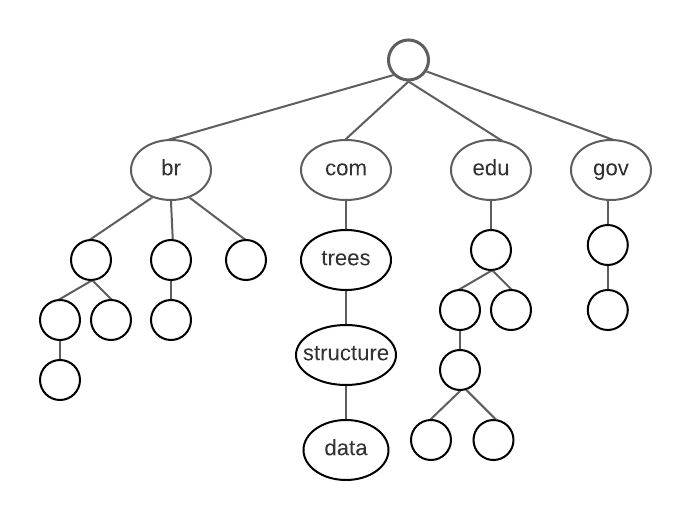
\includegraphics[scale=0.8]{images/tree-dns.png}}
  \qquad
  \subfigure[ref1][Segmento de uma árvore de decisão para um jogo da velha]{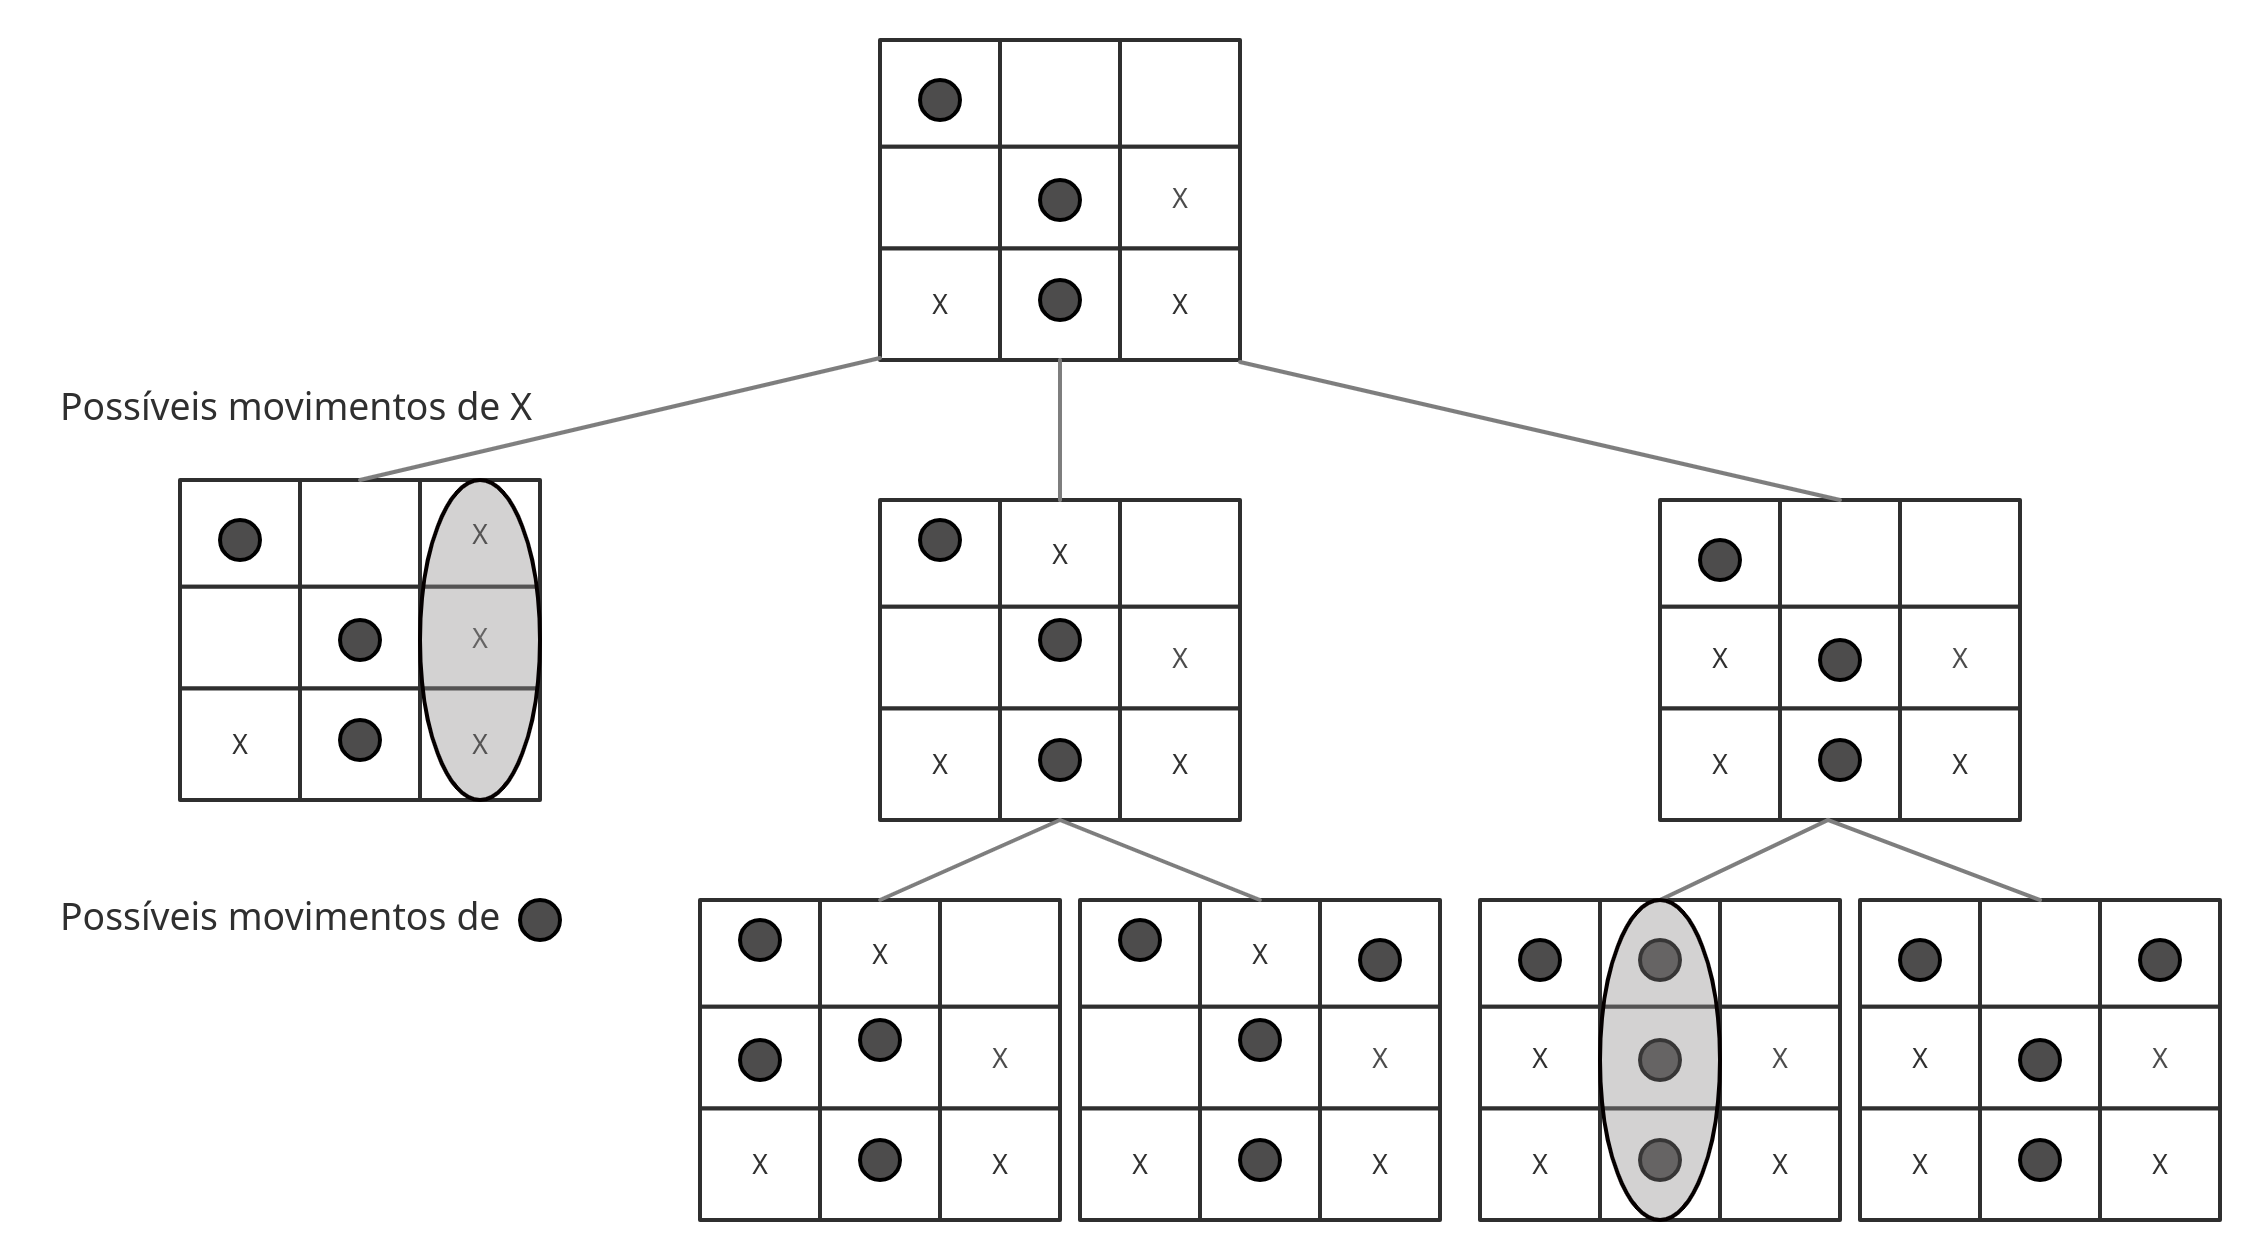
\includegraphics[width=\columnwidth]{images/decision-tree.png}}
  \label{fig:example-tree}
\end{figure}

Mesmo estruturas eficientes como as árvores podem se tornar inviáveis para determinadas aplicações. A forma como estas são construídas afim de operar sobre os objetos podem muitas vezes ocupar um espaço ainda maior do que os dados ocupariam originalmente. Para reconhecer este problema \citet{book-compact-data-structures}, traz como exemplo uma comparação do espaço ocupado pelo genoma humano armazenado sem estruturas adicionais, e o espaço ocupado pelo mesmo usando uma árvore de sufixos que viabiliza operações de montagem de genomas. Com  3,3 bilhões de nucleotídeos, se usarmos 2 bits para armazenar cada base nitrogenada necessitaremos de aproximadamente 825 megabytes, assim podemos reter o DNA por completo em qualquer memória principal, no entanto. Usando a árvore de sufixos, cada nucleotídeo precisará de 10 bytes para ser representado, o que nos leva a uma estrutura que ocupa um espaço igual à 33 gigabytes, o que torna inviável o processamento do genoma em memória principal em computadores comuns. %Fazendo com que seja necessário armazenar parte do mesmo em memórias como o disco, o que como já vimos acarreta em um alto custo computacional.

É nesse ponto que entram as estruturas de dados sucintas. Como já vimos, estas são capazes de armazenar tanto as informações, como as estruturas de dados que atuam sobre elas usando um espaço reduzido. No caso das árvores que é o objeto do nosso estudo, a sua representação clássica com ponteiros  ocupa  $O(n \log n)$ bits\footnote{Neste trabalho, quando não indicado, estaremos trabalhando com o logarítmo na base 2.}, enquanto existem representações sucintas, abordadas nas Seções \ref{sec:sec-bitvector} e \ref{sec:sec-parenthesis-balanceados}, que ocupam cerca de $2n+o(n)$ bits.

\section{Vetores de Bits}\label{sec:sec-bitvector}
Um vetor de bits $BV[0,n-1]$  é uma sequência sobre o alfabeto $\Sigma = \{0,1\}$. É interessante que as seguintes operações sejam executadas sobre os vetores de bits \citep{book-compact-data-structures}:

\begin{itemize}
    \item $access(BV,i)$: retorna o $i-$ésimo bit do vetor $BV$, com $0 \leq i < n$;
    \item $rank_v(BV,i)$: seja $v \in \{0,1\}$, e $0 \leq i < n$, esta operação retorna o número de ocorrências de $v$ no intervalo $BV[0,i]$.\\
    Sendo que a seguinte relação de equivalência é válida: $rank_0(BV,i)=i +1  - rank_1(BV,i)$;
    \item $select_v(BV,i)$: dado $v \in \{0,1\}$, com $0 \leq i < n_v$, e sendo $n_v$ o número máximo de ocorrências de $v$ em $BV$,
    $select$ retorna a posição do $i-$ésimo bit $v$ em $BV[0,n-1]$.
\end{itemize}

A \figref{fig:bitvector-operations} traz exemplos das operações listadas.
\begin{figure}[!ht]
\centering
  \caption[Operações sobre vetores de bits]{Operações de $rank, select$ e $access$ sobre $B=111010011000$}
  \subfigure[Operação de $access$ sobre $B=111010011000$][$access(BV,4)=1$]{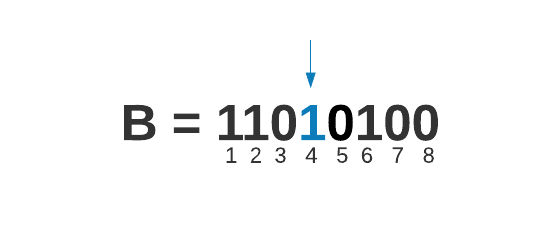
\includegraphics[scale=1.0]{images/access.png}}
  \subfigure[Operação de $rank$ sobre $B=111010011000$][$rank_1(BV,6)=4$]{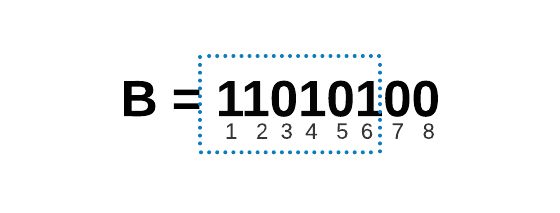
\includegraphics[scale=1.0]{images/rank.png}}
  \subfigure[Operação de $select$ sobre $B=111010011000$][$select_0(BV,5)=8$]{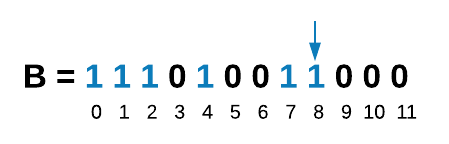
\includegraphics[scale=1.0]{images/select.png}}
  \label{fig:bitvector-operations}
\end{figure}

\section{Representação de árvores sucintas}
Existem diversas formas de representar  uma árvore de maneira sucinta, abaixo listamos algumas destas.

\subsection{Parênteses Balanceado (BP)}\label{sec:sec-parenthesis-balanceados}
\begin{figure}[!ht]
\centering
  \caption[Representação de árvores com parênteses balanceados]{Representação de uma árvore $T$ usando parênteses balanceados: fazendo um percurso pré-ordem em $T$ escrevemos um parênteses de abertura quando um nó é visitado pela primeira vez, e um de fechamento no percurso de volta após atravessar  sua subárvore \citep{paper-succint-representation-of-balanced-parentheses}}
  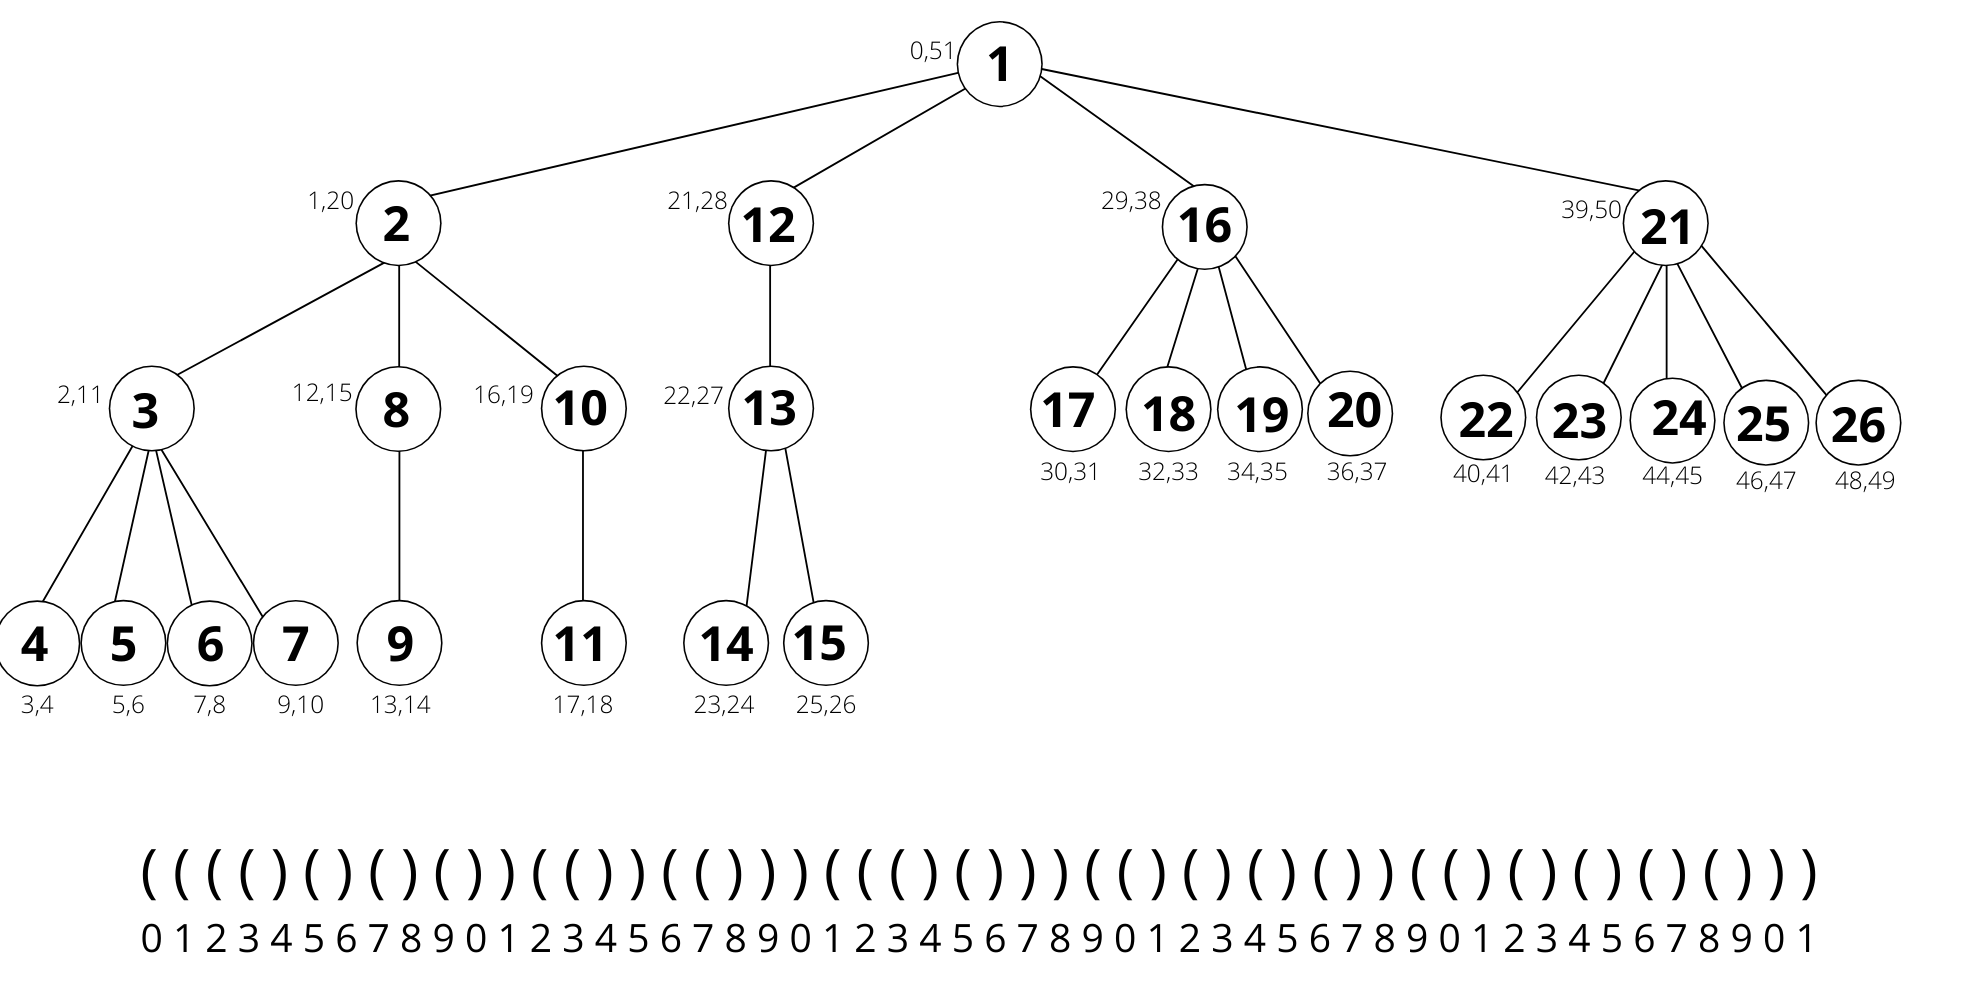
\includegraphics[width=\columnwidth]{images/arvore_geral.png}
  \label{fig:parenthesis-representation}
\end{figure}
Uma sequência de parênteses balanceados (BP) consiste em uma string de tamanho igual à $2n$, sendo $n$ parênteses de abertura '(', e $n$ parênteses de fechamento ')'. Essa estrutura descreve uma relação de hierarquia/contenção, e portanto é amplamente utilizada para a representação de árvores.

Para representar uma árvore ordinal\footnote{Em uma árvore ordinal, cada nó pode ter um número árbitrário de filhos, e as subárvores de cada nó formam um conjunto ordenado de nós \citep{tenenbaum}} $T$ usando essa estrutura, tomamos um vetor de bits de tamanho igual à $2n$ ($BP[0,2n-1])$, em que $n$ é o número de nós da árvore. Realizamos então um percurso sobre $T$ em pré-ordem, e sempre que um nó for alcançado pela primeira vez, um parênteses de abertura (podendo ser representado pelo bit $1$) é inserido em $BP$, ao término da exploração das subárvores deste nó, um parênteses de fechamento (bit $0$) é adicionado em $BP$ \citep{paper-succint-trees-in-practice}.  Na figura \figref{fig:parenthesis-representation} pode-se observar uma árvore com 26 nós e sua representação equivalente em parênteses balanceados.
%Para representar uma árvore ordinal $T$ usando essa estrutura tomamos um vetor de tamanho igual à $2n$ ($BP[0,2n-1])$ onde $n$ é o número de nós da árvore. O nó $v$ (codificado em $BP[i]$) da árvore $T$ é representado por um parênteses de abertura e um de fechamento em $BP$, os elementos contidos no intervalo aberto desses parênteses codificam as subárvores de $v$ em ordem de igual maneira. Na figura \figref{fig:parenthesis-representation} vemos um árvore com 14 nós e sua representação equivalente em parênteses balanceados.

Usando a representação de parênteses balanceados, podemos fornecer suporte às operações descritas a seguir para diversas estruturas de dados sucintas:
\begin{itemize}
    \item $findclose(BP,i)$: retorna a posição $j$ do parênteses de fechamento, correspondente ao i-ésimo parênteses de abertura;
    \item $findopen(BP, i)$: retorna a posição $j$ do parênteses de abertura, correspondente ao i-ésimo parênteses de fechamento;
    \item $excess(BP, i)$: retorna a `diferença entre o número de parênteses abertos e fechados até a posição $i$`.  \cite[tradução nossa]{paper-succint-representation-of-balanced-parentheses}
\end{itemize}

\citet{paper-succint-representation-of-balanced-parentheses} proporam uma solução em árvores binárias usando a representação de parênteses balanceados, nesta proposta,  além das operações já citadas, os autores viabilizaram suporte a operação de $enclose(i)$, que retorna o pai de um nó codificado em $i$,  e a operação $double\_enclose(i,j)$ (que equivale à operação $lca$ em árvores) que por sua vez retorna o ancestral comum mais baixo dos nós $i$ e $j$. 

Com base na operação  $rank$ podemos viabilizar a operação de $excess$ facilmente, como mostrado abaixo.

\begin{eqnarray*}
    \begin{split}
        excess(BP,i) &= rank_1(BP,i) - rank_0(BP,i) \\
        &  = rank_1(BP,i) - (i - rank_1(BP,i)) \\
        &  = 2 \cdot rank_1(BP,i) - i -1 
    \end{split}
\end{eqnarray*}

Através das operações definidas em vetores de bits e parênteses balanceados, podemos fornecer suporte às diversas operações sobre árvores, como a obtenção do tamanho da subárvore de um nó $i$, que pode ser feita através de: $(findclose(BP,i)+i-1)/2$. Esta expressão retornará a quantidade de nós codificados dentro do intervalo de contenção de $i$. 

Levando em consideração que em $BP$ um nó é codificado através de um parênteses de abertura, podemos responder facilmente se um nó codificado $j$ é ou não, um nó folha, para tanto, basta averiguar se o elemento que segue o índice $j$, codifica um novo nó, em caso afirmativo, o nó codificado por $j$ possuí filhos, e portanto não pode ser um nó folha, caso o elemento armazezando em $j+1$ corresponda à um parênteses de fechamento significa que o nó $j$ não possuí filhos, e portanto é um nó folha. Esta verificação pode ser feita através da operação de $access(BP,j+1)$.

Por fim, uma das vantagens da \textit{sequência de parênteses balanceados}, como cita \cite{book-compact-data-structures}, é que a mesma permite que qualquer subárvore de um nó, seja mapeada de forma contígua em um vetor de bits, o que simplifica uma série de operações existentes sobre árvores.

\subsection{Depth-First Unary Degree Sequence (DFUDS)}
Outra forma de representar árvores é atráves da \textit{Depth-First Unary Degree Sequence}, que assim como em $BP$ faz o uso de uma travessia pré-ordem para construir a árvore à qual representa.
A diferença é que  para codificar um nó, inserimos $i$ parênteses de abertura (onde $i$ é o número de filhos deste nó) e $1$ parênteses de fechamento.  Desse modo, conforme afirma \cite{paper-succint-trees-in-practice}, o nó passa a ser representado pela posição de seus $i$ parênteses de abertura. A \figref{fig:dfuds-representation}, mostra a representação equivalente à de parênteses balanceados, usando \textit{DFUDS}.
\begin{figure}[!ht]
    \centering
      \caption[Representação de árvores com Sequência de Grau Unário]{Representação de uma árvore $T$ usando DFUDS. O primeiro parênteses (em negrito) não codifica nenhum nó, e foi adicionado ao início da sequência  para que a mesma se tornasse balanceada.}
      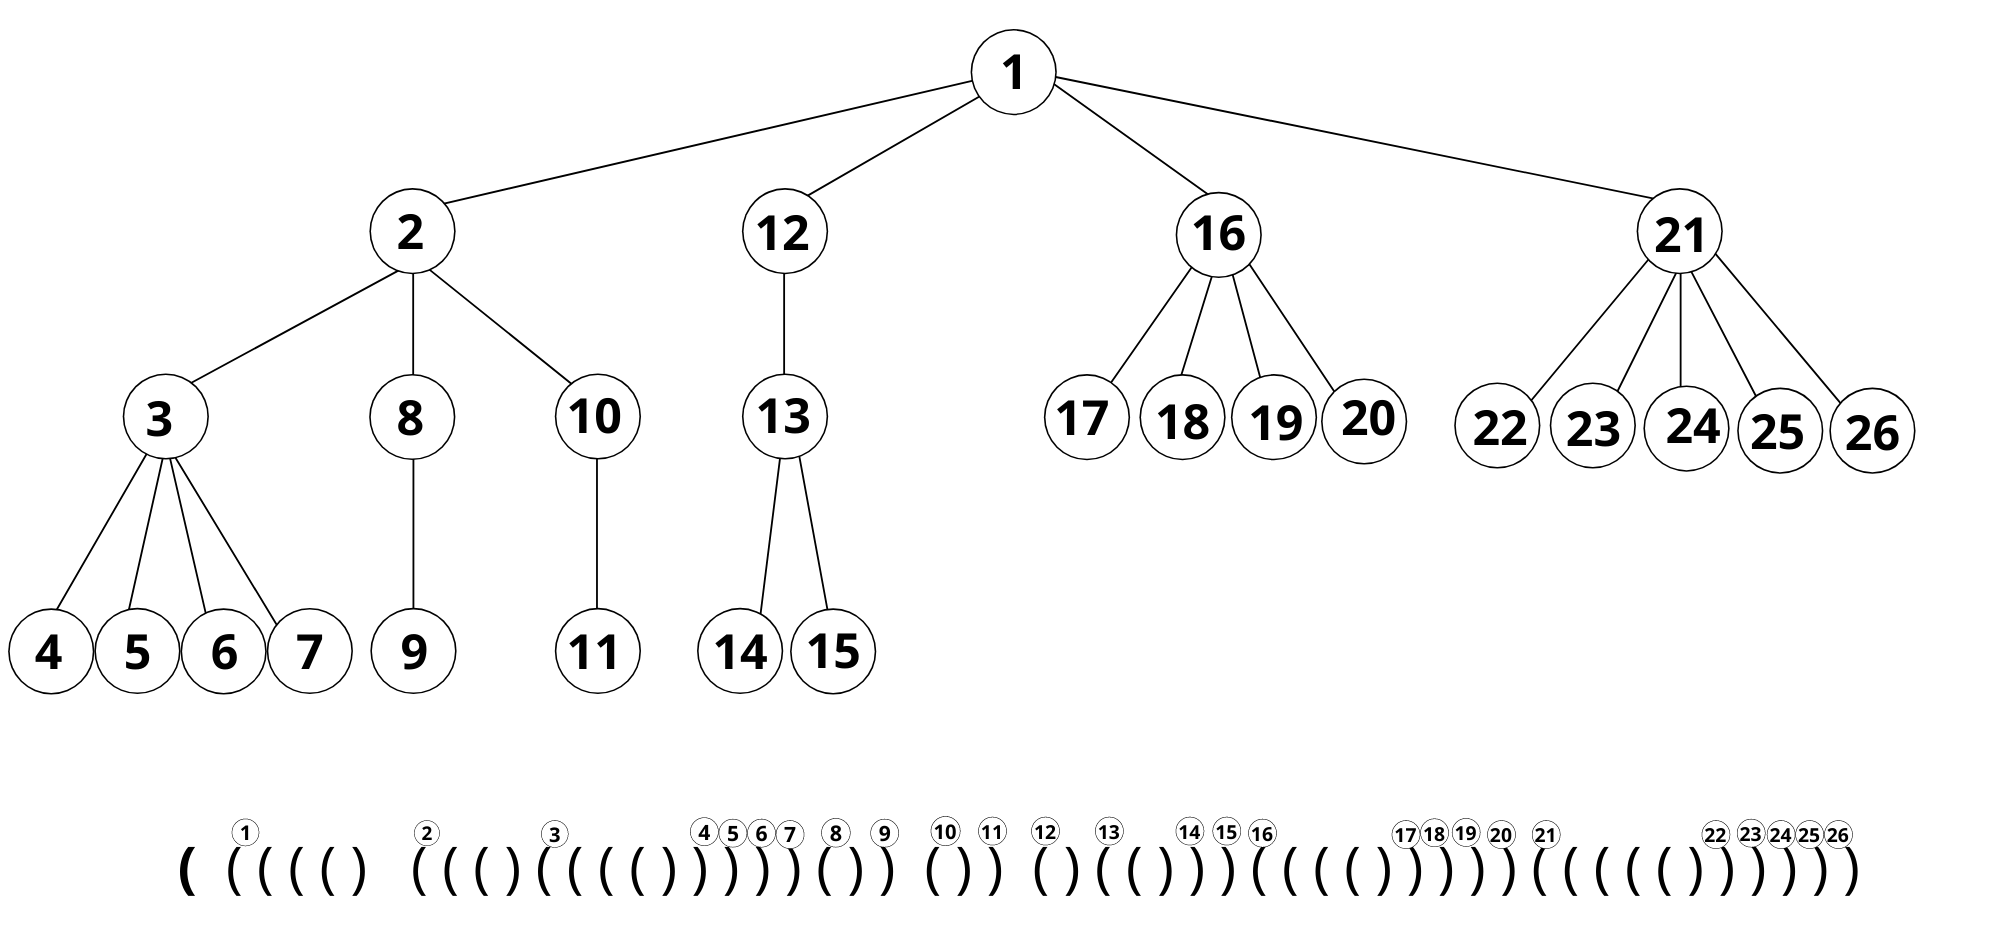
\includegraphics[width=\columnwidth]{images/dfuds.png}
      \label{fig:dfuds-representation}
\end{figure}

Como um nó nessa representação é codificado através do parênteses de abertura (ou bit $1$) de seus $i$ filhos, adicionado de um parênteses fechamento, temos que a sequêrncia gerada em \textit{DFUDS} não é totalmente balanceada, apresentando $n-1$ parênteses de abertura (como sabemos um nó raíz não possuí pai, e portanto, seu parênteses de abertura não é codificado na sequência), e $n$ parênteses de fechamento.  Afim de deixar a sequência balanceada, podemos adicionar um parênteses de abertura ao início da mesma, como é feito em \citet{paper-succint-trees-in-practice}.

\citet{book-compact-data-structures} afirma em seu trabalho, que nessa representação é mais  rápido descer até o $i-$ésimo filho de um nó de uma árvore $T$. Bastando avançar  $i$ posições a partir do ínicio da codificação de um nó, no vetor que contém a sequência. Ademais, assim como em $BP$, qualquer subárvore de um nó, é mapeada de modo contíguo em um vetor, entretanto, a área dessa subárvore não pode ser delimitada por um parênteses de fechamento, como acontece para \textit{parênteses balanceados} \citep{book-compact-data-structures}.

\subsection{Level-order Unary Degree Sequence (LOUDS)}
Nesta representação, pecorremos os nós da árvore em largura, adicionando assim como em \textit{DFUDS}, $i$ (novamente com $i$ representando o grau do nó) parênteses de abertura ao visitarmos um nó pela primeira vez, seguido de $1$ parênteses de fechamento.
 Como os nós são codificados através de um percurso em largura na árvore de entrada, essa estrutura não permite que as subárvores de um nó sejam mapeadas de forma contígua no vetor que a representa, inviabilizando operações básicas como o cálculo do tamanho da subárvore de um nó \citep{book-compact-data-structures,paper-fully-functinal-succint-trees}.

A figura abaixo mostra uma representação em \textit{LOUDS} para a árvore $T$, usada como exemplo na representação de \textit{parênteses balanceados} e em \textit{DFUDS}.

\begin{figure}[!ht]
    \centering
      \caption[Representação de árvores com Level-order Unary Degree Sequence]{Representação de uma árvore $T$ usando LOUDS. 
      Assim como em DFUDS foi adicionado um parênteses de abertura no início da sequência  para que a mesma se tornasse balanceada.}
      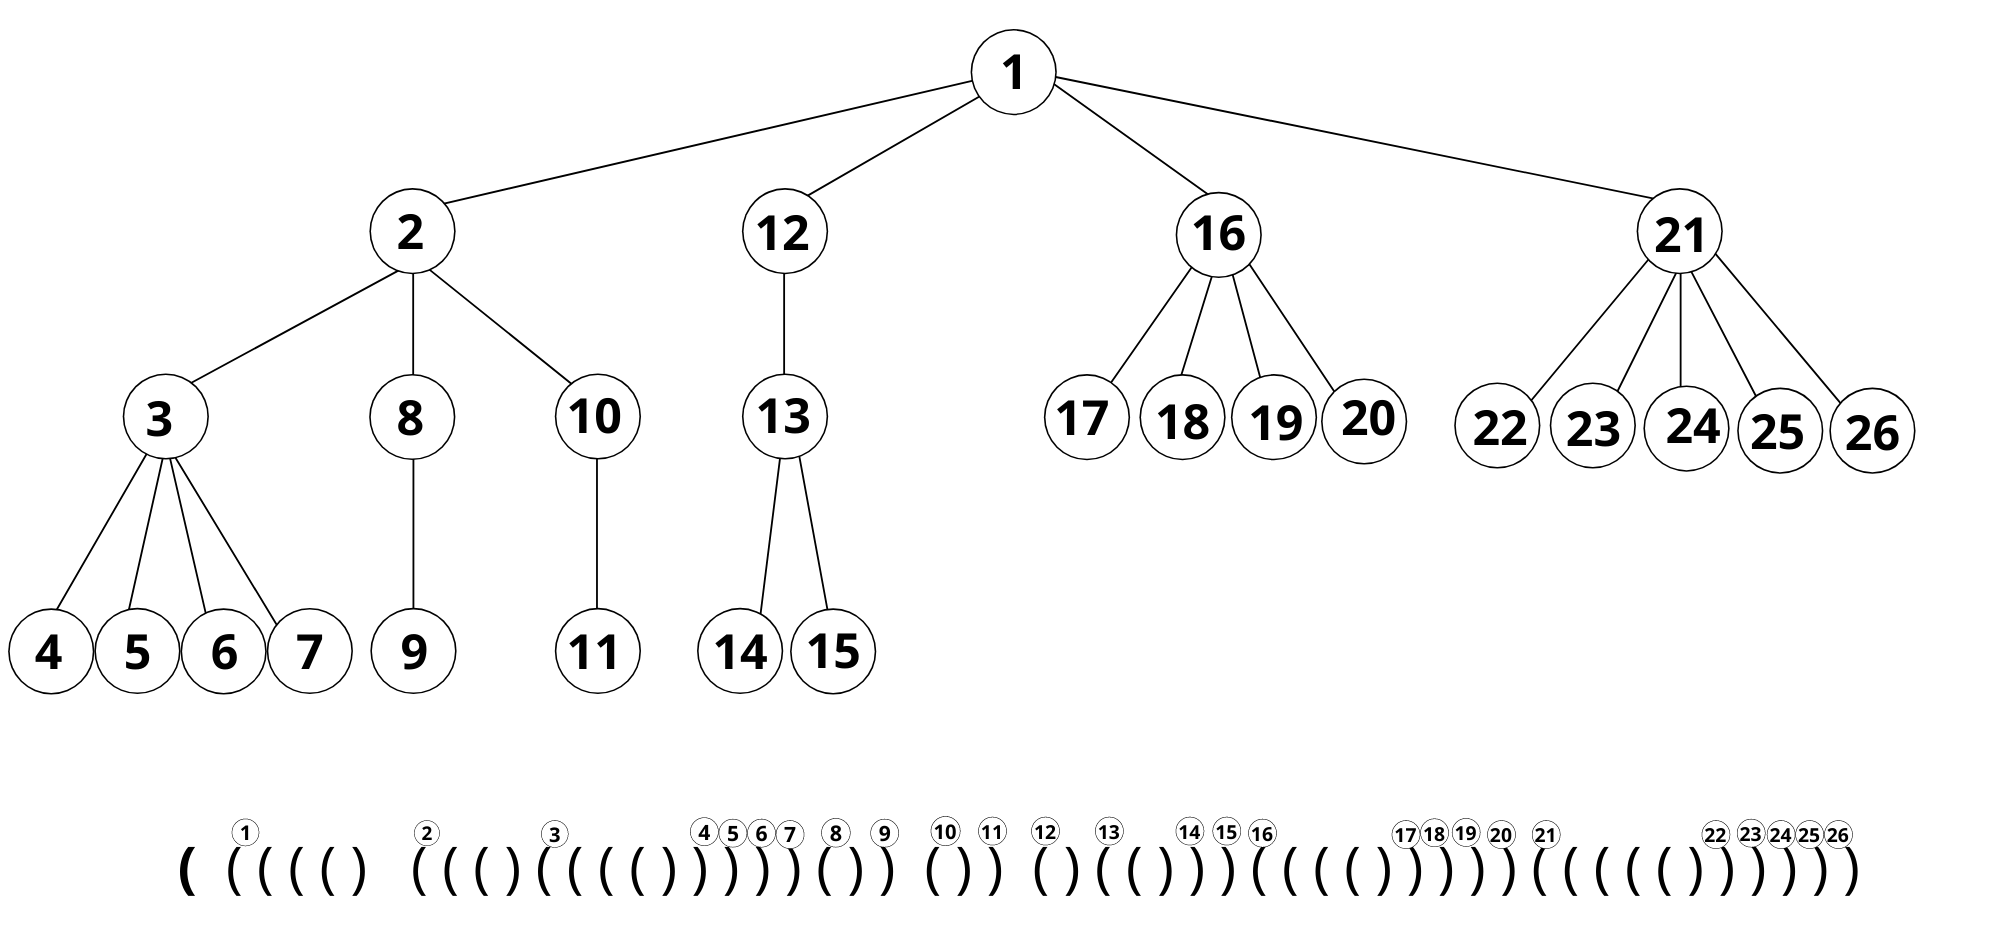
\includegraphics[width=\columnwidth]{images/dfuds.png}
      \label{fig:dfudus-representation}
\end{figure}

\section{Range min-Max Tree (rmM-tree)}\label{sec:sec-classic-rmm-tree}
Proposta por \citet{paper-fully-functinal-succint-trees}, estudada por diversos outros autores, a range min-Max tree, é uma estrutura baseada em valores de excessos máximos e mínimos dentro de um intervalo. Esta é contruída com base em uma sequência de parênteses balanceados, e permite a redução de um grande número de operações relevantes sobre árvores consideradas na literatura, a poucas operações primitivas, podendo estas serem realizadas em tempo constante para árvores suficientemente pequenas \citep{paper-fully-functinal-succint-trees}.

Neste trabalho usaremos a abordagem mostrada por \citet{book-compact-data-structures} em seu livro, para a construção da rmM-tree binária. Como explica o autor, a range min-Max tree é construída na forma de uma árvore binária completa --o que nos permite a utilização de vetores, omitindo o uso de ponteiros explícitos -- sendo que cada um de seus nós armazena os valores de excesso calculados dentro de um intervalo do vetor que representa a árvore de entrada. 

A construção da rmM-tree segue uma abordagem \textit{bottom-up}, onde a cada nó, calcula-se primeiro o intervalo a ser coberto, para então definirmos os  valores de excesso. Após construir os nós folhas dessa estrutura, repetimos o processo descrito para os nós internos (e raíz), sendo que o intervalo coberto por cada nó não folha é dado pela união da área coberta pelos seus nós filhos.

%A quantidade de intervalos armazenados por essa estrutura influência diretamente na complexidade de espaço ocupado pela mesma. 
Como cada nó folha de uma rmM-tree está associado a um único intervalo, o tamanho de uma rmM-tree está também relacionado a quantidade e ao tamanho dos intervalos cobertos pela mesma. 
Esses intervalos são obtidos da seguinte maneira: dado um vetor de entrada $BP$, de  tamanho igual à $n$, sendo $BP$ usado para a codificação via parênteses balanceados de uma árvore $T$ com tamanho igual à $n/2$, é definido um tamanho de intervalo $b$ (chamado também de tamanho de bloco), divide-se então $n$ por $b$, obtendo assim a a quantidade de folhas da rmM-tree.

Considerando que a altura de uma árvore binária é dada por $\lceil \log n \rceil$ e que o vetor de entrada $BP$ ocupa $n$ bits, temos assim que a rmM-tree utiliza um espaço próximo à $n + O(\frac{n}{b} \log n)$ bits. Tomando $b = \log^2 n$, temos uma complexidade de espaço igual à $n + O(n/\log n)$. Em relação ao tempo gasto por cada operação sobre a rmM-tree,  \citet{book-compact-data-structures} mostra que na prática todas essas operações podem ser realizadas em tempo $O(\log n)$ - ou ainda em tempo $O(\log \log n)$ em uma versão mais refinida da estrutura - a lista completa dessas operações é apresentada na \tabref{tbl:classicOperations-rmm-tree} deste capítulo.
%TODO: b é fixado em log^2n, o que nos dá $n + O(\frac{n}{\log n}$ bits$

\subsection{Registros}
Os valores de excesso definidos em cada nó da rmM-tree são essenciais para a realização de operações de consulta de maneira eficiente, são neles em que essa estrutura se baseia.  Em seu livro, \citet{book-compact-data-structures}, define 4 valores de excesso que viabilizam essas operações. Mostraremos as definições de cada um destes a seguir. 

Suponha que um nó $v$ cubra um intervalo $[s,e]$ do vetor de entrada $BP$ definido anteriormente, então:
\begin{itemize}
    \item \textit{R[v].e}: armazena o excesso total no intervalo $[s,e]$.
    
    $R[v].e = excess(e) - excess(s-1)$.
    \item \textit{R[v].m}: corresponde ao excesso mínimo local.
    
    $R[v].m = \min\{excess(i) - excess(s - 1) | s \leq i \leq e\}$.
    \item \textit{R[v].M}: corresponde ao excesso máximo local.
    
    $R[v].M = \max\{excess(i) - excess(s - 1) | s \leq i \leq e\}$.
    
    \item \textit{R[v].n}: é definido pelo número de vezes que o excesso mínimo ocorre dentro do intervalo coberto. Assim, suponha $m$ o valor do excesso mínimo no intervalo $[s,e]$, então:

    $R[v].n = |\{s \leq i \leq e | excess(i) = R[v].m\}|$
    %$R[v].n= |{p \in BP[s,e], excess(p) - excess(s - 1) = R[v].m}|$
\end{itemize}

    Agora que temos a definição de cada registro da range min-Max tree, podemos construir os nós folhas da nossa estrutura, e os demais nós nível a nível, partindo das folhas. Os nós internos e raíz da nossa árvore, são calculados a partir dos valores de seus nós filhos, como a nossa estrutura é construída em um vetor, podemos navegar até os filhos de um nó $v$ usando aritmética básica nos índices da nossa árvore, desse modo, o filho esquerdo de um nó $v$ é dado por $(2 \cdot v)+1$, ao passo que o filho direito desse nó pode ser obtido a partir de $(2 \cdot v) +2$. Essa relação entre os valores dos registros de um nó pai e um nó filho, é descrita pelas equações abaixo:

    \begin{itemize}
        \item $R[v].e = R[2v +1 ].e + R[2v + 2].e$
        \item $R[v].m = min(R[2v+1].m, R[2v+1].e + R[2v + 2].m)$
        \item $R[v].M = max(R[2v+1].M, R[2v+1].e + R[2v + 2].M)$
        \item $ R[v].n =
           \begin{cases}
                 R[2v+1].n, & \mbox{se } R[2v+1].m < R[2v+1].e + R[2v + 2].m; \\
                 R[2v + 2].n, & \mbox{se } R[2v+1].m > R[2v+1].e + R[2v + 2].m; \\
                 R[2v+1].n + R[2v + 2].n, & \mbox{se }  R[2v+1].m = R[2v+1].e + R[2v + 2].m .
           \end{cases}
        $
    \end{itemize}

\begin{example}\label{ex-build-tree}
    Para melhor elucidar a construção dessa estrutura usaremos o exemplo da Seção~\ref{sec:sec-parenthesis-balanceados} e demonstraremos o cálculo dos registros e dos intervalo de um nó folha, mostraremos também como é construído um dos nós internos da rmM-tree. No exemplo em questão, temos um vetor de entrada com 52 parênteses balanceados, e um tamanho de bloco $b = 4$ o que implica que a árvore terá:

    \begin{itemize}
        \item $r = n/b \to r = 52/4 = 13 $ folhas;
        \item 12 nós internos, pois $r-1 = 12$;
        \item Altura $h= \ceil{\log r} \to h = \ceil{\log 13}= 4$;
        \item Como o número de folhas não é uma potência de 2, temos que as folhas $0$ até $2 \cdot r - 2^h  -1 = 9$ estão agrupadas no último nível da árvore,  e as outras $2^h - r = $ folhas estão agrupadas à direita no nível anterior.
    \end{itemize}

    Assim temos os seguintes valores de excesso para a folha $0$ (nó $15$) da rmM-tree:
        \begin{itemize}
            \item  Área de cobertura:
            $ BP[0,3]$
            \item Excesso local:
            $R[15].e = excess(3) = 2 \cdot rank_1(BP,3) - 3 - 1= 4$
            \item Excesso mínimo:
            $R[15].m = min(1,2,3,4) = 1$
            \item Excesso máximo:
            $R[15].M = max(1,2,3,4) = 4$
            \item Número de vezes que o excesso mínimo ocorre no intervalo:\\
            $R[15].n = count(1,2,3,4) = 1$
        \end{itemize}
        
    Mostraremos agora o cálculo do 7º nó interno do nosso exemplo, este cobre as folhas 0 e 1 da árvore (nós 15 e 16, respectivamente), com base nas definições anteriores temos então:
    \begin{itemize}
        \item Área de cobertura: $BP[0,3] \cup BP[4,7]$
        \item Excesso global: \\
        $R[7] = R[15].e + R[16].e = 4 + 0 = 4$
        \item Excesso mínimo:\\
        $R[7].m = min(R[15].m, R[15].e+R[16].m) = (1,4-1)=1$
        \item Excesso máximo:\\
        $R[7].M = max(R[15].M, R[15].e+R[16].M) = (4,4+0)=4$
        \item Número de vezes que o excesso mínimo ocorre no intervalo:\\
        $R[7].n = R[15].n = 1$,  pois $R[15].m < R[15].e+R[16].m$
    \end{itemize}

    O processo mostrado acima deve ser repetido para os demais nós da árvore até que cheguemos a raíz, dando origem a árvore mostrada na \figref{fig:rmm-tree-binaria}. 
    \begin{figure}[!ht]
     \centering
      \caption[rmM-tree clássica.]{rmM-tree clássica,com tamanho de bloco igual à 4. A estrutura foi construída a partir dos 52 parênteses balanceados mostrados na parte inferior}
      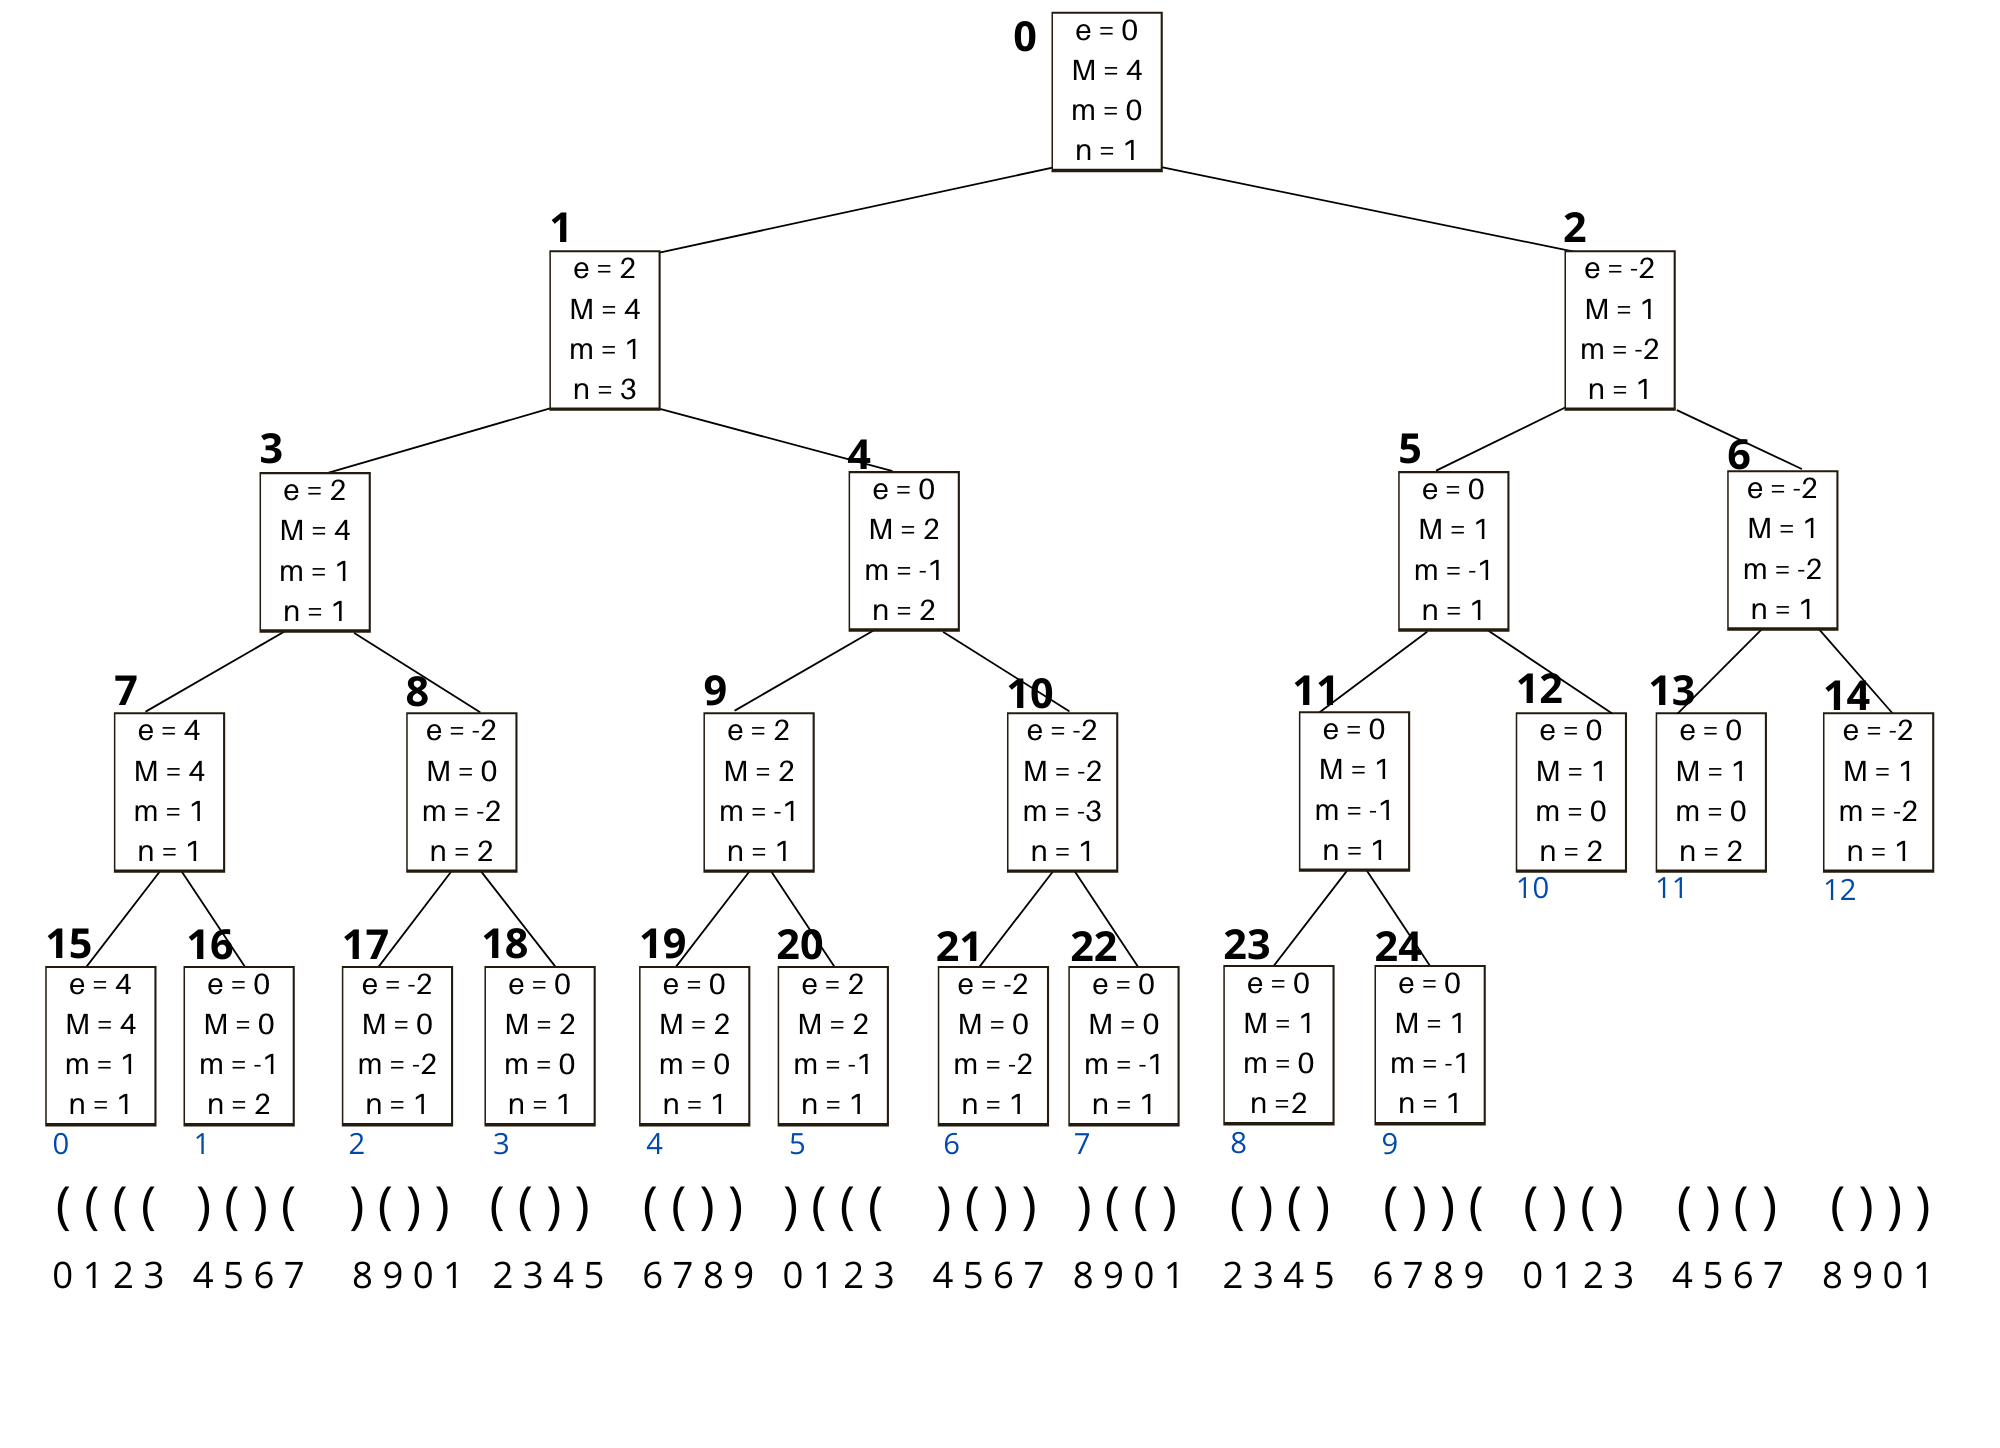
\includegraphics[width=\columnwidth]{images/rmm-tree-bin.png}
      \label{fig:rmm-tree-binaria}
    \end{figure}
\end{example}

O processo de construção da rmM-tree é mostrado com mais detalhes no Algoritmo~\ref{alg:build-bin-tree}. Neste algoritmo, fazemos o uso de uma tabela $C$, esta tabela pré-computa todas as possibilidades de valores de registro para um intervalo tamanho $w$, sendo $b \mbox{ mod } w = 0$. `Essa técnica de pré-computar todos os valores possíveis de determinados padrões de bits é conhecida como \textit{truque dos quatro russos}` \citep[tradução nossa]{book-gusfield}.
O uso dessa tabela $C$ não é obrigatório para a construção da rmM-tree, entretanto, a mesma possibilita a otimização do tempo de construção e operação sobre a rmM-tree, como disposto em \citet{book-compact-data-structures}.

Conforme expõe \citet{book-compact-data-structures}, a tabela $C$ é construída em tempo $O(\sqrt{n} \log n)$ e ocupa $O(\sqrt{n} w)$ bits de espaço. Esse processo de construção é feito do seguinte modo: após definir uma constante $w$, criamos uma tabela $C[0, 2^w-1]$,  onde cada entrada da tabela armazena os registros de excesso definidos anteriormente, cada elemento $C[x]$ é calculado com base nos $w$ bits  que formam $x$. Abaixo segue um exemplo explicando a computação de uma entrada específica da tabela $C$.
\begin{example}
    Suponha $w=4$ e $x=3$, temos assim que:

    $$3_2 = 0011,$$  logo iterando sobre os bits que formam o número temos os seguintes valores de  registro:
    \begin{itemize}
        \item $C[x].e = 0; C[x].M = 0; C[x].m = -2; C[x].n = 1$
    \end{itemize}
\end{example}

Fazer a pré-computação dessa tabela elimina a necessidade computar iterativamente os valores de excesso mínimo e máximo, a cada inspeção de bits. Assim, no momento da construção dos nós da rmM-tree, ou durante a inspeção dos mesmos, basta ler os $w$ bits que queremos inspecionar, e então realizar uma consulta na tabela $C$ pelo elemento $x$ que mapeia os bits lidos. Conforme mostra \citet{book-compact-data-structures} uma consulta na tabela $C$ leva tempo constante, já a construção dos nós folhas usando essa técnica leva tempo $O(\frac{n}{\log n})$. A função \textit{bitsread}, atua junto à tabela $C$ otimizando o tempo de resposta das nossas operações, e por esse motivo é usada durante todo o nosso projeto, ela recebe como parâmetro um índice $i$, e então lê a palavra formada a partir de $i$ seguido pelos $w-1$ bits após $i$, usando como critério de leitura o bit mais significativo (\textit{Most Significant Bit (MSB)}). O valor obtido por \textit{bitsread} é usado para consultar a tabela $C$, em busca dos valores de registro correspondentes aos bits analisados. 

Além da tabela $C$ e da função \textit{bitsRead}, em nossa implementação usamos outras duas funções que nos auxiliam no  percurso em árvore, denominadas \textit{leafInTree} e \textit{numLeaf}, a primeira retorna o índice de um nó na rmM-tree correspondente ao número de uma folha,  a segunda por sua vez retorna o número de uma folha correspondente à um nó da rmM-tree (veja Algoritmo~\ref{alg:folha-indice}).

\begin{example}
    Tome como base agora, a nossa rmM-tree de exemplo, assuma $w=4$. Para melhor exemplificação, vamos alterar um pouco a estrutura da nossa árvore, assuma um tamanho de bloco  $b=8$ para este exemplo. Suponha que queremos construir a folha de número $0$ (como aumentamos a cobertura do nosso bloco, a folha $0$ neste exemplo corresponde à união dos nós $15$ e $16$ da árvore mostrada na \figref{fig:rmm-tree-binaria}), que neste exemplo corresponde ao nó $7$. O intervalo coberto por essa folha vai de $0$ à $7$, assim precisaríamos ler os $8$ bits que compõem esse intervalo. 
    
    Para um exemplo pequeno como  este não há problemas em calcular esses valores iterativamente, mas imagine o que acontece com casos em que temos uma árvore de entrada maior, e tamanho de  bloco também maior, o processo se tornaria mais oneroso. Observe então como este processo é feito usando a tabela de excessos $C$.


    \begin{itemize}
        \item Como $w=4$, convertemos primeiro os bits codificados em $BP[0,3]$\\
        $BP[0,1,2,3] = 1111_2$\\
        Fazemos então uma consulta na tabela $C$, pelo elemento $x = 1111_2$, que com base na explicação anterior, traz os seguintes valores:
        $$C[1111_2].e = 4; C[1111_2].M = 4; C[1111_2].m = 1; C[1111_2].n=1.$$
        Nesse momento, os valores do registro da nossa folha são:\\
        $$R[7].e = 4; R[7].M = 4; R[7].m = 1; R[7].n=1.$$
        \item  Agora precisamos computar os valores correspondentes aos $w$ bits restantes que compõem a nossa folha, temos que:
        $BP[4,5,6,7] = 0101_2$. Os registros armazenados em $C$, para este elemento são:
        $$C[0101_2].e = 0; C[0101_2].M = 0; C[0101_2].m = -1; C[0101_2].n=2.$$

        Agora que temos os valores de excesso para cada subintervalo da nossa folha, podemos obter os valores de registro para o intervalo completo, esse processo é similar ao definido para a obtenção dos registros de um nó pai. Temos assim que:
        \begin{itemize}
            \item $R[7].e = R[7].e + C[0101_2].e = 4 + 0 = 4$
            \item $R[7].M = max(R[7].M, R[7].e + C[0101_2].M) =  max(4,4+0) =4$
            \item $R[7].m = min(R[7].m, R[7].e + C[0101_2].m) = min(1,4-1) = 1$
            \item $R[7].n=1,$ pois o excesso mínimo ocorre no primeiro subintervalo da folha.
        \end{itemize}
    \end{itemize}

    Ao observar o nó $7$ do exemplo~\ref{ex-build-tree}, é possível notar, que de fato, os valores obtidos nestes exemplo correspondem ao nó citado.
\end{example}

\begin{algorithm}[htp]
    \SetAlgoLined\DontPrintSemicolon
    \SetKwFunction{algo}{algo}\SetKwFunction{proc}{proc}
    \SetKwProg{myproc}{Proc}{}{}
    \myproc{numLeaf(v)}{
        \Input{Índice $(v)$ da rmM-tree.}
        \Output{Número $(l)$ da folha codificada em $R[v]$.}
        \If{$v \geq 2^h-1$}{\Return{$v - 2^h + 1 $}}
        \Else{\Return{$v - 2^h + r + 1$}}
    }

    \setcounter{AlgoLine}{0}

    \SetKwProg{myproc}{Proc}{}{ }
    \myproc{leafInTree(l)}{
        \Input{Número $(l)$ de uma folha na rmM-tree.}
        \Output{Índice $(v)$ onde a folha é codificada na rmM-tree.}
        \If{$l < (2r - 2^h)$}{\Return{$2^h - 1 + l$}}
        \Else{\Return{$2^h - 1 - r + l$}}
    }
    \caption{Conversão entre número de folha e índice de folha na rmM-tree.}
    \label{alg:folha-indice}
\end{algorithm}

\begin{algorithm}[htp]
    \SetKwFunction{algo}{algo}
    \SetKwProg{myalg}{Algoritmo}{}{}
    \myalg{buildingTree(BP, C, b, w, r, nNodes)}{
        \Input{Vetor de bits, tabela de excessos C, tamanho de bloco e de subbloco, número de folhas e quantidade de nós. }

        \tcp{Construção dos nós folhas}
        \For{$l \leftarrow 0$ \textbf{to} $r-1$}{
            $v \leftarrow leafInTree(l)$\tcp{Algoritmo~\ref{alg:folha-indice}}
            $(R[v].e, R[v].M, R[v].m, R[v].n) \gets(0,-w,w,0)$\\
            \For{$p \leftarrow (l \cdot (b/w))+1$ \textbf{to} $((l+1) \cdot b)/w$}{
                $x \leftarrow bistread((p-1)\cdot w)$\\
                \If{$R[v].e + C[x].M > R[v].M$}{$R[v].M \leftarrow R[v].e + C[x].M$}
                \If{$R[v].e + C[x].m < R[v].m$}{
                    $R[v].m \leftarrow R[v].e + C[x].m$\\
                    $R[v].n \leftarrow 1$
                }
                \ElseIf{$R[v].e + C[x].m = R[v].m$}{$R[v].n \leftarrow R[v].n + C[x].n$}
                $R[v].e \leftarrow R[v].e + C[x].e$
            }
        }

        \tcp{Construção dos nós internos e raíz}
        \For{$v \leftarrow nNodes - r -1 $ \textbf{to} $0$}{
            $v_l \leftarrow (2 \cdot v)+1$\\
            $v_r \leftarrow v_l + 1$\\
            $R[v].e \leftarrow R[v_l].e + R[v_r].e$\\
            $R[v].M \leftarrow max(R[v_l].M, R[v_l].e + R[v_r].M)$\\
            $R[v].m \leftarrow min(R[v_l].m, R[v_l].e + R[v_r].m)$\\
            \If{$R[v_l].m > R[v_l].e + R[v_r].m$}{$R[v].n \leftarrow R[v_r].n$}
            \Else{ $R[v].n \leftarrow R[v_l].n + R[v_r].n$}
        }
    }
    \caption{Construção da range min-Max tree binária}
    \label{alg:build-bin-tree}
\end{algorithm}

\subsection{Operações}
As operações sobre a range min-Max tree são realizadas através de cálculos usando os valores de excesso definidos na seção anterior.  Parte dessas já foram descritas nas Seções \ref{sec:sec-bitvector} e \ref{sec:sec-parenthesis-balanceados}, como as operações  $enclose, findclose \mbox{e } findopen$, nesta seção veremos como computá-las usando os nós da rmM-tree.
Além das operações citadas, existem outras importantes operações suportadas pela range min-Max tree, detalhamos algumas logo abaixo. 

A Tabela~\ref{tbl:classicOperations-rmm-tree} mostra a lista completa das operações suportadas pela range min-Max tree binária.

\subsection{FwdSearch}
    O objetivo da operação \textit{forward search} (busca à frente), é encontrar um excesso relativo $d$, em relação à um nó codificado em um índice $i$ no vetor que representa uma árvore geral. Desse modo, \textit{ fwdSearch} retorna um índice $j>i$, mais à esquerda possível, tal que, o nó definido por $j$ está à uma profundidade $d$ em relação ao nó codificado por $i$. O resultado dessa operação é dado pela expressão abaixo:
    $$fwdsearch(i,d) = min\{j > i | excess(j) = excess(i) + d\}$$
    
    Como veremos mais tarde, dessa operação deriva-se diversas outras, tais como \textit{findclose, lca (ancestral comum mais baixo)} e outras operações de percurso em árvore.

%alterar estilo do modo matemático: colocar mathrm, textsc
    \citet{paper-simple-and-efficient-fully-functional-succinct-trees} descrevem o funcionamento dessa operação da seguinte maneira: dado um excesso desejado $d$, e um índice $i$, a partir do qual a busca dever ser feita, examinamos a folha $k$ (com $k= \floor{(i+1)/b}$), cujo o intervalo de cobertura engloba o índice $i+1$.
    Caso não encontremos $d$ dentro desse intervalo, usamos os nós da rmM-tree para encontrar o bloco a qual $d$ pertence. Avançamos na rmM-tree pelo pai do nó folha analisado, verificando a cada iteração, se o valor do excesso buscado está compreendido no intervalo dos valores de excesso do nó à direita do atual. Ao encontramos o nó que contém o valor de excesso buscado, encerramos o processo de subida na árvore, e iniciamos o processo de descida na rmM-tree até que cheguemos à um nó folha. Durante o processo de descida, avançamos pelo filho à esquerda do nó corrente sempre que $d$ estiver incluso nos intervalos de contenção do mesmo, e pelo nó à direita caso contrário. Ao chegarmos em um nó folha da árvore, interrompemos a inspeção dos nós da rmM-tree e iniciamos um escaneamento dos bits que compõem o intervalo dessa folha.

    % \begin{enumerate}
    %     \item Defina uma variável $dr$, iniciada em zero, está variável será responsável por armazenar o excesso local de cada bloco lido.
    %     Quando a busca por $d$ em um intervalo não obtiver sucesso, atualize o excesso computado até o momento, que é guardado em $dr$ 
    %     (basta adicionar à $dr$ o campo de excesso referente ao nó inspecionado, seguindo as regras do ponto $2$);
    %     \item Verifique se o nó analisado é um filho à esquerda ou um filho à direita.
    %     \begin{enumerate}
    %         \item Caso o nó seja um filho à esquerda, verifique se $d$ está contido no intervalo de excesso máximo e mínimo do seu irmão à 
    %         direita ($dr + v.direita.m \leq d \leq dr + v.direita.M$); se essa condição não for satisfeita atualize o valor de $dr$ (pelo ponto $1$) 
    %         e avance no percurso da rmM-tree através do pai do nó verificado;
    %         \item Se o nó analisado for um filho à direita, simplesmente atualize o índice do nó corrente para pai de $v$, sem atualizar $dr$.
    %     \end{enumerate}
    %     \item Prossiga recursivamente até que a condição $dr + v.direita.m \leq d \leq dr + v.direita.M$ seja cumprida, quando isso acontecer significa que encontramos o intervalo em que $d$ está contido;
    %     \item Afim de reduzir o intervalo de busca e encontrar o índice $j$ de modo mais eficiente, iniciamos o percurso de descida em árvore através de $v.direita$ (esse processo reduzirá o tamanho de intervalo, sem excluir a resposta), 
    %     seguindo pelo seu filho :
    %     \begin{enumerate}
    %         \item esquerdo, sempre que o excesso relativo $d$ estiver no intervalo de contenção dos seus campos de excessos máximos e mínimo;
    %         \item direito, sempre que a condição anterior não for satisfeita, nesse caso precisamos atualizar o valor de $dr$ pelo ponto $a$.
    %     \end{enumerate}
    %      \item O processo descrito é repetido até que cheguemos a um nó folha, então procuramos pelo excesso relativo $dr$ (atualizado ao longo do percurso) no bloco da folha em que nos encontramos. A primeira posição em que ocorrer este ecesso é a resposta para $fwdsearch$.
    % \end{enumerate}
    
    O exemplo~\ref*{ex:bin-fwdSearch} demonstra o processo acima, o Algoritmo~\ref{alg:fwdSearch-bin} fornece mais detalhes de como \textit{fwdSearch} é computada.

    \begin{example}\label{ex:bin-fwdSearch} 
        Dado um nó em $BP$, codificado pelo parênteses de abertura localizado em $i=21$, encontrar o limite desse nó, representado pelo seu parênteses de fechamento em $BP[i]$. 
        
        Para encontrarmos o parênteses de fechamento de um nó, basta realizarmos uma busca a partir de $i$ pelo excesso $d=-1$. Ou seja, queremos encontrar $j>i$, mais à esquerda possível, tal que $excess(j) - excess(i) = -1$.
        Essa operação é facilmente respondida por \textit{fwdSearch(i,-1)}.

        A \figref{fig:bin-fwdSearch}, destaca os bits, registros e índices dos nós inspecionados.
        \begin{figure}[h!]
           \centering
             \caption[fwdSearch(21,-1).]{Simulação da operação \textit{fwdSearch(21,-1)} em uma rmM-tree binária.}
             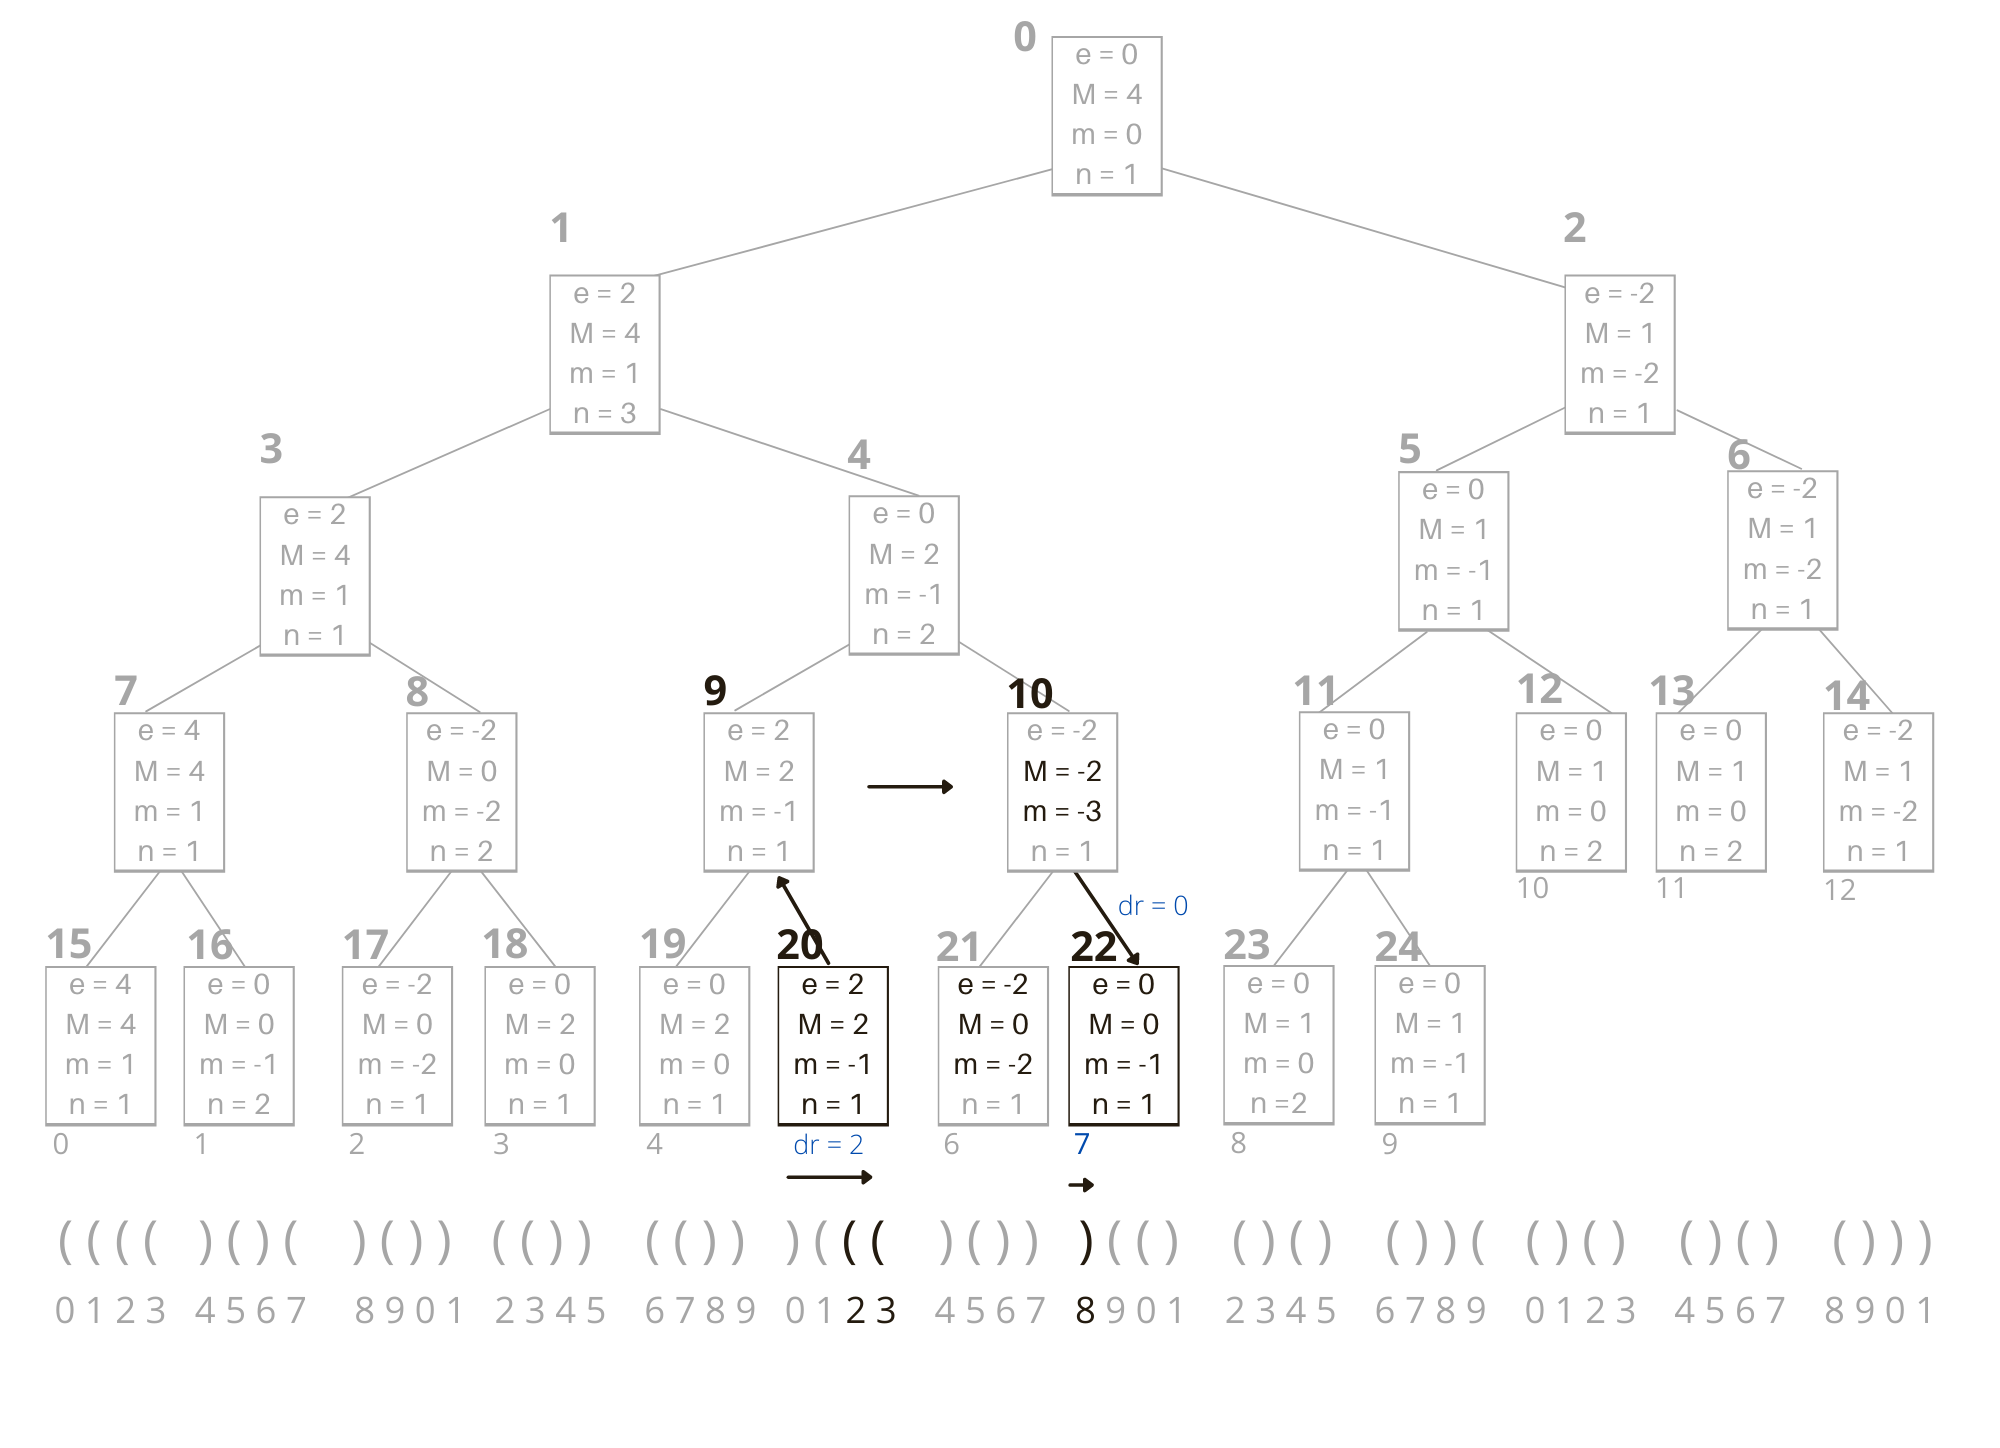
\includegraphics[width=\columnwidth]{images/rmm-tree-bin-fwdsearch.png}
             \label{fig:bin-fwdSearch}
        \end{figure}

        O processo é iniciado através da inspeção dos bits cobertos pelo nó $v=20$, os bits são inspecionados a partir da posição $i+1=22$, até chegar ao
        fim do intervalo deste nó que é $j=23$, durante esse processo de inspeção simulamos a operação de $rank_1$, guardando em $dr$ os valores computados. 
        Ao fim do intervalo, temos que $dr=2$ (como apontado na figura), como o valor buscado não foi encontrado nessa varredura inicial, precisamos aumentar o nosso espaço de busca. Fazemos isso subindo na rmM-tree através dos seus nós. 
        
        \citet{book-compact-data-structures} traz um passo interessante que otimiza a busca na árvore, essa técnica consiste em  verificar se a resposta buscada está no nó à direita do atual,evitando subidas/descidas desnecessárias na rmM-tree. Com base nessa técnica, analisamos o nó à direita de $20$, sem obter sucesso. Atualizamos  $v$ para o índice do seu nó pai $(9)$, e verificamos se os campos do nó à direita (nó $10$) adicionados de $dr$, compreendem o excesso relativo buscado $d$, ou seja $2 -3 \leq 1 \leq -2 +2$. Essa asserção é válida, portanto interrompemos a subida na árvore, e atualizamos o índice guardado em $v$ para $10$. 
        
        Iniciamos o percurso de descida na árvore. Como buscamos a posição $j$ mais à esquerda possível de $i$, verificamos primeiro se a resposta está contida no intervalo do filho esquerdo do nó $10$, o que não é verdade, em decorrência disso adicionamos à $dr$ o excesso local do nó $21$ ($dr + (-2)= 0$), e descemos então pelo filho direito de $v$, e nesse momento chegamos à um nó folha.
         
         Através desse procedimento de descida na árvore, reduzimos ao máximo o intervalo a ser inspecionado. Iniciamos então a inspeção do intervalo coberto pelo nó $22$, temos que, $dr=-1$ em $BP[28]$, que é o exceso buscado, desse modo temos que a resposta para $fwdSearch(21,-1)$ é $j=28$.
    \end{example}
    
    \begin{algorithm}[htp]
        \SetKwFunction{algo}{algo}
        \SetKwProg{myalg}{Algoritmo}{}{}
        \myalg{fwdBlock(i,d\&dr)}{
            \Input{Índice a partir do qual começamos a busca, excesso buscado, excesso computado até o momento.}
            \Output{Posição $j$ onde ocorre a resposta, ou $BP.size()$ caso a resposta não exista.}
            \vspace{.3cm}
            $fb \leftarrow \ceil{(i+1)/w}$\\
            $lb \leftarrow \ceil{(i+2)/b} \cdot (b/w)$\\
            \For{$j \leftarrow i+1$ \textbf{to} $(lb\cdot w)-1$}{
                \If{$BP[j]=1$}{$dr \leftarrow dr + 1$}
                \Else{$dr \leftarrow dr -1$}
                \If{$dr = d $}{\Return{$j$}}
            }

            \For{$p \leftarrow fb +1 $ \textbf{to} $lb$}{
                $x \leftarrow bitsRead((p-1) \cdot w)$\\
                \If{$dr + C[x].m \leq d \leq dr + C[x].M$}{\textbf{break}}
                $dr \leftarrow dr + C[x].e$
            }

            \If{$p>lb$}{
                \Return{$lb\cdot b$\tcp{dr não está no bloco subsequente}}
            }
            
            \For{$j \leftarrow (p-1) \cdot w$ \textbf{to} $(p \cdot w)-1$}{
                \If{$BP[j]=1$}{$dr \leftarrow dr + 1$}
                \Else{$dr \leftarrow dr -1$}
                \If{$dr = d $}{\Return{$j$}}
            }
            \Return{$BP.size()$}
        }
        \caption{Busca pelo excesso relativo $d$ em um nó folha.}
        \label{alg:fwdBlock}
    \end{algorithm}

    \begin{algorithm}[htp]
        \SetKwFunction{algo}{algo}
        \SetKwProg{myalg}{Algoritmo}{}{}
        \myalg{fwdSearch(i,d)}{
        \Input{Índice a partir do qual a busca deve ser feita, excesso relativo buscado.}
        \Output{Posição $j$ onde ocorre $d$, ou $BP.size()$ caso a resposta não seja encontrada.}
        \vspace{.3cm}
        $dr \leftarrow 0$\\
        $j \leftarrow fwdBlock(i,d,\&dr)$ \tcp{Algoritmo~\ref{alg:fwdBlock}}
        
        \If{$dr = d $}{\Return{$j$}}
        $l \leftarrow \floor{(i+1)/b}$\\
        $v \leftarrow leafInTree(l)$\tcp{Algoritmo~\ref{alg:folha-indice}}

        \While{$(v+1)\&(v+2)$ \textbf{and} $dr + R[v+1].m \leq d \leq dr + R[v+1].M$}{
            \If{$v$  mod  $2$}{
                $dr \leftarrow dr + R[v+1].e$
            }
            $v \leftarrow \floor{(v-1)/2}$
        }

        \If{$(v+1)\&(v+2) = 0$}{\Return{$BP.size()$}}

        $v \leftarrow v +1 $\\

        \While{$v < numberLeaves -1 $}{
            $v_l \leftarrow (2 \cdot v)+1; v_r \leftarrow v_l + 1$\\
            \If{$dr + R[v_l].m \leq d \leq dr + R[v_l].M$}{
                $v \leftarrow v_l $
            }
            \Else{
                $dr \leftarrow dr + R[v_l].e$\\
                $v \leftarrow v_r$
            }
        }

        $l \leftarrow numLeaf(v)$\tcp{Algoritmo~\ref{alg:folha-indice}}
        $j \leftarrow fwdBlock((l \cdot b)-1,d, \&dr)$\\
        \lIf{$dr = d$ }{\Return{$j$}}
        \lElse{\Return{$BP.size()$}}
        }
        \caption{Busca por um excesso relativo $d$, para um $j>i$}
        \label{alg:fwdSearch-bin}
    \end{algorithm}


    \subsection{BwdSearch}\label{sc:bwdsearch}
    Essa operação é bastante similar à \textit{fwdSearch}, portanto não entraremos em tantos detalhes. Além disso mais à frente fornecemos um exemplo que esclarece o processo para esse tipo de busca. 
    
    O ponto central de \textit{bwdSearch} é que, ao invés de realizarmos uma busca "à frente", como na operação anterior, realizamos uma busca "para trás", assim $bwdSearch$ busca por um índice $j < i$, mais à direita possível, tal que:
    $$bwdsearch(i,d) = max\{j < i | excess(j) = excess(i) - d\}$$

    Como explica \citet{book-compact-data-structures}, a relação acima impacta na nossa busca através da rmM-tree devido aos dados armazenados nas nossas estruturas serem assimétricos, o autor faz então as seguintes considerações relacionadas ao processo de inspeção na rmM-tree,  usando \textit{bwdSearch}:
    \begin{itemize}
        \item Buscamos por um excesso $j<i$, tal que:
         $$excess(j) - excess(i) = - excess(j+1,i) = d,$$ 
         isso faz com que o índice $i$ seja incluído na contagem;
        \item Queremos encontrar um índice $j$ tal que o excesso relativo computado $(dr)$, no intervalo $[i,j]$, seja igual ao excesso buscado, $d$. Mas como $j < i $ e portanto $dr = d = -excess(j+1,i)$, devemos adicionar $1$ unidade à $dr$ ao inspecionarmos um bit codificado como $0$, e diminuir $dr$ em $1$ unidade caso contrário;
        \item  Os valores de excesso são computados a partir de um processo de inspeção de bits da esquerda para a direita. A operação \textit{bwdSearch}, realiza a pesquisa por excesso da direita para a esquerda, isso implica que o excesso buscado $d$, é encontrado em um nó somente quando a asserção $dr - R[v].e + R[v].m \leq d \leq dr - R[v].e + R[v].M$ for válida.
    \end{itemize}

    Ademais, como estamos fazendo uma busca por uma posição $j<i$, mais à direita possível, durante o percurso na rmM-tree inspecionamos primeiramente o filho à direita de um nó em busca da resposta, caso não encontremos esta, avançamos no percurso através do filho à esquerdo. O Algoritmo~\ref*{alg:bwdSearch-bin} detalha mais sobre esse processo, este algoritmo invoca um método denominado \textit{bwdBlock}, este por usa vez é completamente análogo  ao Algoritmo~\ref{alg:fwdBlock} (a única ressalva é a questão de simetria discutida acima), portanto não fornecemos aqui o pseudo-código de \textit{bwdBlock}.

    O exemplo a seguir, ilustra o processo de busca pelo índice que codifica um nó, cujo parênteses de fechamento é armazenado em $BV[i]$.
    \begin{example}\label{ex:bin-bwd}
        Dado um índice $i$ em $BP$, igual à $50$, encontrar o índice $j<i$, mais à direita possível, tal que $excess(j) - excess(i) = 0$


        Como no exemplo anterior, a figura \ref{fig:bin-bwdSearch}, destaca os bits e índices dos nós inspecionados para chegar a resposta esperada.
        \begin{figure}[h!]
           \centering
             \caption[bwdSearch(50,0).]{Simulação da operação $bwdSearch(50,0)$ em uma rmM-tree binária.}
             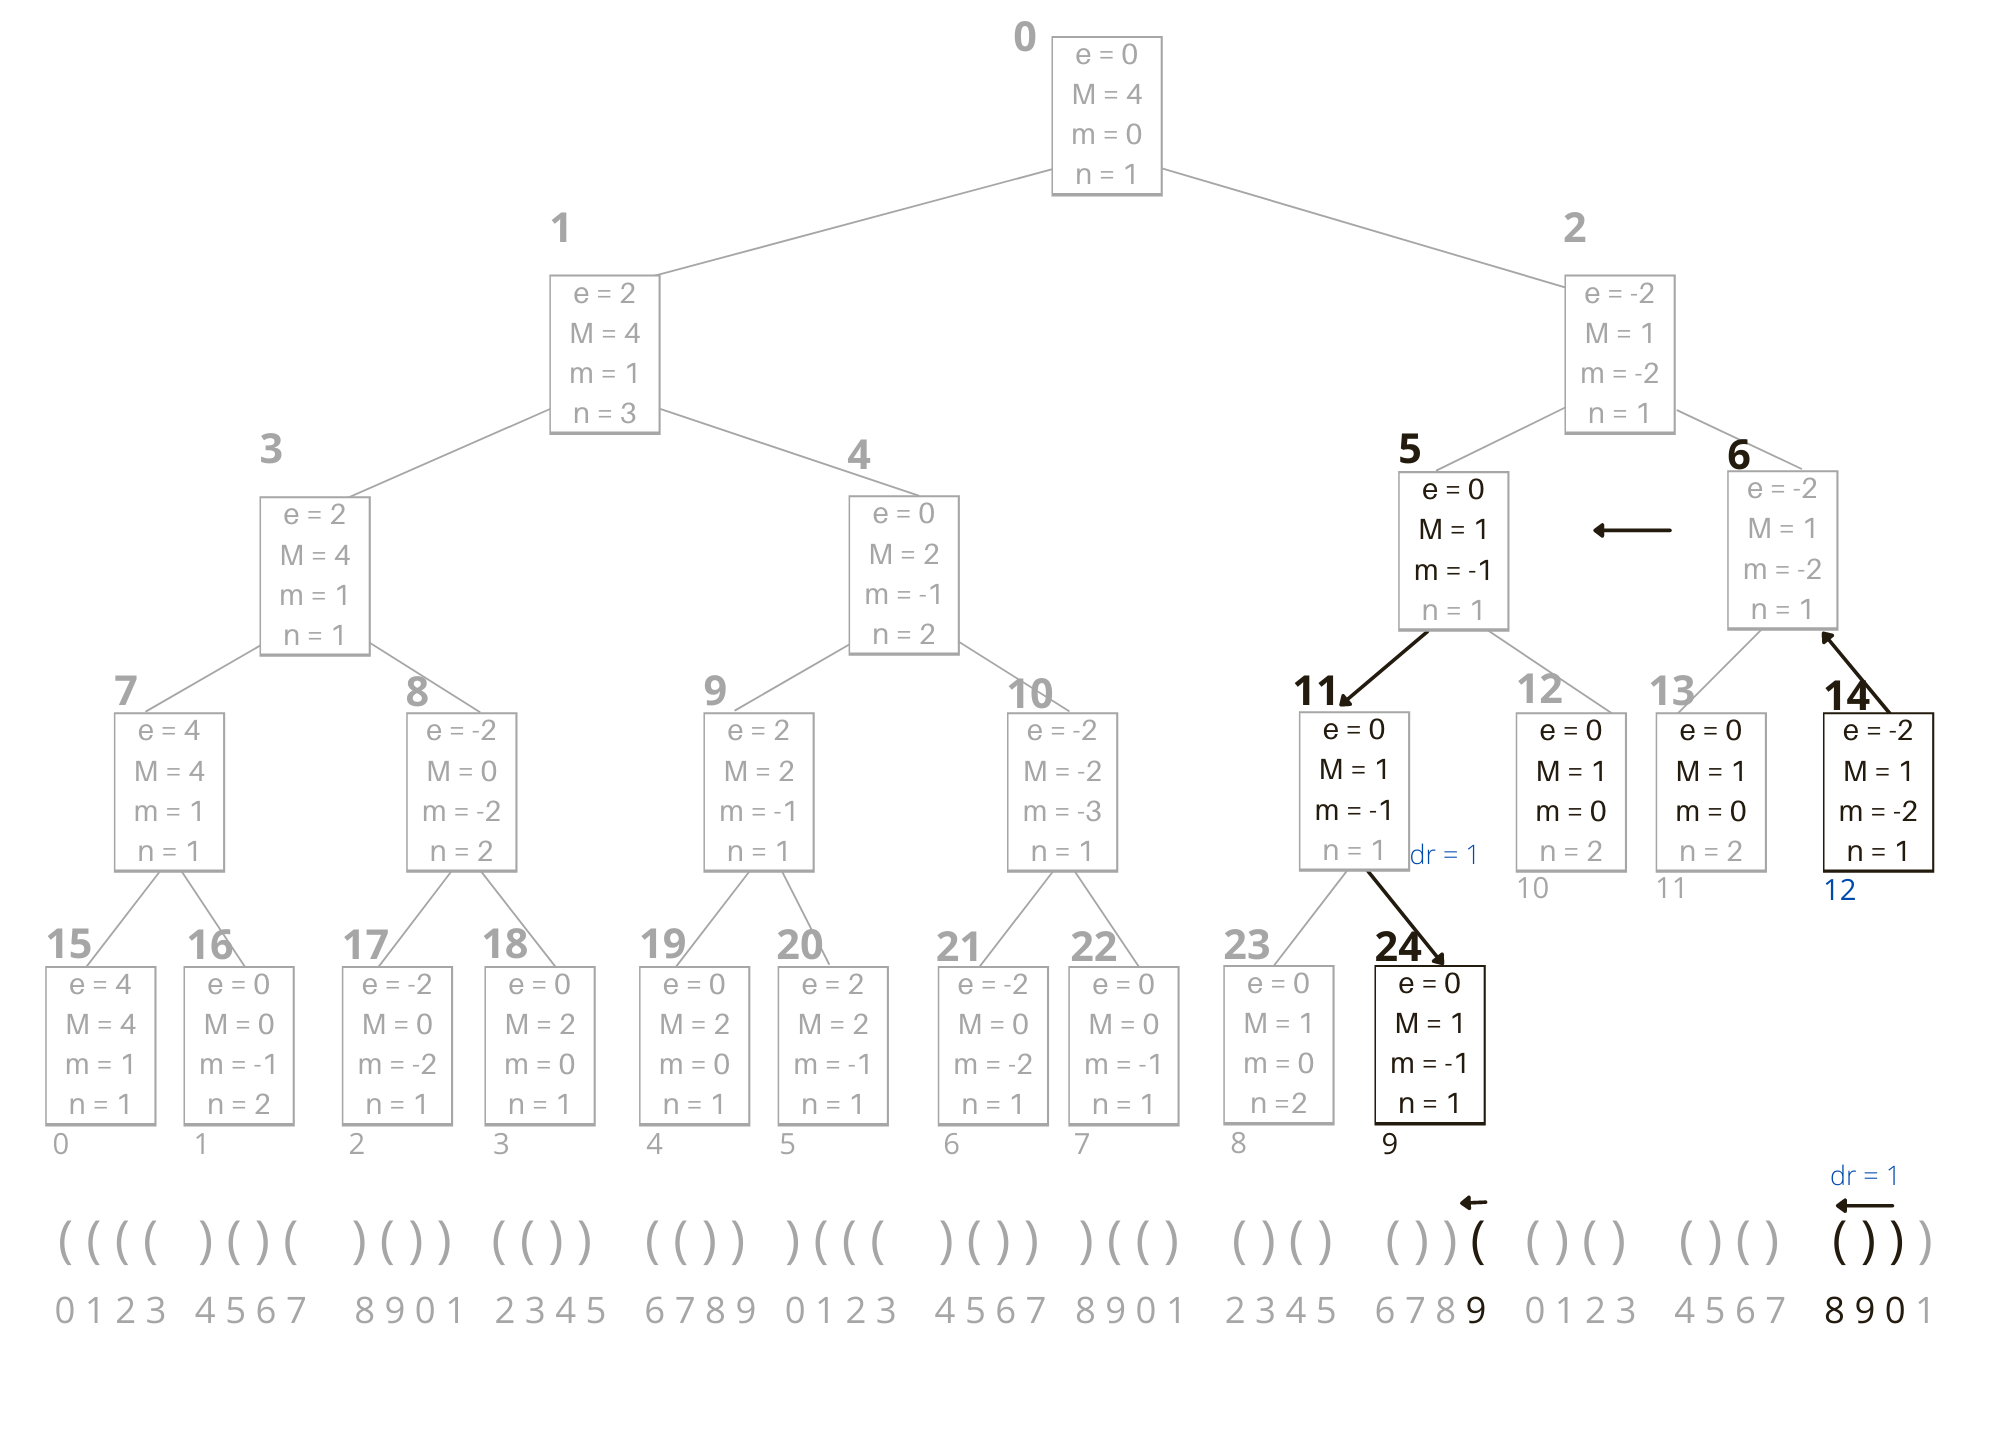
\includegraphics[width=\columnwidth]{images/rmm-tree-bin-bwdsearch.png}
             \label{fig:bin-bwdSearch}
        \end{figure}

        A nossa busca inicia a partir da análise dos bits compreendidos no intervalo da folha $12$ (nó $14$) que compreende o índice $i=50$ (reafirmamos que \textit{bwdSearch} incluí o índice $i$), ao realizarmos a inspeção desta folha, indo de $i=50$ até $j=49$, temos um excesso relativo computado até o momento $(dr)$ igual à $1$. 
        
        Como o excesso é diferente do valor buscado precisamos usar os nós da rmM-tree para encontrar a resposta. Usamos a mesma técnica de otimização de \textit{fwdSearch} e verificamos se $d$ está compreendido nos intervalos de excesso mínimo e máximo do nó à esquerda de $v=14$. A resposta não é encontada no nó $13$, e assim iniciamos o processo de subida na árvore, atualizando o valor de $v$ para $6$.
        
        Analisamos o nó à esquerda de $v=6$, verificando a asserção\footnote{$dr - R[v].e + R[v].m \leq d \leq dr - R[v].e + R[v].m$.} $ 1 -0 -1 \leq 0 \leq 1 -0 +1$. Como a comparação é verdadeira interrompemos o processo de subida na árvore, e atualizamos o valor de $v$ para o nó que contém a resposta.
        
        Iniciamos a descida na árvore, pelo nó $v=5$: verificamos se $d$ está contido nos registros de excesso do filho direito (nó $12$) de $v$, como a busca no filho direito falha, significa que a resposta está no intervalo do filho esquerdo, desse modo atualizamos o índice de $v$ para $11$.

        Continuamos o processo de descida na árvore através do nó $11$, analisamos primeiro o filho direito de $11$ e verificamos que $d$ está contido nos intervalos de excesso deste nó, avançamos para o nó $24$. Como chegamos à um nó folha, interrompemos a busca através dos nós da rmM-tree, e iniciamos uma busca no vetor $BP$. Ao analisarmos o índice $j=39$, $dr$ passa a valer $0$, e portanto a busca pelo excesso $d$ através de \textit{bwdSearch} é concluída, retornando $j=39$. 
    \end{example}

    \begin{algorithm}[htp]
        \SetKwFunction{algo}{algo}
        \SetKwProg{myalg}{Algoritmo}{}{}
        \myalg{bwdSearch(i,d)}{
        \Input{Índice $i$ a partir do qual a busca deve ser feita, excesso relativo $d$ desejado}
        \Output{Posição $j$ onde ocorre o $d$, ou $-1$ caso a resposta não seja encontrada}
        \vspace{.3cm}
        $dr \leftarrow 0$\\
        $j \leftarrow bwdBlock(i,d,\&dr)$ \tcp{Análogo ao algoritmo~\ref{alg:fwdBlock}}
        
        \If{$dr = d $}{\Return{$j$}}
        $l \leftarrow \floor{i/b}$\\
        $v \leftarrow leafInTree(l)$\\

        \While{$(v+1)\& v$ \textbf{and} $dr - R[v-1].e + R[v-1].m \leq d \leq dr - R[v-1].e + R[v-1].M$}{
            \If{$v$ mod $2 = 0$}{
                $dr \leftarrow dr - R[v-1].e$
            }
            $v \leftarrow \floor{(v-1)/2}$
        }

        \If{$(v+1)\&v = 0$}{\Return{$-1$}}

        $v \leftarrow v - 1 $\\

        \While{$v < numberLeaves -1 $}{
            $v_l \leftarrow (2 \cdot v)+1; v_r \leftarrow v_l + 1$\\
            \If{$dr - R[v_r].e + R[v_r].m \leq d \leq dr - R[v_r].e + R[v_r].M$}{
                $v \leftarrow v_r$
            }
            \Else{
                $dr \leftarrow dr - R[v_r].e$\\
                $v \leftarrow v_l$
            }
        }

        $l \leftarrow numLeaf(v)$\\
        $j \leftarrow bwdBlock(((l+1)\cdot b)-1,d, \&dr)$\\
        \If{$dr = d$ }{\Return{$j$}}
        \Else{\Return{$-1$}}
        }
        \caption{Busca por um excesso relativo $d$, para um $j<i$. }
        \label{alg:bwdSearch-bin}
    \end{algorithm}

    \subsection{MinExcess}
    Esta é outra importante operação suportada pela rmM-tree. A partir dela podemos obter informações importantes sobre o nosso conjunto de dados, como o menor ancestral comum entre dois nós.
    
    
    O objetivo da \textit{minExcess}, é encontrar o excesso mínimo dentro de um intervalo $[i, j]$. Assim como para as outras operações, esta, inicia-se a partir da inspeção do nó folha que contém o índice $i$. Para \textit{minExcess}, a folha é analisada a partir do índice $i$ até chegarmos ao seu limite, ou até visitarmos o índice $j$, caso este esteja engolobado no intervalo da folha de $i$. 

    Durante a análise da folha, a cada bit lido, guardamos em uma varíavel $d$ o valor do excesso relativo computado até o momento, verificamos também se este excesso é o menor até o momento.

    Terminando a inspeção da folha que contém $i$, caso $j$ não esteja contido nela, iniciamos o processo de subida na árvore (caso $j$ esteja contido, a busca é encerrada, e é retornado o menor excesso computado no intervalo analisado). Durante o percurso pela rmM-tree verificamos se os registros de excesso mínimo salvo em cada nó é menor que o excesso mínimo computado até o momento, em caso afirmativo, atualizamos o excesso mínimo computado até o momento. E independente da resposta, atualizamos o valor do excesso relativo $d$.

    Ressalta-se que o percurso em árvore para esta operação é idêntico ao percurso em árvore em \textit{fwdSearch}, sendo interrompido no momento em que estamos prestes a inspecionar um nó $v$, que seja ancestral do nó folha cujo intervalo engloba o índice $j$.

    Para tanto, precisamos de algumas informações, trazidas por \citet{book-compact-data-structures}, que são:
    \begin{itemize}
        \item A profundidade de qualquer nó em $R[v]$ é dada por $\floor{\log (v + 1 )}$;
        \item O pai de um nó, é dado por $\floor{(v-1)/2}$;
        \item À medida que avançamos da esquerda para a direita na rmM-tree, seguindo a abordagem bottom-up, um nó $u$ é dito ancestral de um nó $v$, se a asserção abaixo for válida,
        $$\floor{(v-1)/2^{\floor{\log (v+1)} - \floor{\log (u+1)}}} = u$$
        \item Conforme explica o autor, durante o percurso na árvore, a asserção acima pode ter um comportamento inesperado quando  $u$ for um nó folha, e tiver uma profundidade maior que a do nó alvo (a folha que contém o índice $j$). \citet{book-compact-data-structures} explica que isso pode ocorrer quando o número de folhas não for uma potência de $2$. 
        Para suprir esse problema devemos criar outro critério de continuação de subida na árvore, que é verificar se o índice do nó inspecionado é ou não, maior do que o índice do nó alvo, em caso afirmativo a busca prossegue com a subida na árvore. Desse modo, caso o índice do nó $u$ não for maior do que o índice do nó alvo, e a asserção do tópico anterior for verdadeira, a busca é interrompida.
    \end{itemize}


    Ao encontrarmos o ancestral do nó alvo, interrompemos a subida na rmM-tree, e começamos o processo de descida a partir deste ancestral. O percurso de descida ocorre de modo similar ao da operação \textit{fwdSearch}, verificamos primeiro se o filho  esquerdo do nó visitado é ancestral do nó alvo, em caso positivo descemos na rmM-tree pelo filho esquerdo de $v$.  Em caso negativo, usamos os registros de excesso deste nó para verificar se existe um excesso mínimo menor que o computado até o momento, atualizando esse valor conforme a resposta que obtivermos; e então atualizamos o valor de $v$ para o índice do filho à direita deste nó. 

    Repetimos todo esse processo até que cheguemos a um nó folha. Tendo atingido um nó folha, realizamos a inspeção do mesmo, do seu início, até a posição $j$, verificando se os valores de excesso deste intervalo são inferior ao excesso mínimo computado até o momento. Ao término dessa inspeção, temos o excesso mínimo em $BP[i,j]$.


    O exemplo a seguir ilustra como a busca pelo excesso mínimo se dá através da operação \textit{minExcess}.
    \begin{example}
        Dado o intervalo $BP[18,39]$, retornar o menor excesso.

       \begin{figure}[!ht]
           \centering
             \caption[minExcess(18,39).]{Simulação da operação $minExcess(18,39)$ em uma rmM-tree binária.}
             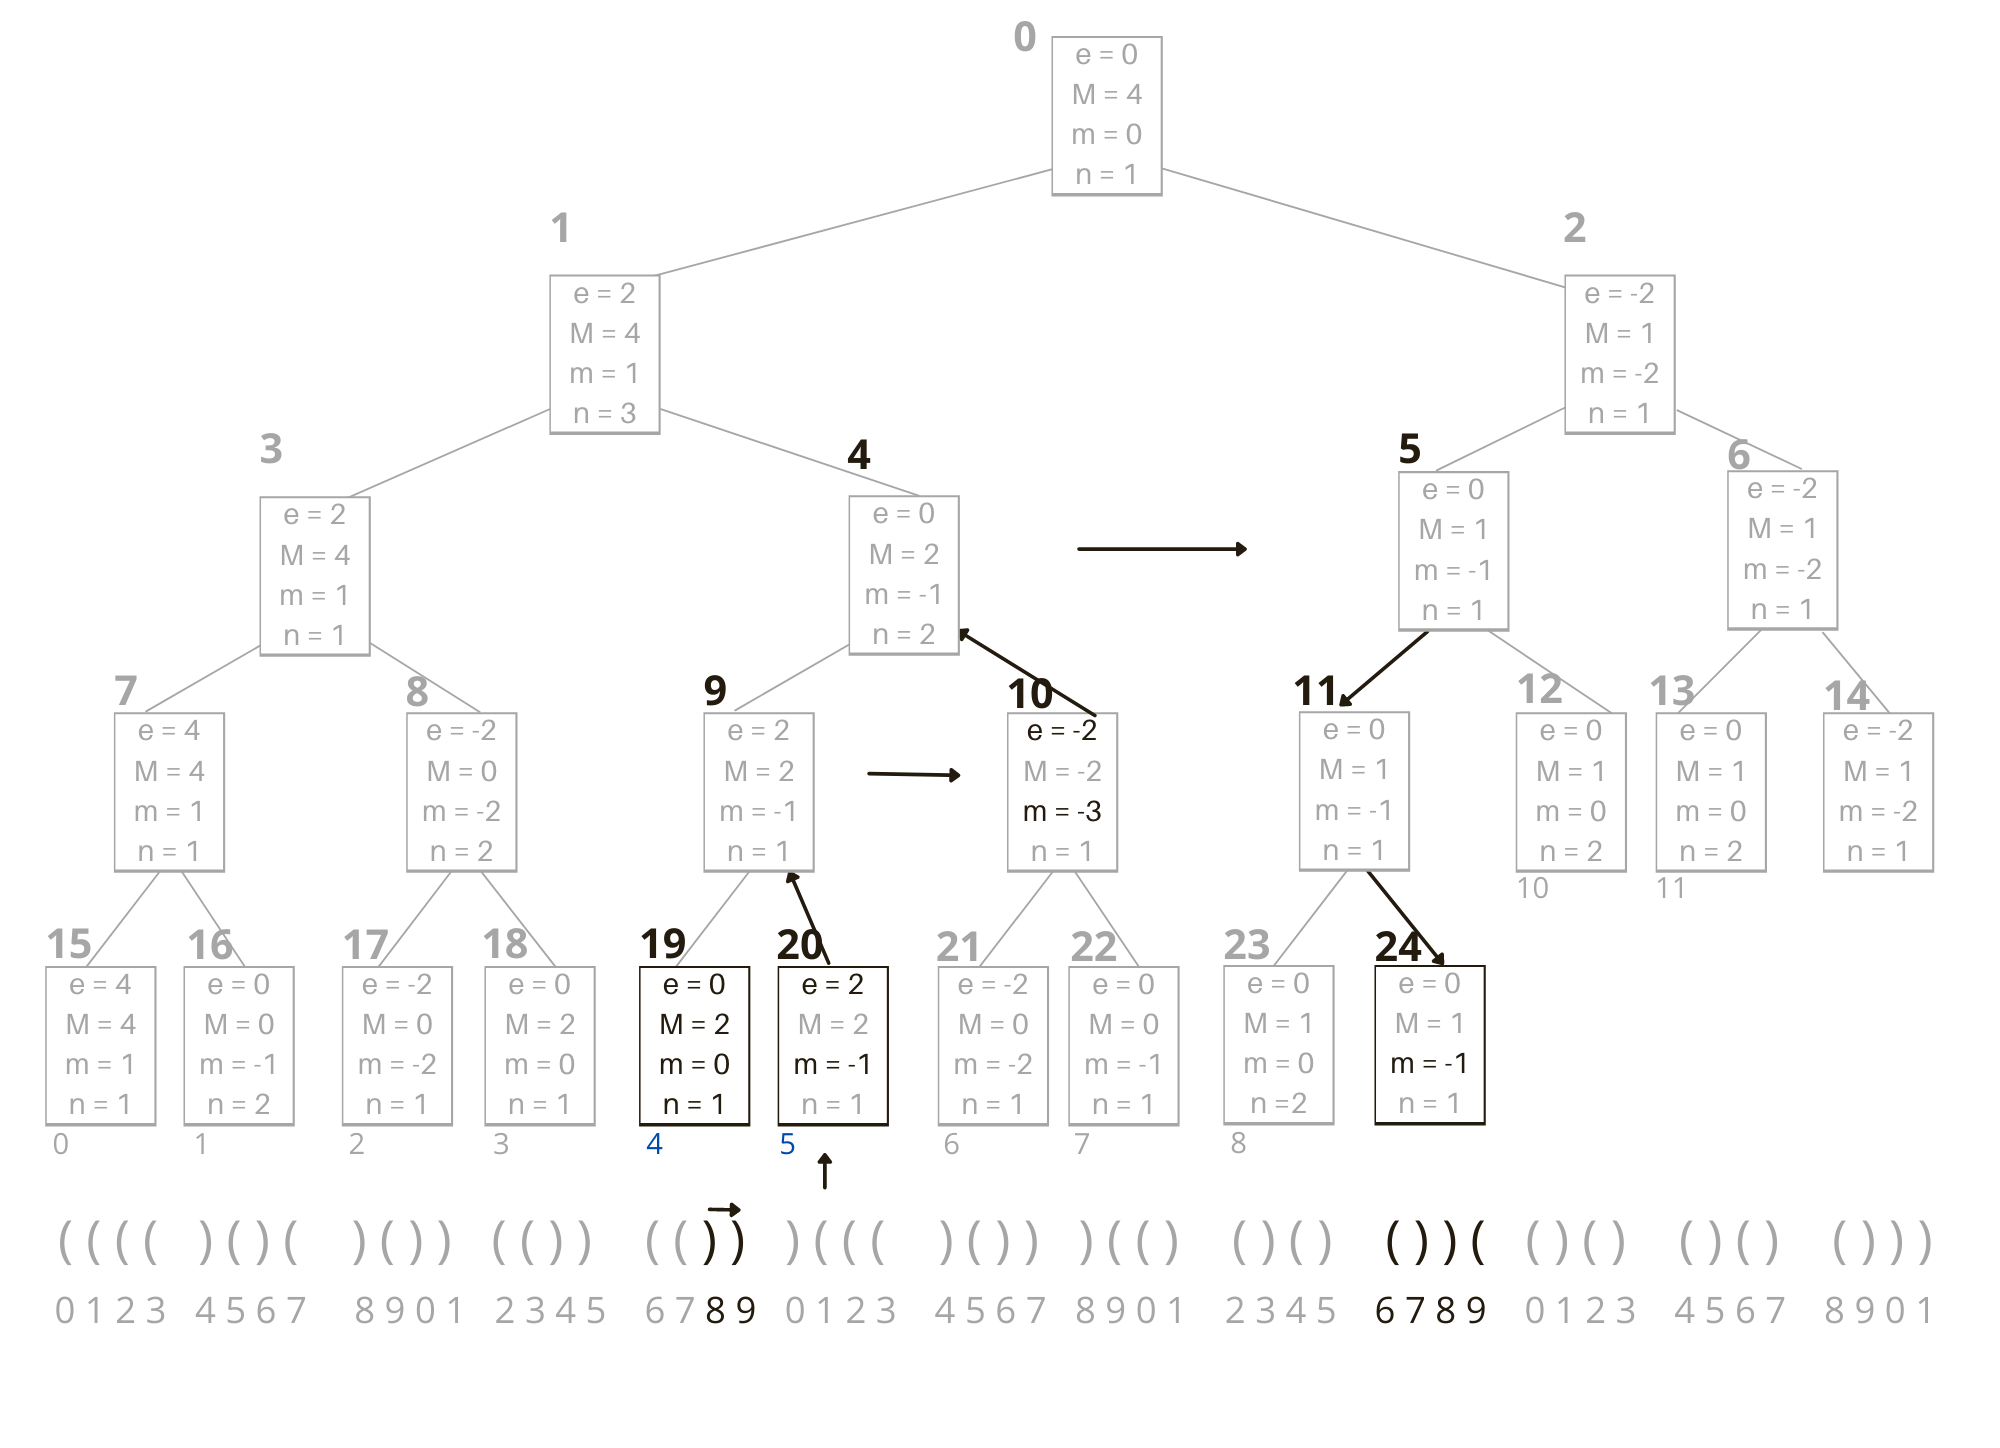
\includegraphics[width=\columnwidth]{images/rmm-tree-bin-minexcess.png}
             \label{fig:bin-minexcess}
        \end{figure}

        Primeiro fazemos a análise da folha que contém o índice $i$, realizamos uma varredura parcial do intervalo da folha $4$ (nó $19$), indo de $i=18$ até $p=19$, nesse momento temos que o excesso mínimo ($m$) e o excesso local ($d$) computado até o momento, valem $-2$.

        Como $j$ não está compreendido no intervalo da folha $4$, precisamos identificar o nó folha cujo o intervalo compreende $j$, este nó é dado por $x=24$. Verificamos se o excessmo mínimo no nó à direita de $v=19$, é menor que o excesso computado até o momento, como a asserção é válida $-2 -1 < -2$ (por $d + R[20].m < d]$), atualizamos o valor de $m$ para $-3$, e o valor de $d$ para $0$.

        Como $j$ não está compreendido no irmão à direita de $v$, iniciamos o percurso de subida na árvore através nó $9$. Analisamos se o nó à direita de $v$ é ancestral do nó alvo, e obtivemos que o nó $10$ não é ancestral de $x$, com base nos registros do nó $10$ atualizamos o valor de $d$ para $-2$, e subimos na árvore através do nó $4$. Novamente, verificamos se o nó à direita ($5$) do nó atual é ancestral do nó $x=24$, e nesse momento
        temos uma afirmação verdadeira. 
        
        Tendo achado o nó ancestral de $x$, interrompemos o processo de subida na árvore, e iniciamos o processo de descida  a partir do nó $v=5$. Ao analisarmos os filhos de $v$, temos que o seu filho esquerdo (nó $11$) é ancestral do nó $24$, então atualizamos o valor de $v$ para $11$, e verificamos os filhos do mesmo. Temos nesse momento que o filho esquerdo de $v$ (nó $23$) não é ancestral do nó alvo, desse modo atualizamos o valor de $v$, para o índice do seu filho à direita, que é o próprio nó alvo.

        Como chegamos à um nó folha, interropemos a verificação dos nós da rmM-tree, e iniciamos a verficiação do excesso mínimo na folha $9$ (nó $24$), ao pecorrer está folha o valor do excesso mínimo computado até o momento não é alterado, e portanto $BP[18,39].m=-3$.
    \end{example}

        
        Uma outra variação dessa operação é a \textit{maxExcess}, o processo para responder está é completamente análogo ao descrito acima, mudando apenas os registros da rmM-tree analisados(ao invés de verificarmos o excesso mínimo, verificamos o excesso máximo).

    \subsection{MinCount e MinSelectExcess}
    Essas operações possuem bastate similaridade entre si, e também são análogas à \textit{minExcess}, portanto não entraremos em  detalhes sobre as duas. 
    
    De modo geral, o objetivo da operação \textit{minCount} é computar o número de vezes que o excesso mínimo aparece no intervalo $BP[i,j]$, ao passo que a operação \textit{minSelectExcess}, 
    objetiva encontrar o índice dentro do intervalo $[i,j]$, onde ocorre a $t-$ésima ocorrência do excesso mínimo computado neste mesmo intervalo. 
    Observe que para ambas as operações, é necessário primeiro computar o excesso mínimo dentro do intervalo fornecido, para tanto, podemos fazer uma chamada a função \textit{minExcess}, 
    e então pecorrer a rmM-tree em busca da resposta esperada para cada operação. 
    
    Para realizar a operação \textit{minCount}, cria-se um acumulador que é incrementado através do registro $n$, da rmM-tree, sempre que passarmos por um nó cujo o valor de excesso mínimo for igual ao excesso computado por \textit{minExcess}. 

    A operação \textit{minSelectExcess} é análoga, para ela, pode-se criar um acumulador que recebe o valor $t$, passado para a função, e assim ao visitar um nó cujo o valor de excesso mínimo é igual ao valor computado por \textit{minExcess}, subtraímos do acumulador  o valor armazenado em $n$, a resposta nesse caso é encontrada quando o acumulador atinge a marca menor ou igual à $0$. Para ambas as operações, o processo de subida e descida na árvore se dá de igual modo ao mostrado em \textit{minExcess}.


    Essas são as únicas operações que usam o registro $n$ da rmM-tree, portanto não há necessidade de fazer a computação deste, caso o objetivo da sua estrutura não englobe uma destas operações ou suas derivadas.

    \subsection{Derivadas}
    Esta seção demonstra como diversas operações sobre a rmM-tree podem ser escritas de modo eficiente a partir das operações descritas anteriormente.

    \begin{itemize}
        \item \textbf{rmq}: busca pela primeira posição onde ocorre o excesso mínimo computado dentro do intervalo  $BP[i,j]$. Ou seja:
            $$rmq(i,j) =\min \{ \argmin\{excess(p) | i \leq p \leq j\}\} $$
    
        Para à responder esta operação, podemos computar primeiro o exesso mínimo dentro do intervalo $i,j$, e em seguida realizar uma busca a partir de $i$.
        Temos assim:
        $$rmq(i,j) = fwdSearch(i-1,minExcess(i,j))$$
        Repare que o primeiro parâmetro  em \textit{fwdSearch} é subtraído em $1$, isso acontece porque o intervalo da busca  de \textit{fwdSearch} é aberto, ou seja, não incluí o índice $i$ passado nas buscas, ao passo que o intervalo de \textit{rmq} é fechado, incluindo $i$ e  $j$ nas buscas. 
    
        \item \textbf{rMq}: similar a operação anterior, \textit{rMq}, busca a posição mais à esquerda de $i$ onde ocorre o excesso máximo computado em $i,j$. Ou seja:
        $$rMq(i,j) =\max\{ \argmax\{excess(p) | i \leq p \leq j\}\} $$   
        
        Assim:
            $$rMq(i,j) = fwdSearch(i-1, maxExcess(i,j))$$


        \item \textbf{findClose}: essa operação recebe como parâmetro um índice $i$, correspondente à um nó, isto é, a um parênteses de abertura, e a partir da operação \textit{fwdSearch}, busca o parênteses de fechamento correspondente. A operação \textit{fwdSearch} pecorrerá o vetor de bits e rmM-tree a partir de $i+1$ até que encontre o índice $j > i $, tal que 
        $excess(j) - excess(i+1) = -1 $.  Assim:
        $$findClose(i) = fwdSearch(i,-1)$$
            
        \item \textbf{findOpen}:  dado um índice, tal que $BP[i]=0$, \textit{findOpen}, faz uma busca por um $j < i $ tal que $excess(j) - excess(i) = 0$ e $excess(j)+1=1$. 
        Isso nos dá:
        $$findOpen(i) = bwdSearch(i,0)+1$$
        
        \item \textbf{enclose}: dado um índice $i$, que indica a codificação de um nó $x$, \textit{enclose} retornará o pai do nó $x$, usando a operação \textit{bwdSearch} para encontrar a posição $j<i$ mais à direita de $i$, tal que $excess(j) - 2 = 1$. Ou seja:
        $$enclose(i) = bwdSearch(i,-2) + 1$$

        \item  \textbf{levelAncestor}: essa operação buscará pelo nó $y$ que que seja ancestral e esteja $d$ níveis acima de um nó $x$. Para tanto podemos usar a operação \textit{bwdSearch}. Por questões de simetria, já discutidas anteriormente, devemos passar o valor de $d$ como negativo em \textit{bwdSearch}, e assim temos:
        $$levelAncestor(x,d) = bwdSearch(x,-d-1)+1$$
        
        \item \textbf{isAncestor}: essa função tem por objetivo verificar se um nó $x$ é ancestral de um nó $y$, para tanto, basta verificar se $y$ está contido na hierarquia de $x$. Podemos usar \textit{findClose}, como mostrado abaixo:
        $$ isAncestor(x,y) = (x < y  \mbox{ and }  y < findClose(x))$$
        
        \item \textbf{parent}: dado um índice $i$, correspondente ao bit que codifica um nó $x$, \textit{parent} busca através de \textit{enclose} o índice em $BP$ do nó que codifica
        o nó pai de $x$:
        $$parent(i) = enclose(i)$$
        
        \item \textbf{lca}: busca o menor ancestral comum entre dois nós, codificados nos índices $i$ e $j$. Existem 3 possibilidades de retorno para \textit{lca}, são eles:
        $$lca(i,j) =
               \begin{cases}
                     i,  \mbox{se } isancestor(i,j); \\
                    j, \mbox{se } isancestor(j,i); \\
                    parent(rmq(i ,j)+1)
               \end{cases}
        $$

        \item \textbf{deepestNode}: dado um nó em $BP$, \textit{deepestNode} retorna o descendente com maior profundidade deste nó (localizado mais à esquerda possível). Sabemos que para calcular o maior excesso possível a partir de $i$ podemos usar a operação \textit{maxExcess}. Como esse excesso deve estar limitado ao escopo do nó codificado em $i$, temos a seguinte relação:

        $$deepestNode(i) = rMq(i, findClose(i))$$

        A operação $rMq$ é usada aqui para invocar \textit{maxExcess} e em seguida retornar a posição exata onde ocorre o excesso computado.

        \item \textbf{degree}: esta operação contabiliza o número de filhos de um nó codificado em $i$. Como a sequência que representa a nossa ávore de entrada é balanceada, sabemos que dentro do intervalo (aberto) de hierarquia de um nó, atingimos o excesso mínimo sempre que finalizamos a codificação de um de seus nós filhos. Levando isso em consideração, podemos calcular \textit{degree} do seguinte modo:
        $$degree(i) = minCount(i+1, findClose(i)-1)$$
        
        \item \textbf{childRank}: dado um índice $i$, \textit{childRank}, contabiliza o número de irmãos que o nó codificado em $i$ possuí à sua esquerda. Tendo as operações definidas anteriormente, podemos responder à esta operação conforme mostrado abaixo:
        $$
               childRank(i) = minCount(parent(i)+1, i) +1
        $$
        
        \item \textbf{nextSibling}: dado um nó codificado em $i$, \textit{nextSibling} busca pelo irmão localizado no mesmo nível do nó $i$, codificado em $j$, tal que $j>i$.
        $$nextSibling(i) = findClose(i) +1$$
        
        \item \textbf{prevSibling}: análaga a \textit{nextSibling}, esta operação busca pelo irmão imediatamente à esquerda do nó codificado por $i$, em seu mesmo nível. Ou seja:
        $$prevSibling(i) = findOpen(i-1)$$
        
        \item \textbf{child}: dado um índice $i$ que codifica um nó, \textit{child} calcula a posição em $BP$ onde ocorre a codificação do $t$-ésimo filho de $i$  -- ou seja essa operação busca pelo índice $j$ onde acontece a $t$-ésima ocorrência do excesso mínimo dentro do intervalo do nó $i$ --  desse modo, podemos escrever
        \textit{child} em função de \textit{findClose} e \text{minSelectExcess}:
        $$p = findClose(i)$$
        $$child(i) = minSelectExcess(i+1,p-1,t-1) + 1 $$

        \item \textbf{lastChild}: busca pelo último filho de um nó codificado em um índice $i$:
        $$lastChild(i) = findOpen(findClose(i)-1)$$
        
        \item  \textbf{subtreeSize}: calcula o tamanho da subárvore enraízada no nó $i$, para tanto, basta realizar uma contagem dos nós codificados no intervalo do 
        nó $i$, ou seja:
        $$subtreeSize(i)= \floor{(findclose(i) - i + 1)/2}$$
        
        \item \textbf{levelNext}: busca o nó a direita do nó codificado por $i$, em seu mesmo nível:
        $$levelNext(i) = fwdSearch(findClose(i),1)$$
        
        \item \textbf{levelPrev}: análaga a \textit{levelNext}, esta função busca pelo primeiro nó imediatamente à esquerda do nó codificado em $i$ e que possuí a mesma profundidade deste. Como estamos falando de uma busca à esquerda de um índice, usamos \textit{bwdSearch} para realizar está operação:
        $$levelPrev(i) = findOpen(bwdSearch(i,0)+1)$$
        
        \item \textbf{levelLeftMost}: busca pelo nó mais à esquerda da raíz, com profundidade $d$, assim:
        $$levelLeftMost(d) = fwdSearch(0,d-1)$$
        
        \item \textbf{levelRightMost}: usando como referência a raíz, busca pelo nó mais à direita, cuja profundidade é igual  à $d$:
        $$levelRightMost(d) = findOpen(bwdSearch(BP.size()-1,d)+1)$$
    \end{itemize}
    
    Algumas das operações a seguir, além das nossas primitivas, usam em seu escopo as operações suportadas pela estrutura de vetores de bits (algumas, como o caso de \textit{depth} usam apenas estás últimas). Isso nos mostra também a importância do cuidado ao escolhermos uma estrutura de suporte apropriada afim de acelerar nossas operações.
        \begin{itemize}
            \item \textbf{firstChild}: retorna o primeiro filho do nó codificado por $i$, logo:
            $$firstChild(i) = i +1$$
            \item \textbf{isLeaf}: dado um nó codficiado em $i$, verifica se este é um nó folha ou não, essa é uma das operações mais simples da nossa estrutura e necessista apenas de 2 comparações, veja abaixo:
            $$isLeaf(i) = (BP[i] = 1 \land BP[i+1]=0)$$
            \item \textbf{depth}: computa a profundidade de um nó codficado por $i$, para tanto basta verificar o exesso em $BP[0,i]$, ou seja:
            $$depth(i) = excess(i)$$
            \item \textbf{leafRank}: contabiliza a quantidade de folhas existente em um intervalo que vai de $0$ à $i$. Em nossa implementação, usamos a operação \textit{rank},
            suportada pela estrutura de vetores de bits. Assim, basta buscar a quantidade de ocorrêncas de bits $1$ seguidos por bit $0's$.
            $$leafRank(i) = rank_{10}(i)$$
            \item \textbf{leafSelect}: esta operação nos permite buscar pela $i-$ésima folha em $BP$, para essa operação buscamos pela $i-$ésima ocorrência do padrão $10$:
            $$leafSelect(i) = select_{10}(i)$$
            \item \textbf{leftMostLeaf}: retorna a folha mais à esquerda da subárvore com raíz em $i$.
            $$leftMostLeaf(i) = leafSelect(leafRank(i-1)+1)$$
            \item  \textbf{rightMostLeaf}: retorna a folha mais à direita da subárvore com raíz em $i$
            $$rightMostLeaf(i) = leafSelect(leafRank(findClose(i)))$$
            \item \textbf{preRank}: retorna o índice do nó na árvore de entrada correspondente à $i$,  considerando um percurso em pré-ordem.
            $$preRank(i) = rank_1(i)$$
            \item \textbf{postRank}: retorna o índice do nó na árvore de entrada correspondente à $i$,  considerando um percurso em pós-ordem.
            $$postRank(i) = rank_0(findClose(i))$$
            \item \textbf{preSelect}: retorna a posição em $BP$, do $i$-ésimo nó na árvore de entrada, considerando um percurso em pré-ordem:
            $$preSelect(i) = select_1(i)$$
            \item \textbf{postSelect}: retorna a posição em $BP$, do $i$-ésimo nó na árvore de entrada, considerando um percurso em pós-ordem:
            $$postSelect(i) = findOpen(select_0(i))$$
        \end{itemize} 

%a tabela~\ref{tbl:classicOperations-rmm-tree}  mostra as operações suportadas por essa estrutura.
\begin{table}[h!]
	\centering
	\caption[Operações sobre a RMM-tree clássica]{Operações suportadas pela rmM-tree bináriaW}
	\label{tbl:classicOperations-rmm-tree}
	\rowcolors{2}{lightgray!30}{white}
	\resizebox{\columnwidth}{!}{
	\begin{tabular}{ll}
	\toprule
	\textbf{Operação} & \textbf{Retorno} \\
	\toprule
    
	fwdSearch(i,d)  & Índice $j$, tal que $excess(j) = excess(i) + d$\\
	bwdSearch(i,d)  & Índice $j$, tal que $excess(j+1,i) = -d$\\
	minExcess(i,j) / maxExcess(i,j)  & Excesso mínimo/máximo em $i,j$\\
	minCount(i,j)  & Número de vezes que o excesso mínimo aparece em $i,j$\\
	minSelectExcess(i,j,t)  & Índice da $t-$ésima ocorrência do excesso mínimo em um intervalo\\
	enclose(i) & Posição do parênteses de abertura que envolve  $BV[i]$  \\
	rmq(i,j) / rMq(i,j) & $p>=i$ mais à esquerda de $i$, onde ocorre o excesso mínimo/máximo do intervalo dado \\
	rank$_1$(i) / rank$_0$(i) & Número de parênteses abrindo/fechando em $BV[0,i]$ \\
    select$_1$(i) / select$_0$(i) & Posição do i-ésimo parênteses de abertura/fechamento\\
    preRank(i)/postRank(i) & rank de $i$ calculado a partir de um percurso \textit{preorder \mbox{ ou } postorder} \\
    preSelect(i)/postSelect(i) & retorna o nó com \textit{preorder/postorder} $i$\\
    isLeaf(i) & Verifica se $BV[i]$ codifica uma folha \\
    isAncestor(i,j) & Verifica se o nó codificado em $i$ é ancestral de $j$ \\
    depth(i) & Profundidade do nó $i$ \\
    parent(i) & Obtém o pai do nó $i$ \\
    firstChild(i) / lastChild(i) & Retorna o primeiro/último filho do nó codficiado em $BV[i]$ \\
    child(i,t)&$t-$ésimo filho do nó codificado em $i$\\
    nextSibling(i) / prevSibling(i) & Primeiro irmão à direita/esquerda de $i$ \\
    subtreeSize(i) & Número de nós enraízados na subárvore de $i$ \\
    levelAncestor(i,d) & Ancestral $j$ de $i$ tal que $depth(j) = depth(i) - d$\\
    levelNext(i) / levelPrev(i) & Nó à direita/esquerda de $i$ com a mesma profundidade de $i$.\\
    levelLeftMost(d) / levelRightMost(d) &Nó mais à esquerda/direita, com profundidade d.\\
    lca(i,j)&Menor ancestral comum dos nós codificados em $i$ e $j$\\
    deepestNode(i)&Nó mais profundo de $i$ (mais à direita possível)\\
    degree(i)&Número de filhos do nó $i$ \\
    childRank(i)&Número de irmãos à esquerda do nó codificado em $i$\\
    leafRank(i)& Número de folhas à esquerda da folha codificada em $i$ \\
    leafSelect(i)& $i-$ésima folha em $BV[0,size-1]$ \\
    leftMostLeaf(i)& folha codificada em $j$, mais à direita de $i$, tal que $j<i$\\
    rightMostLeaf(i)& folha codificada em $j$, mais à direita possível, tal que $j \leq i$\\
	\bottomrule
	\end{tabular}
	}
\end{table}



\section{rmM-tree k-ária}
%A redução do preço e o aumento da capacidade da memória principal possibilitam que grandes conjuntos de dados residam na memória principal \citet{paper-effect-node-size-cache-b-trees},
%onde o tempo para acessar um dado é menor. 

Como vimos, o uso das estruturas de dados sucintas permitem que grandes conjuntos de dados residam e sejam operados na memória principal.  \citet{paper-effect-node-size-cache-b-trees} nos mostram que, com os  dados residindo na memória RAM, um novo gargalo é criado, que surge em decorrência do atraso ao buscarmos na memória principal um dado que não se encontra em cache. 

Quando uma referência de memória é satisfeita pela cache, estas prosseguem na velocidade do processador, as referências insatisfeitas incorrem em uma penalidade no tempo de execução da busca, devido a necessidade de buscar o bloco correspondente na memória principal. Conforme citam \citet{paper-effect-node-size-cache-b-trees} o tempo gasto para buscar um dado em cache é de uma à duas ordens de magnitude menor do que a latência para a recuperação de dados na memória principal. Desse modo, a utilização inadequada da cache pode fazer com que a latência da memória se torne um gargalo crescente de desempenho, impedindo que as aplicações se beneficiem das crescentes melhorias de hardware \citep{paper-making-btree-cache}.
 
\citet{paper-effect-node-size-cache-b-trees} realizaram um estudo sobre o efeito da maximização da quantidade de informações relevantes armazenada em um nó de uma árvore denominada \textit{Cache-Sensitive Search Trees (CSS-tree)}, uma estrutura de índice consciente de cache, que possuí um desempenho em realização de pesquisas superior ao da pesquisa binária citep{paper-making-btree-cache}. De acordo com os autores o custo de execução de uma pesquisa é baseado em quatro fatores: número de instruções $(I)$, quantidade de \textit{cache misses} $(CM)$, número de previsão  erradas de ramificação $(R)$ e número de erros de TLB \footnote{ Translation Lookaside Buffer  - armazena as entradas das tabelas de páginas da memória usadas recentemente}  $(T)$ \citep{paper-effect-node-size-cache-b-trees}.  Esse tempo é modelado pela equação abaixo,

\begin{eqnarray*}
    t = (I \cdot cpi) + (CM \cdot miss\_latency) + (R \cdot pred\_penalty) + (T \cdot tlb\_penalty) 
\end{eqnarray*}

sendo:

\begin{itemize}
    \item $t$ o tempo total de execução em ciclos de clock;
    \item $cpi$: custo de execução por instrução;
    \item $miss\_latency$:  tempo acrescido em decorrência de uma falta de cache;
    \item $pred\_penalty$: custo de pecorrer um ramo na árvore sem encontrar resposta, e
    \item $tlb\_penalty$: custo para recuperar uma entrada na  tabela de páginas.
\end{itemize}

Além disso \citet{paper-effect-node-size-cache-b-trees} nos mostram que o número de perdas de cache é limitado pela altura  da árvore,  essa por sua vez está diretamente relacionada ao número de nós folhas, e ao fator de ramificação da árvore. Com base nisso, parte da estratégia dos autores consistiu em aumentar a quantidade de dados coberto por nó folha, visando minimizar a altura da árvore, e fazendo melhor aproveitamento de uma linha de cache\footnote{Unidade básica de transferência entre cache e memória RAM}. 
 
Os resultados do trabalho citado nos mostra que, ao escolhermos um número de entradas adequado para um nó (não ultrapassando o tamanho de uma linha de cache), temos um número de \textit{cache misses} mínimo.  Além disso, os resultados experimentais de \citet{paper-effect-node-size-cache-b-trees}  revelam que, mesmo ao maximizar o tamanho de um nó, ao ponto de ultrapassar o tamanho de uma linha de cache, o número de instruções e de previsões erradas, assim como a quantidade de páginas $TLB$, reduzem de modo tão drástico que compensa a quantidade de falhas de cache, superando o desempenho da versão implementada pelos autores da \textit{CSS-tree} com tamanho de nó menor e número de \textit{cache misses também menor}.

 \citet{paper-making-btree-cache} também fizeram um estudo sobre o impacto de diferentes versões da \textit{CSS-tree} em cache, o objetivo deles era melhorar o desempenho das operações de atualização suportadas pela \text{CSS-tree}. Com base nisto, os autores propuseram uma estrutura baseada em árvores $B^+$ -- tendo em vista que estás possuem excelente desempenho para conjuntos de dados que requerem atualizações incrementais-- denominada  \textit{Cache Sensitive $B^+$-tree (CSB$^+$-tree)}.

 No total, \citet{paper-making-btree-cache} criaram $3$ versões da \textit{CSS-tree}, são elas: \textit{CSB$^+$-tree, CSB$^+$-tree segmentada} e  \textit{Full CSB$^+$-tree}, estas se diferenciam em quantidade de ramificações, capacidade de armazenamento de nó, e contíguidade de nós. Os resultados experimentais do estudo revelaram que: todas as versões da \textit{CSB$^+$-tree} possuem desempenho superior ao da \textit{B$^+$-tree}, tanto para pesquisa quanto para atualização, devido ao maior fator de ramificação das \textit{CSB$^+$-tree}. Como esperado pelos autores, as \textit{CSS-tree}, apresentam desempenho superior ao das \textit{CSB$^+$-tree} para operações de pesquisa, isso se deve também ao elevado fator de ramificação da estrutura clássica se comparado aos das diferentes versões da \textit{CSB$^+$-tree}. Em relação as $3$ versões da \textit{CSB$^+$-tree}, obtiveram melhor desempenho nas operações de pesquisa, àquelas que possuíam maior fator de ramificação. Por fim, as \textit{CSB$^+$-tree} apresentou, conforme o objetivo do trabalho, melhor desempenho nas operações de atualização frente à \textit{CSS-tree} \citep{paper-making-btree-cache}.

Com base no exposto acima, e levando em consideração que a range min-Max tree possuí baixo fator de ramificação e baixo aproveitamento de linha de cache. Propomos uma versão alternativa da rmM-tree, a rmM-tree k-ária. Nosso objetivo com essa estrutura é  realizar um melhor aproveitamento da cache, maximizando a quantidade de dados transferidos entre níveis, e aumentando o fator de ramificação dessa estrutura, essa proposta é melhor detalhada no próximo capítulo.
%\citet{paper-making-btree-cache} usam o mesmo príncipio do alto fator de ramificação das árvores B e seu melhor aproveitamento de cache em relação às árvores binárias para construir 
%uma variação de Árvores Sensíveis a Cache (CSS-Tree). Os autores usaram uma variação das árvores B+ que armazena os seus nós de forma contígua (possiblitando assim o armazenamento apenas 
%do endereço do primeiro filho em um nó), maximizando assim  o espaço de armazenamento dos índices, e em decorrência disso diminuindo ainda mais o fator de ramificação. Os resultados experimentais 
%deste trabalho, mostraram 


  \chapter{Range min-Max tree k-ária}
\label{chp:desenvolvimento}
Este capítulo refere-se ao objetivo central deste trabalho, apresentando a proposta de modificação da estrutura criada por \cite{paper-fully-functinal-succint-trees}. Mostraremos primeiro no que consiste essa adaptação, após isso apresentaremos a forma como a rmM-tree k-ária deve ser construída, apresentando também as operações suportadas por esta estrutura. 
Destaca-se também que os exemplos usados como base neste capítulo, são os mesmos exemplos usado no capítulo de apresentação da rmM-tree clássica, afim de facilitar a compreensão e comparação das duas propostas.

\section{Visão Geral}
Para este trabalho buscamos unir algumas características das árvores B com a range min-Max tree. Com até $k$ filhos, as árvores B possuem altura igual à $\log_k n$, e alto fator de ramificação, essas características combinadas a range min-Max tree, que é uma estrutura compacta, e portanto cabe na memória principal, possibilitará um uso efetivo do príncipio de localidade espacial, como discutido na Seção~\ref{sec:cache-sensitive}.

Dado uma representação em parênteses balanceados de uma árvore $T$, é escolhido um tamanho de bloco $b$. Esse tamanho de bloco, assim como na estrutura clássica define o tamanho de cobertura de cada intervalo compreendido por um registro.  Na proposta original \citet{paper-fully-functinal-succint-trees}, cada nó da range min-Max tree é responsável pela cobertura de um único intervalo, nesta adaptação propõe-se o agrupamento múltiplo de intervalos em nós.

Com base nisso, após definir uma aridade $k$, para a rmM-tree, seguindo a mesma abordagem \textit{bottom-up} da rmM-tree binária, construímos os nós folhas da nossa estrutura, armazenando até $k$ registros  \footnote{As árvores $B$, armazenam no máximo $k-1$ chaves por nó, em nossa estrutura limitamos o número de regitros de um nó à $k$.} (que cobrem intervalos de tamanho $b$) de valores de excesso por nó folha da nossa estrutura. Terminando de construir os nós folhas, iniciamos a construçãos dos nós internos da range min-Max tree k-ária, nível a nível, partindo do penúltimo nível da árvore. 

Cada nó $v$ (sendo $v$ não folha) da árvore será construído a partir da união de seus $k$ filhos, sendo que cada registro de um nó $v$ cobrirá o agrupamento dos registros do nó $k \cdot v +1 + i_{registro}$. 
Dessa maneira temos o exposto: se na versão clássica  da rmM-tree cada nó folha armazena no máximo um intervalo, e portanto possui $r=\ceil{n/b}$ folhas, 
na versão k-ária teremos $r=\ceil{n/(b \cdot k)}$ folhas. Como a altura de uma árvore pode ser calculada a partir de $h = \ceil{\log_k r}$ essa simples mudança reduzirá drasticamente a altura da nossa estrutura,
quando comparada a rmM-tree clássica,  potencialmente reduzindo o número de eventuais transferências de dados entre cache e RAM.

Tomemos como exemplo um tamanho de bloco $b = 32$, suponha um vetor que codifica um árvore $T$, de tamanho igual à  $4.675.776.358$, e que a nossa rmM-tree k-ária tem ordem igual à $16$. A tabela abaixo ajuda a esclarecer o exposto acima, mostrando a altura e a quantidade de folhas para cada versão da rmM-tree.


\begin{table}[h!]
    \centering
    \caption[Diferentes range min-Max tree sobree um conjunto de dados]{Altua e número de nós folhas para uma rmM-tree binária e k-ária}
    \label{tbl:size}
      \resizebox{\columnwidth}{!}{
          \begin{tabular}{|l|l|l|l|l|}
          \hline
          \textbf{Tipo}                       & \textbf{Tamanho da árvore de entrada}                     & \textbf{Quantidade de folhas da rmM-tree}                       & \textbf{Altura da rmM-tree}     \\ \hline
          binária                             & $4.675.776.358$       & $\ceil{4.675.776.358/32} = 146.118.012$     & $\ceil{\log_2(146.118.012)} = 28$    \\ \hline
        16-ária                             & $4.675.776.358$       & $\ceil{(4.675.776.358/(32 \cdot 16))} =  9.132.376$ & $\ceil{\log_{16}(4.711.244)} =  6$ \\ \hline 
          \end{tabular}
      }
  \end{table}

 Ao aumentarmos o fator de ramificação de uma árvore, tiramos proveito do princípio de localidade espacial, que afirma que itens cujos endereços estão próximos um do outro tendem a ser referenciados em um curto espaço de tempo \citep{book-computer-architecutre}, diminuindo assim o número de eventuais transferência de dados entre cache e memória RAM.
 
%pg 524
\section{Registros}
Os registros da range min-Max tree k-ária permanecem exatamente os mesmos, sendo eles: \textit{excesso local (e)}, que indica o excesso total  computado em um intervalo; \textit{excesso local mínimo (m)} que é relativo ao menor excesso computado em um intervalo $[s,e]$; \textit{excesso local máximo (M)} que é análogo ao excesso mínimo; e \textit{número de vezes que o excesso mínimo ocorre (n)} em um intervalo. A grande diferença, é que agora esses valores de excessos estão agrupados em até $k$ blocos de tamanho $b$ por folha, isso nos dá às seguintes relações para os nós internos e raíz:

\begin{itemize}
    \item $R[v][rg].e = \displaystyle{\sum_{i=0}^{l-1} R[j][i].e} $
    \item $R[v][rg].m = min(R[j][0].m, ... , R[j][0].e + ... + R[j][l-1].e + R[j][l].m )$
    \item $R[v][rg].M = Max(R[j][0].M, ... , R[j][0].e + ... + R[j][l-1].e + R[j][l].M )$
    \item $R[v][rg].n =$ número de vezes que o excesso mínimo computado aparece nos registros de  $j$.  
\end{itemize}

em que:
\begin{itemize}
    \item $rg$, é o $rg-$ésimo registro de $v$ e aponta para o nó $j =(v\cdot k)+1+rg$ (com $0 \leq rg <  k$ );
    \item $j$ é o $j-$ésimo filho de $v$;
    \item $l$ é a quantidade de registros em $j$.
\end{itemize}


\begin{example}
    Usando o Exemplo~\ref{ex-build-tree} de sequência de parênteses balanceados da Seção~\ref{sec:sec-classic-rmm-tree}, assuma uma cobertura de bloco igual à $4$, e uma rmM-tree de  ordem também igual à $4$.  Com base nas definições anteriores, temos que a range min-Max tree terá $4$ nós folhas, e no máximo $4$ registros por nó, pois:

    $$r = \ceil{n/(b \cdot k)} \to \ceil{(52/16)} = 4$$
    $$h = \ceil{\log_k r} \to \ceil{\log_4 4} = 1 $$
        
        Iniciamos a construção da nossa árvore partindo dos nós folhas, como estamos utilizando o mesmo exemplo da Seção~\ref{sec:sec-classic-rmm-tree}, cada uma de nossas folhas será idêntica ao agrupamento de $4$ folhas consecutivas do Exemplo~\ref{ex-build-tree} (a nossa folha $0$ corresponde ao agrupamento das folhas $0,1,2 \mbox{ e } 3$ da estrutura binária, por exemplo). A altura da range min-Max tree k-ária, neste exemplo é $1$, e portanto temos apenas o nó raíz acima das nossas folhas. Cada registro do nosso nó raíz, cobrirá a união dos registros dos seguintes nós\footnote{R[i][j] = R[nó][registro]}:
        \begin{itemize}
            \item $R[0][0]$ cobre a união dos registros do nó $1$, pois: $(0 \cdot 4) +1 + 0=1 \therefore$ \\
            $R[0][0].e = R[1][0].e + R[1][1].e R[1][2].e + R[1][3].e = 2$;\\
            $R[0][0].M = 4$, pois:\\
            \begin{eqnarray*}
                \begin{split}
                    R[0][0].M =& max(R[1][0].M, \\
                    &   R[1][0].e + R[1][1].M, \\
                    &   R[1][0].e + R[1][1].e + R[1][2].M,  \\
                    &   R[1][0].e + R[1][1].e + R[1][2].e + R[1][3].M)\\
                    &   = max(4,4,4,4) = 4;
                \end{split}
            \end{eqnarray*}
            $R[0][0].m = 1$, pois:
                \begin{eqnarray*}
                    \begin{split}
                        R[0][0].m =& min(R[1][0].m, \\
                        &   R[1][0].e + R[1][1].m, \\
                        &   R[1][0].e + R[1][1].e + R[1][2].m,  \\
                        &   R[1][0].e + R[1][1].e + R[1][2].e + R[1][3].m)\\
                        &   = min(1,3,2,2) = 1;
                    \end{split}
                \end{eqnarray*}
                $R[0][0].n = 1$.
            \item $R[0][1]$ cobre os registros do nó $2$, pois: $(0 \cdot 4) +1 + 1=2$, e
            $$R[0][1].e = 0; R[0][1].M = 2; R[0][1].m=-1 \mbox{e } R[0][1].n=2.$$
            \item $R[0][2]$ compreende a união dos registros do nó $3$, pois: $(0 \cdot 4) +1 + 2=3$, e
            $$R[0][2].e = 0; R[0][2].M = 1; R[0][1].m=-1 \mbox{e } R[0][1].n=1.$$
            \item $R[0][3]$ cobre a união dos registros do nó $4$, pois: $(0 \cdot 4) +1 + 2=4$, e
            $$R[0][3].e = -2; R[0][3].M = 1; R[0][1].m=-2 \mbox{e } R[0][1].n=1.$$
        \end{itemize} 

        Observe que, se unirmos os intervalos que compõem os registros do nó $0$, obteremos um registro equivalente ao do nó raíz mostrado no exemplo da construção da rmM-tree binária.
\end{example}

O processo de construção da rmM-tree k-ária é similar ao processo de construção da rmM-tree binária, descrito no Capítulo~\ref{ch:fundamentacao}, a diferença é que, para este caso precisaremos guardar em um nó até $k$ registros de excesso. Podemos para tanto fazer o uso de uma estrutura auxiliar como uma lista ou um vetor (presente em linguagens de programação como C++), onde cada elemento dessa estrutura representará os registros, de um nó $v$ da rmM-tree, ao qual essa estrutura auxiliar está associada. A \figref{fig:rmm-tree-k} mostra a representação gráfica da range min-Max treee k-ária usada no exemplo acima.


\begin{figure}[h!]
    \centering
      \caption[rmM-tree 4-ária.]{rmM-tree 4-ária, com tamanho de bloco igual à 4. No canto superior esquerdo de cada nó, em negrito,
        é mostrado o índice do mesmo na rmM-tree, já no canto inferior esquerdo de cada folha, em azul, vemos a ordem da mesma.}
      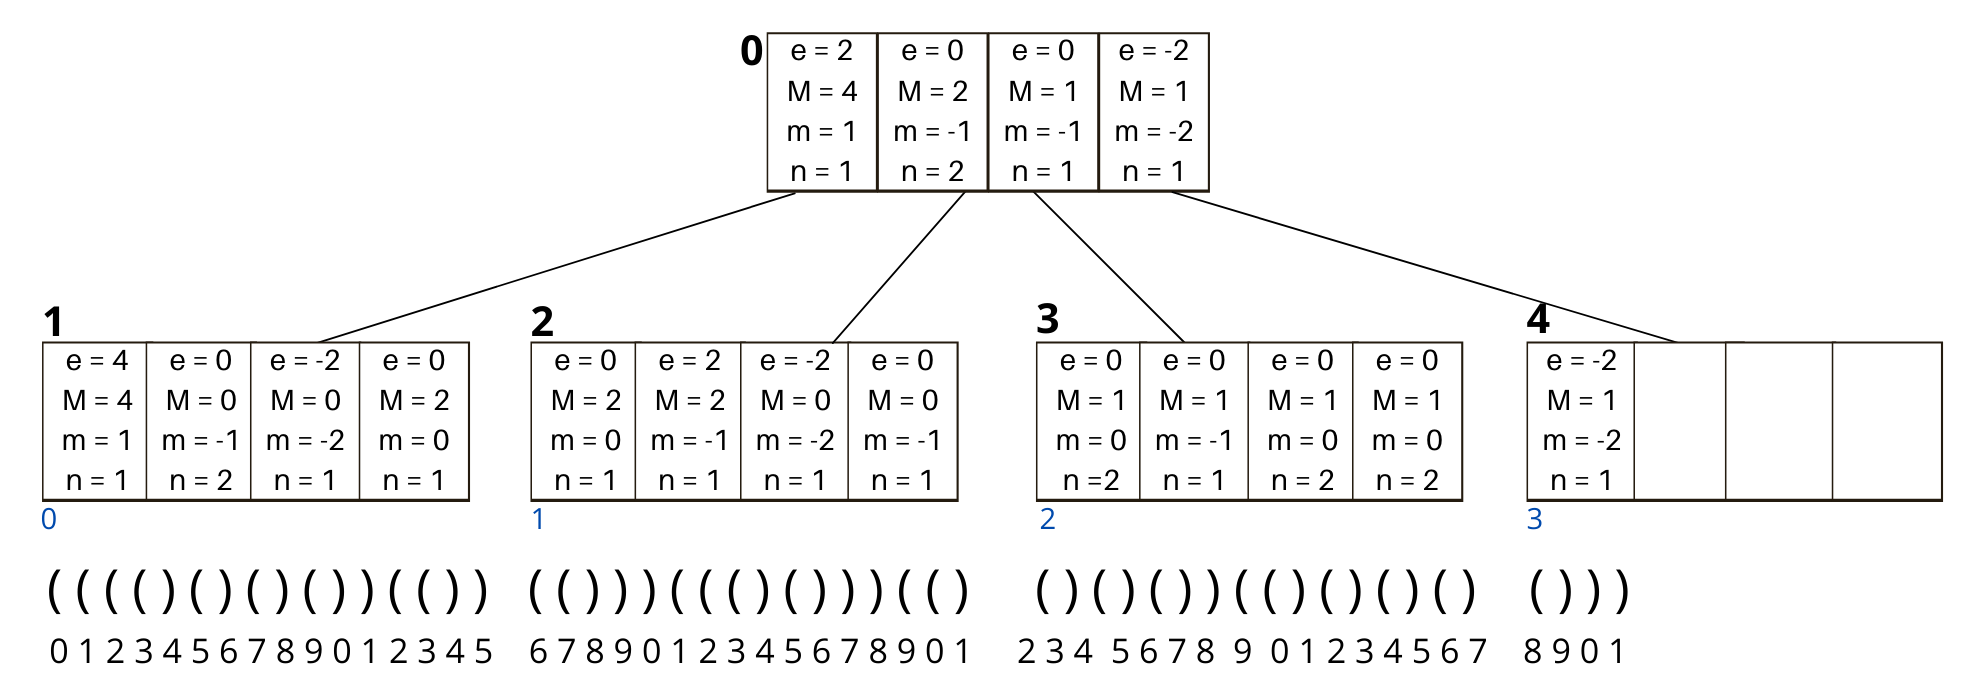
\includegraphics[width=\columnwidth]{images/rmm-tree-kary.png}
      \label{fig:rmm-tree-k}
    \end{figure}

    \begin{algorithm}[h!]
        \SetKwFunction{algo}{algo}
        \SetKwProg{myalg}{Algoritmo}{}{}
        \myalg{buildingTree(BP, C, k, b, w, r, nNodes)}{
    
            \Input{Vetor de bits, tabela de excessos C, aridade da árvore, tamanho de bloco e de subbloco, número de folhas e quantidade de nós.}
    
            \tcp{Construção dos nós folhas}
            $numReg \leftarrow 0$\tcp{Número de registros computados}
            \For{$l \leftarrow 0$ \textbf{to} $r -1$}{
                $v \leftarrow leafInTree(l)$\tcp{Análogo ao Algoritmo~\ref{alg:folha-indice}}
                $reg \leftarrow 0$\tcp{i-ésimo registro de um nó}
                \While{$R[v].nReg < k$ \textbf{and} $numReg < \ceil{BP.size()/b}$}{
                    $(R[v][reg], R[v][reg].M, R[v][reg].m, R[v][reg].n) \gets(0,-w,w,0)$\\
                    \For{$p \leftarrow (numReg\cdot (b/w))+1$ \textbf{to} $((numReg+1)\cdot b)/w$}{
                        $x \leftarrow bistread((p-1)\cdot w)$\\
                        \If{$R[v][reg].e + C[x].M > R[v][reg].M$}{$R[v][reg].M \leftarrow R[v][reg].e + C[x].M $}
                        \If{$R[v][reg].e + C[x].m < R[v][reg].m$}{
                        $R[v][reg].m \leftarrow R[v][reg].e + C[x].m $\\
                        $R[v][reg].n \leftarrow C[x].n$
                        }
                        \ElseIf{$R[v][reg].e + C[x].m = R[v][reg].m$}{$R[v][reg].n \leftarrow R[v][reg].n + C[x].n$}
                        $R[v][reg].e \leftarrow R[v][reg].e + C[x].e$
                    }
                    $R[v].nReg \leftarrow R[v].nReg  +1$\\
                    $numReg \leftarrow numReg +1$\\
                    $reg \leftarrow reg +1$
    
                } 
            }
            \tcp{Construção dos nós internos e raíz}
            \For{$v \leftarrow nNodes - r - 1 $ \textbf{to} $0$}{
                \For{$reg \leftarrow 0$ \textbf{to} $k-1$ \textbf{and} $(v\cdot k)+reg+1$ \textbf{to} $nNodes-1$}{
                    $child \leftarrow (k\cdot v)+1+reg$\tcp{j-ésimo filho de $v$}
                    $R[v][reg].e  \leftarrow R[child][0].e$\\
                    $R[v][reg].m \leftarrow R[child][0].m$\\
                    $R[v][reg].M \leftarrow R[child][0].M$\\
                    $R[v][reg].n \leftarrow R[child][0].n)$\\
    
    
                    \tcp{Pecorre cada registro de filho (\textit{child}) de $v$}
                    \For{$i \leftarrow 1$ \textbf{to} $R[child].nReg-1$}{
                        $R[v][reg].M = max(R[child][i-1].M,R[v][i-1].e + R[child][i].M) $\\
                        $R[v][reg].m = min(R[child][i-1].m,R[v][i-1].e + R[child][i].m) $\\
                        \If{$R[v][reg].m < R[child][i-1].e + R[child][i].m$}{
                            $R[v][reg].n \leftarrow R[child][i].n$
                        }
                        \ElseIf{$R[v][reg].m = R[child][i-1].e + R[child][i].m$}{
                            $R[v][reg].n \leftarrow R[v][reg].n  + R[child][i].n$
                        }
                        $R[v][reg].e \leftarrow R[child][i].e$\\
                    }
                }
    
            }
        } 
        \caption{Construção da range min-Max tree k-ária}
        \label{alg:build-kary-rmm-tree}
    \end{algorithm} 

O Algoritmo~\ref{alg:build-kary-rmm-tree} ilustra o processo de construção da rmM-tree k-ária. A tabela C, as funções \textit{bitsread, leafInTree} e \textit{numLeaf} -- algumas citadas nesse e em outros algoritmos -- seguem a mesma abordagem da rmM-tree clássica. O elemento \textit{nReg} associado à um nó $v$ corresponde, ao número de registros naquele nó.



\section{Operações}\label{sec:optimized-operation}
Para este trabalho a nossa estrutura fornece suporte às duas principais primitivas da Range min-Max tree clássica, fwdSearch e bwdSearch (além daquelas já suportadas pela estrutura de vetores de bits). Além destas duas, nossa árvore de intervalos máximos e mínimos, fornece suporte à 5 operações derivadas daquelas apoiadas pela estrutura de vetores de bits (sobre a qual a nossa árvore é construída), e outras 16 operações, que são derivadas das duas primitivas exploradas adiante.


\subsection{FwdSearch}\label{sec:fwdSearch}
Como já dito no capítulo anterior a operação foward search, realiza uma busca a partir de um índice \textit{i}, afim de encontrar a posição $j>i$, onde ocorre um excesso relativo \textit{d}.

Essa operação, nessa versão da rmM-tree, se dá parcialmente de igual forma ao do modo clássico: varremos primeiro o bloco da folha, em busca do excesso desejado, a partir de $i+1$.  A diferença é que agora precisamos verificar  até \textit{k} blocos de tamanho \textit{b} dentro de cada nó inspecionado na nossa estrutura. Para tanto, acrescentamos à fwdSearch em sua versão clássica duas outras funções, são elas fwdRegistry e fwdVerifySibling.

A primeira função é chamada sempre que estamos visitando um nó folha, ou seja no início da busca e ao final da mesma, quando já encontramos o nó alvo que contém a resposta.  A operação fwdRegistry tem por objetivo identificar o registro que contém o excesso buscado da folha analisada. O processo é muito similar à verificação de um nó na rmM-tree clássica: a cada registro pecorrido verificamos a asserção $dr + R[v][reg].m \leq d \leq dr + R[v][reg].M$, caso seja verdadeira, significa que encontramos o intervalo que contém a resposta desejada. Se a asserção for falsa, adicionamos ao excesso relativo computado até o momento ($dr$), o excesso local do registro que acabamos de visitar, seguindo para o próximo registro.  O Algoritmo \ref{alg:fwdRegistry} fornece mais detalhes de como esse processo de busca por excesso nas folhas funciona.

Caso o excesso buscado não seja encontrado na folha inicial, acionamos o processo de subida na árvore, aliado à nova função que mencionamos, \textit{fwdVerifySibling}. O objetivo dessa função é similar ao proposto por \citet{book-compact-data-structures}, quando o autor sugere que em cada nível verifiquemos se o excesso procurado está no irmão à direita do nó atual. Assim \textit{fwdVerifySibling} calcula a quantidade de irmãos do nó $v$ existentes à sua direita, e então analisa os registros de cada um deles em busca do intervalo que contém o excesso buscado, atualizando o valor de $dr$ sempre que $d$ não for encontrado em um registro.

Se ao final da inspeção dos irmãos de $v$, não encontrarmos o registro que contém a resposta, atualizamos o valor de $v$ para o índice do seu nó pai, e verificamos os irmãos deste nó atualizado. Repetimos esse processo até que seja encontrado um registro que contenha o excesso relativo desejado.

Tendo encontrado o intervalo que contém a resposta desejada durante a subida na rmM-tree, iniciamos  o processo de estreitamento desse intervalo, através do processo de descida na rmM-tree. Esta etapa é  similar as demais, e consiste em pecorrer os registros de um nó $v$, verificando se a asserção $dr + R[v][reg].m \leq d \leq dr + R[v][reg].M$ é válida, atualizando o valor do excesso computado até o momento, sempre que necessário. Ao inspecionarmos um registro que contém a resposta buscada,  atualizamos o valor de $v$, com base nesse registro, descendo mais um nível da árvore. Repetimos esse processo até que cheguemos à um nó folha, que é quando executamos novamente \textit{fwdRegistry}.

Os Algoritmos \ref{alg:fwdVerifySibling} e \ref{alg:fwdSearch} mostram como o processo de descida na árvore funciona, bem como o funcionamento completo de \textit{fwdSearch}.



O exemplo a seguir é baseado no Exemplo~\ref{ex:bin-fwdSearch} da Seção~\ref{sec:fwdsearch-bin}, e demonstra como podemos usar a operação \textit{fwdSearch} para obtermos a demarcação de término de um nó.
\begin{example}
Dado um nó em $BP$, codificado em $i=21$, encontrar o primeiro índice $j>i$, tal que $excess(j) - excess(i) = -1$.

O processo para a obtenção dessa resposta é descrito a seguir:

 O primeiro passo é identificar  o índice e o registro do nó folha que cobre $i=21+1$ (lembrando que a busca é por um $j > i$), neste caso temos $v = 2$ (folha $1$), e $reg = 1$, pois $\floor{(21 - 16)/4} = 1$. Assim iniciamos a varredura, pecorrendo o nó $v$, a partir de $i+1$ até o final do registro $1$. Ao finalizar a inspeção do registro que contém $i$, 
 temos que o excesso computado até o momento ($dr$) vale $2$, e portanto não encontramos o excesso buscado.
 
 \begin{figure}[h!]
    \centering
      \caption[fwdSearch(21,-1).]{Simulação da operação \textit{fwdSearch(21,-1)}.}
      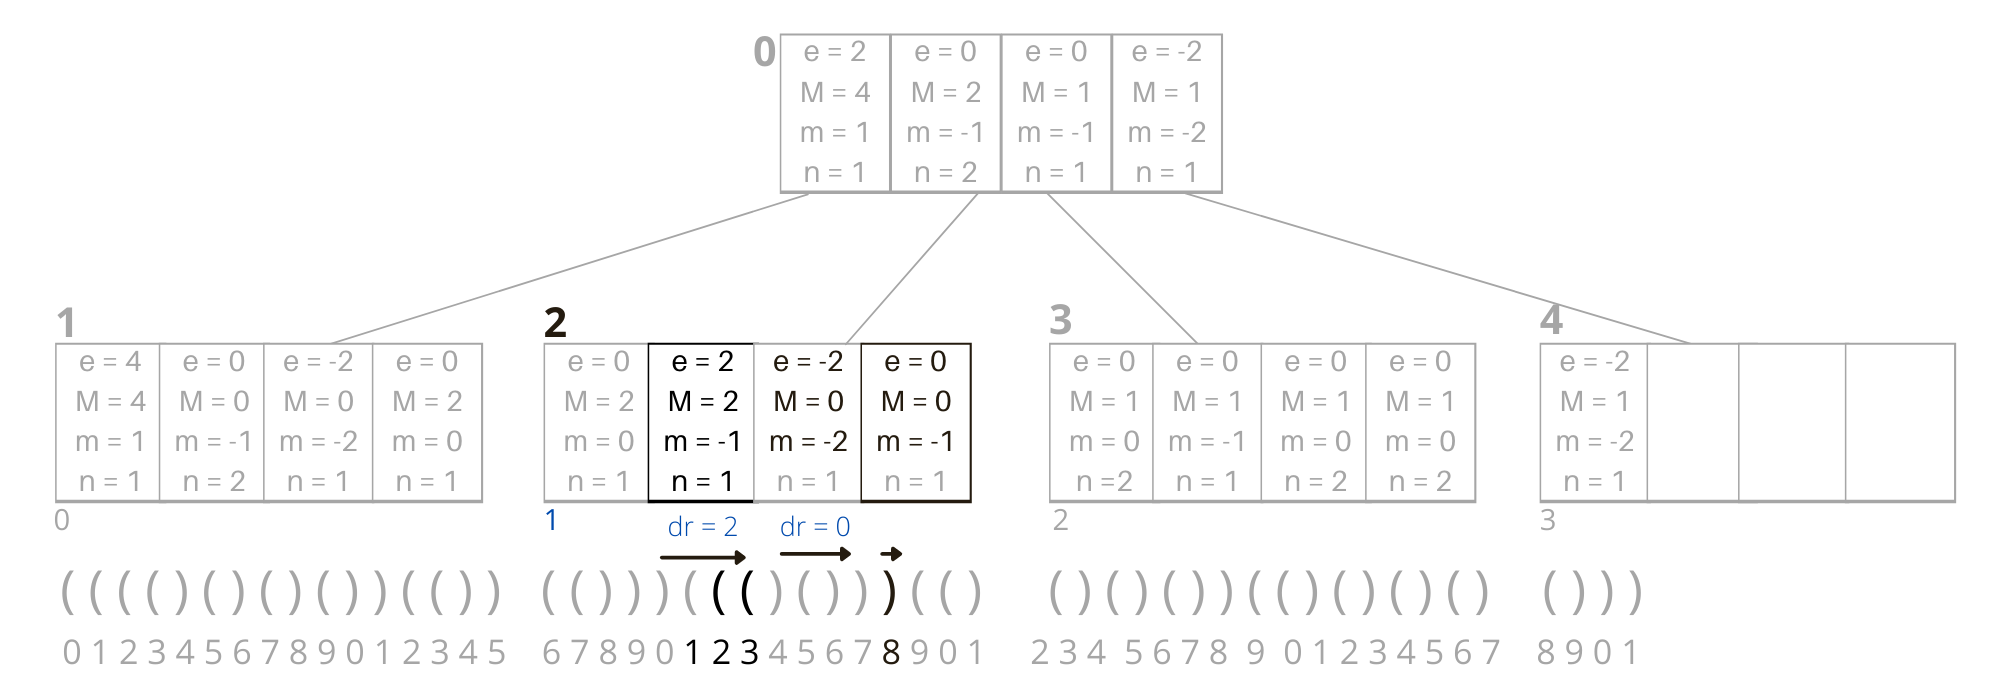
\includegraphics[width=\columnwidth]{images/rmm-tree-kary-fwdsearch.png}
      \label{fig:kary-fwdSearch}
 \end{figure}
\end{example}
Antes de verificarmos os irmãos do nó $v$, inspecionamos os registros restantes em $v$, analisando a cada momento se $dr + R[2][reg].m \leq d \leq dr + R[2][reg].M$. Ao verificar o registro $2$ do nó $v$, não encontramos o excesso buscado, atualizamos então o valor de $dr$, somando à ele $R[2][2].e$. Inspecionamos o último registro do nó $v=2$, e identificamos que $d$ está compreendido em seu intervalo. Interrompemos a análise dos nós da rmM-tree, e iniciamos uma análise mais detalhada da chave $3$, a fim de encontrar a posição exata onde $d$ ocorre. Durante essa inspeção, o valor de $dr$ atinge a marca $-1$, no índice $j=28$, encerrando assim a busca pelo excesso $d$ através de \textit{fwdSearch}.

 Perceba que neste exemplo foi necessário a inspeção de $2$ registros (excluindo o nó inicial), sem a necessida de realizar um percurso de subida na rmM-tree, ao passo que para o mesmo exemplo, na estrutura binária é necessário a inspeção de $5$ nós (excluindo o nó inicial), subir um nível, e depois descer um nível.

 \begin{algorithm}[htp]

    \SetKwFunction{algo}{algo}
    \SetKwProg{myalg}{Algoritmo}{}{}
    \myalg{fwdRegistry(i,v,reg,l,d,\&dr)}{
        \Input{Índice em $BP$, nó $v$, folha e registro correspondente, a partir dos quais a busca deve ser feita,  excesso relativo buscado, e excesso relativo computado em cada registro inspecionado ($d$ e $\&dr$). }
        \Output{Posição $j$ ou $BP.size()$ caso $d$ não seja encontrado.}
        \vspace{.3cm}
            \For{$reg$ \textbf{to}  $R[v].nReg -1$}{
                \If{$(dr + R[v][reg].m  \leq  d \leq  dr + R[v][reg].M)$}{
                    $j \leftarrow fwdBlock(i,d,dr)$\tcp{Algoritmo~\ref{alg:fwdBlock}}
                    \If{$dr = d$}{ \Return{$j$ }}

                }
                $dr \leftarrow dr +  R[v][reg].e$\\ 
                $i \leftarrow (k\cdot l+reg+1)\cdot b -1$ \tcp{calcula o fim da registro atual}
                \If{$dr = d$}{\Return{$i$ }}
            }
            \Return{$BP.size()$}
    }
    \caption{Busca pelo excesso $d$ entre os registros de uma folha.}
    \label{alg:fwdRegistry}
    \end{algorithm}
    
\begin{algorithm}[htp]
        \SetKwFunction{algo}{algo}
        \SetKwProg{myalg}{Algoritmo}{}{}
        \myalg{fwdVerifySibling(\&v,\&dr,d)}{
            \Input{Nó $v$,  excesso relativo buscado e excesso relativo computado até o momento e excesso buscado. }
            \Output{Registro $(reg)$ que contém a resposta, ou $BP.size()$ caso o intervalo que contém $d$ não seja encontrado.}
            \vspace{.3cm}
            $parent \leftarrow \floor{(v-1)/k}$ \\
            $n\_sibling \leftarrow v - (parent \cdot  k)$\\
            $v \leftarrow v + 1$\\
            \While{$n\_sibling$ \textbf{to}  $R[parent].nReg -1$ \textbf{and} $v$ \textbf{to} $num\_nodes - 1$}{
                \For{$reg \leftarrow 0$ \textbf{to} $R[v].nReg -1$}{
                    \If{($dr + R[v][reg].m  \leq  d \leq  dr + R[v][reg].M)$}{
                        \If{$v \leq numberNodes - numberLeaves$}{$v \leftarrow (v\cdot k)+1+reg$}
                        \Return{$reg$ }
                    }
                    $dr \leftarrow dr +  R[v][reg].e$\\
                    \If{$dr = d$}{
                        \If{$v \leq numberNodes - numberLeaves$}{$v \leftarrow (v\cdot k)+reg+2$}
                        \Return{$reg+1$ }
                    }
                }
                $n\_sibling \leftarrow n\_sibling + 1$\\
                $v \leftarrow v+1$\\
                %TODO preciso ser tão precisa?exibir todas as condições do meu código?Lembrando que estou trabalhando com referencia 
            }
            \Return{$BP.size()$ }
        }
        \caption{Analisa os registros dos írmãos de $v$ em busca do excesso $d$.}
        \label{alg:fwdVerifySibling}
    \end{algorithm}

\begin{algorithm}[htp]
    \SetKwFunction{algo}{algo}
    \SetKwProg{myalg}{Algoritmo}{}{}
    \myalg{fwdSearch(i,d)}{
        \Input{Índice a partir do qual a busca deve ser feita, excesso relativo buscado.}
        \Output{Posição $j$ onde ocorre o excesso $d$ ou $BP.size()$ caso $d$ não exista no intervalo definido.}
        \vspace{.3cm}
        $dr \leftarrow 0$\\
        $l \leftarrow \floor{(i+1)/(b\cdot k)}$\tcp{l-ésima folha}
        $v \leftarrow leafInTree(l)$\tcp{Número do registro inicial}
        $reg \leftarrow \floor{( (i+1) - (l\cdot b\cdot k))/b}$\\
        $j \leftarrow fwdBlock(i,d,dr)$\tcp{Algoritmo~\ref{alg:fwdBlock}}

        \If{$dr = d $}{\Return{$j$}}

        $reg \leftarrow reg +1$\\
        \If{$reg < R[v].nReg$}{
            $j \leftarrow fwdRegistry((k\cdot l+reg)\cdot b-1,v,reg,l,d,dr)$\\
            \lIf{$dr = d $}{\Return{$j$}}
        }
        \vspace{.3cm}
       \tcp{Inicia o processo de subida na rmM-tree}
        \While{$v \neq 0$ \textbf{and} $fwdVerifySibling(v,dr,d) = BP.size()$ }{
            $v \leftarrow \floor{(v-1)/m}$\\
        }
        
        \tcp{Chegamos ao nó raíz, e $d$ não está em nenhum dos seus filhos}
        \If{$v=0$ \textbf{and} $reg=v.size()$}{\Return{$v.size()$}}
        \vspace{.3cm}
        \tcp{Inicia descida em árvore}
        \While{$v \leq numberNodes - numberLeaves$}{
            \For{$reg \leftarrow 0$ \textbf{to} $R[v].nReg -1$}{
                \If{$(dr + R[v][reg].m  \leq  d \leq  dr + R[v][reg].M)$}{
                    $v \leftarrow (v\cdot k) + 1 + reg $\\
                    $reg \leftarrow 0 $\\
                    \textbf{break}
                }
                \lElse{
                    $dr \leftarrow dr +  R[v][reg].e$
                }

            }
        }
        $l \leftarrow numLeaf(v)$\\
        $i \leftarrow (k\cdot l\cdot chave)\cdot sizeBlock$  \tcp{Calcula o índice inicial da folha que queremos inspecionar}
        $j \leftarrow fwdRegistry(i-1,v,0,l,d,dr)$\\
        \lIf{$dr = d$}{ \Return{$j$}}
        \Return{$BP.size()$}
    }
    \caption{Busca pela posição $j>i$ onde ocorre o excesso relativo $d$.}
    \label{alg:fwdSearch}
    \end{algorithm}

\newpage
         
\subsection{BwdSearch}\label{sec:bwdSearch}
Como dito anteriormente, o processo para calcular bwdSearch é completamente análogo à fwdSearch, devendo termos cuidado apenas com as questões relacionadas à simetria dos dados abordadas no Capítulo~\ref{ch:fundamentacao}. Tendo isso em mente podemos construir uma função que verifica se o excesso buscado está entre os registros das folhas analisadas, assim como uma segunda função que inspeciona os registros dos $p$ irmãos de um nó $v$. Os Algoritmos \ref{alg:bwdRegistry}, \ref{alg:bwdVerifySibling} e \ref{alg:bwdSearch} mostram o pseudocódigo para as adaptações da estrutura k-ária.


Apenas para recapitularmos, temos as seguintes observações em relação à assimetria dos dados em  bwdSearch\footnote{Para mais detalhes, verifique a Seção~\ref{sc:bwdsearch}}:
\begin{itemize}
    \item A posição $i$ é incluída na contagem de excessos;
    \item Adicionamos $1$ ao excesso relativo computado a cada inspeção, quando passamos por um bit $0$, e subtraímos $1$ desse excesso quando varremos um bit codificado como $1$;
    \item $excess(i) + d $ é alcançado quando $dr - R[v][reg].e + R[v][reg].m \leq d \leq dr - R[v][reg].e + R[v][reg].M $ for verdadeiro.
\end{itemize}

O Exemplo~\ref{ex:kary-bwd}  demonstra como podemos realizar a busca por um parênteses de abertura que codifica um nó, dado o seu respectivo parênteses de fechamento, através da operação \textit{bwdSearch}. Este exemplo por sua vez, é equivalente ao Exemplo~\ref{ex:bin-bwd}.

\begin{example}\label{ex:kary-bwd}
    Dado um nó em $BP$, codificado em $i=50$, encontrar o  índice $j<i$ mais à direita de $i$,tal que $excess(j) - excess(i) = 0$.
    \begin{figure}[htp]
        \centering
          \caption[bwdSearch(50,0).]{Simulação da operação \textit{bwdSearch(50,0)}.}
          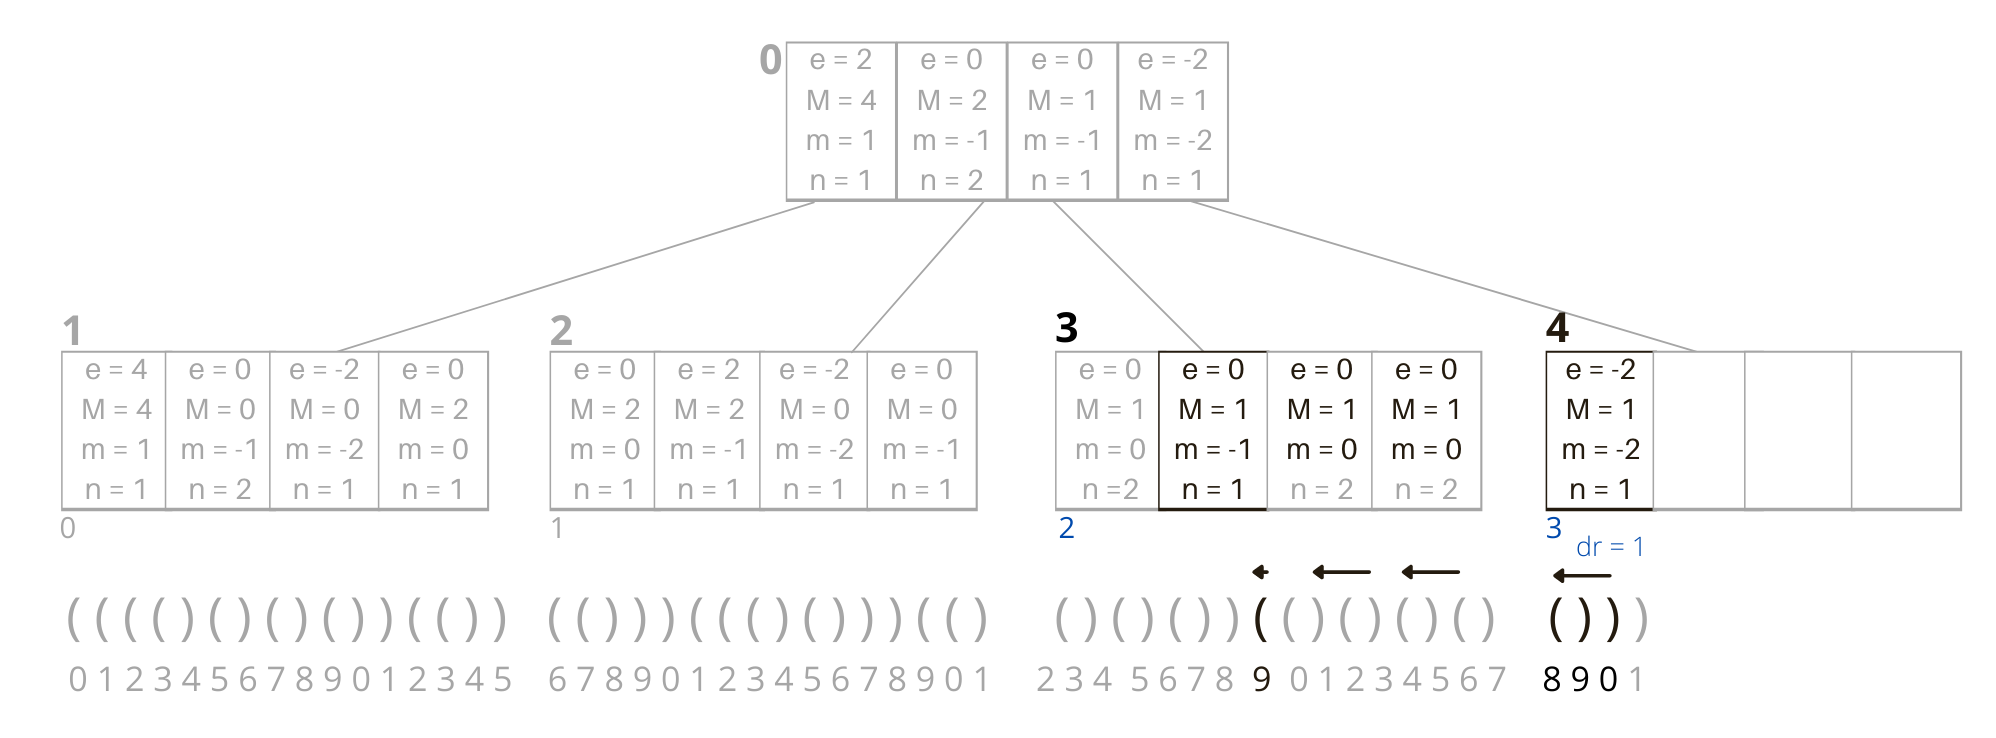
\includegraphics[width=\columnwidth]{images/rmm-tree-kary-bwdsearch.png}
          \label{fig:kary-bwdSearch}
     \end{figure}


     Após identificarmos o nó e o registro a qual pertence o índice $i=50$, temos que $v=4$ (folha $3$) e $reg = 0$ ($\floor{(50-48)/4}$). Iniciamos a inspeção da folha  $3$, partindo de  $i=50$, até alcançarmos o início da mesma que é $s=48$, ao término desta inspeção temos que $dr=1$. Como o nó $4$ não possui outros registros e a resposta não foi encontrada, realizamos a verificação dos registros localizados nos irmãos à esquerda do nó $v$.

     Atualizamos $v$ para o seu antecessor, que passa a valer $3$, pecorremos então cada um dos registros do nó $v=3$, verificando a asserção $dr - R[3][reg].e + R[3][reg].m \leq d \leq dr - R[3][reg].e + R[3][reg].M$. Inspecionamos os registros de número $3$ e $2$ do nó $v$ sem encontrar a resposta, ao analisarmos o registro $1$, temos que a asserção definida é verdadeira, neste momento encerramos a verificação dos nós da rmM-tree e iniciamos uma varredura mais detalhada deste registro. 

     Ao realizarmos a inspeção dos bits que compõe o registro $1$, do nó $3$, encontramos $dr=d$ em $j=49$, finalizando desse modo a busca pelo índice em $BV$ que codifica o parênteses de abertura correspondente à $i=50$;
     

     Para este exemplo fizemos a inspeção de $3$ registros (excluindo o registro inicial), já para a estrutura binária, como visto anteriormente, foi necessário, realizar a inspeção de  $6$ nós (excluindo o nó inicial), subir $1$ nível da árvore, descendo depois $2$ níveis.
     
    \end{example}

\begin{algorithm}[htp]
    \SetKwFunction{algo}{algo}
    \SetKwProg{myalg}{Algoritmo}{}{}
    \myalg{bwdRegistry(i,v,reg,l,d,\&dr)}{
        \Input{Índice em $BP$, nó $v$, folha e registro correspondente, a partir dos quais a busca deve ser feita,  excesso relativo buscado, e excesso  relativo computado em cada registro inspecionado ($d$ e $\&dr$). }
    \Output{Posição $j$ ou $-1$ caso $d$ não seja encontrado.}
    \vspace{.3cm}
    \For{$reg$ \textbf{downto}  $0$}{
        \If{$(dr - R[v][reg].e + R[v][reg].m \leq d \leq dr - R[v][reg].e + R[v][reg].M)$}{
            $j \leftarrow bwdBlock(i,d,\&dr)$\tcp{Análogo ao algoritmo~\ref{alg:fwdBlock}}
            \If{$dr = d$}{ \Return{$j$}}

        }
        $dr \leftarrow dr -  R[v][reg].e$\\ 
        $i \leftarrow (k\cdot l+reg)\cdot b-1$ \tcp{calcula o início da chave atual}
        \If{$dr = d$}{\Return{$i$ }}
    }
    \Return{$-1$ }
    }
\caption{Busca pelo excesso $d$ entre os registros de uma folha.}
\label{alg:bwdRegistry}
\end{algorithm}

\begin{algorithm}[htp]
    \SetKwFunction{algo}{algo}
    \SetKwProg{myalg}{Algoritmo}{}{}
    \myalg{bwdVerifySibling(\&v,\&dr,d)}{
    \Input{Nó $v$,  excesso relativo buscado e excesso relativo computado até o momento e excesso buscado. }
    \Output{Registro $(reg)$ que contém a resposta ou $-1$ caso o intervalo que contém $d$ não seja encontrado.}
    \vspace{.3cm}
    $parent \leftarrow \floor{(v-1)/k}$ \\
    $n\_sibling \leftarrow v - (parent \cdot k) -1 $\\
    $v \leftarrow v - 1$\\
    \While{$n\_sibling$ \textbf{downto}  $0$ \textbf{and} $v$ \textbf{downto} $0$}{
        \For{$reg \leftarrow R[v].nReg -1$ \textbf{to} $0$}{
            \If{$(dr - R[v][reg].e + R[v][reg].m \leq d)$ \textbf{and} $(d \leq dr - R[v][reg].e + R[v][reg].M)$}{
                lIf{$v \leq numberNodes - numberLeaves$}{$v \leftarrow (v\cdot k)+1+reg$}
                \Return{$reg$ }
            }
            $dr \leftarrow dr -  R[v][reg].e$\\
            \If{$dr = d$}{
                \If{$v \leq numberNodes - numberLeaves$}{$v \leftarrow (v\cdot k)+reg$}
                \Return{$reg$ }
            }
        }
        \If{$n\_sibling -1 > 0$}{$v \leftarrow v-1$}
        $n\_sibling \leftarrow n\_sibling - 1$\\
    }
    \Return{$-1$}
    }
    \caption{Analisa os registros dos írmãos de $v$ em busca do excesso $d$.}
    \label{alg:bwdVerifySibling}
\end{algorithm}

\begin{algorithm}[htp]
    \SetKwFunction{algo}{algo}
    \SetKwProg{myalg}{Algoritmo}{}{}
    \myalg{bwdSearch(i,d)}{
    \Input{Índice a partir do qual a busca deve ser feita, excesso relativo buscado.}
    \Output{Posição $j$ onde ocorre o excesso $d$ ou $-1$ caso $d$ não exista no intervalo definido.}
    \vspace{.3cm}
        $dr \leftarrow 0$\\
        $l \leftarrow \floor{i/(b\cdot k)}$\tcp{l-ésima folha}
        $v \leftarrow leafInTree(l)$\\
        $reg \leftarrow \floor{((i+1) - (l\cdot b\cdot k))/b}$\tcp{Número do registro inicial}
        $j \leftarrow bwdBlock(i,d,\&dr)$\tcp{Análogo ao algoritmo~\ref{alg:fwdBlock}}
        \If{$dr = d $}{\Return{$j$}}

        $reg \leftarrow reg -1$\\
        \If{$reg \geq 0$}{
            $j \leftarrow bwdRegistry((k\cdot l+reg+1)\cdot b-1,v,reg,l,d,\&dr)$\\
            \If{$dr = d $}{\Return{$j$}}

        }
        \vspace{.3cm}
        \tcp{Inicia o processo de subida na rmM-tree}
        \While{$v \neq 0$ \textbf{and} $bwdVerifySibling(\&v,\&dr,d) = -1$ }{
            $v \leftarrow \floor{(v-1)/k}$\\
        }
        \tcp{Chegamos ao nó raíz,  mas $d$ não está em nenhum dos seus filhos}
        \If{$v=0$ \textbf{and} $reg=-1$}{\Return{$-1$}}
        \vspace{.3cm}
        \tcp{Desce nível a nível da árvore, até que $v$ corresponda ao índice de um dos nós folhas}
        \While{$v \leq numberNodes - numberLeaves$}{
            \For{$reg \leftarrow R[v].nReg - 1$ \textbf{to} $0$}{
                \If{$(dr - R[v][reg].e +R[v][reg].m \leq d \leq dr - R[v][reg].e +R[v][reg].M)$}{
                    $v \leftarrow (v\cdot k) + 1 + reg $\\
                    $reg \leftarrow R[v].nReg-1 $\\
                    \textbf{break}
                }
                \Else{
                    $dr \leftarrow dr - R[v][reg].e$
                }

            }
        }
        \vspace{.3cm}
        $l \leftarrow numLeaf(v)$\\
        \If{$d = dr$}{\Return{$(l\cdot k\cdot b) + (reg\cdot b)-1$}}
        $j \leftarrow bwdRegistry((l\cdot k\cdot b)+((reg+1)\cdot b)-1, v,reg,l,d,\&dr)$\\
        \lIf{$dr = d$}{ \Return{$j$}}
        \lElse{
            \Return{$-1$}
        }
    }
    \caption{Busca pela posição $j>i$ onde ocorre o excesso relativo $d$.}
    \label{alg:bwdSearch}
    \end{algorithm}

\newpage
     \subsection{Derivadas}
     Não entraremos nos detalhes das operações derivadas de \textit{fwdSearch} e \textit{bwdSearch}, tendo em vista que as mesmas já foram explanadas no Capítulo~\ref{ch:fundamentacao}.  
     
     A Tabela~\ref{tbl:karyOperations-rmm-tree} traz um comparativo das operações suportadas pela rmM-tree k-ária e binária. Para a rmM-tree k-ária oferecemos suporte à um número menor de operações. Isso se deve ao fato de que não implementamos as operações de \textit{minExcess, maxExcess, minCount} e \textit{minSelectExcess} que são base de muitas outras, destaca-se porém, que o processo de adaptação destas operações é similar ao que já foi exposto até aqui.

     \begin{table}[h!]
	\centering
	\caption[Operações sobre a rmM-tree binária e k-ária]{Operações suportadas pela rmM-tree binária e rmM-tree-kária}
	\label{tbl:karyOperations-rmm-tree}
	\rowcolors{2}{lightgray!30}{white}
	\resizebox{\columnwidth}{!}{
	\begin{tabular}{lll}
	\toprule
	\textbf{Operação} & \textbf{rmM-tree binária} & \textbf{rmM-tree k-ária}\\
	\toprule
    
	fwdSearch(i,d)  &  \cmark \par &   \cmark \par\\
	bwdSearch(i,d)  &  \cmark \par &   \cmark \par\\
	minExcess(i,j) / maxExcess(i,j)  &   \cmark \par & \xmark \\
	minCount(i,j)  &   \cmark \par & \xmark\\
	minSelectExcess(i,j,t)  &  \cmark \par & \xmark\\
	enclose(i) &  \cmark \par &   \cmark \par \\
	rmq(i,j) / rMq(i,j) &  \cmark \par & \xmark \\
	rank$_1$(i) / rank$_0$(i) &  \cmark \par &    \cmark \par\\
    select$_1$(i) / select$_0$(i) &  \cmark \par &   \cmark \par\\
    preRank(i)/postRank(i) &  \cmark \par &   \cmark \par\\
    preSelect(i)/postSelect(i) &  \cmark \par &   \cmark \par \\
    isLeaf(i) &  \cmark \par &   \cmark \par\\
    isAncestor(i,j) &  \cmark \par &   \cmark \par\\
    depth(i) &   \cmark \par &   \cmark \par\\
    parent(i) &  \cmark \par &   \cmark \par\\
    firstChild(i) / lastChild(i) &  \cmark \par &   \cmark \par\\
    child(i,t)&  \cmark \par & \xmark \\
    nextSibling(i) / prevSibling(i) &   \cmark \par &   \cmark \par\\
    subtreeSize(i) &   \cmark \par &   \cmark \par\\
    levelAncestor(i,d) &   \cmark \par &   \cmark \par \\
    levelNext(i) / levelPrev(i) &   \cmark \par &   \cmark \par \\
    levelLeftMost(d) / levelRightMost(d) &  \cmark \par &   \cmark \par\\
    lca(i,j)&  \cmark \par & \xmark\\
    deepestNode(i)&  \cmark \par & \xmark \\
    degree(i)&  \cmark \par & \xmark\\
    childRank(i)&  \cmark \par & \xmark\\
    leafRank(i)&  \cmark \par &   \cmark \par\\
    leafSelect(i)&  \cmark \par  &   \cmark \par\\
    leftMostLeaf(i)&   \cmark \par &   \cmark \par\\
    rightMostLeaf(i)&   \cmark \par &   \cmark \par\\
	\bottomrule
	\end{tabular}
	}
\end{table}

  \chapter{Resultados Experimentais}\label{chp:resultados}

Este capítulo discorre sobre os procedimentos realizados para a obtenção dos resultados comparativos da rmM-tree proposta por \citet{paper-fully-functinal-succint-trees},
com a rmM-tree k-ária proposta neste trabalho. Ele está dividido da seguinte forma: a Seção ~\ref{sec:base-de-dados} apresenta o conjunto de dados usado na avaliação experimental.
As seções seguintes apresentam as configurações da máquina usada para realizar os testes (Seção~\ref{sec:configuracao}), a metodologia usada (Seção~\ref{sec:experimentos}), e por último os resultados obtidos (Seção~\ref{sec:resultados}).


\section{Base de dados}\label{sec:base-de-dados}
Afim de realizar testes que comprovem o desempenho das estruturas implementadas na prática, usamos em nossos testes quatro conjuntos de dados do mundo real, estes conjuntos são apresentados em \citet{datasets-inf-udec}.
A Tabela~\ref{tbl:dataset} mostra um resumo dos conjuntos usados: a primeira coluna da tabela refere-se ao nome do conjunto de dados, a segunda coluna indica o tamanho do conjunto de dados em MB, a coluna de número 3 mostra a quantidade de parênteses do respectivo conjunto de dados, e por fim, a quarta coluna exibe a quantidade de nós da árvore representada pela sequência de parênteses balanceados.


\begin{table}[h!]
  \centering
  \caption[Conjunto de dados usados em testes experimetais]{Conjunto de dados usados nos testes experimetais }
  \label{tbl:dataset}
	\resizebox{\columnwidth}{!}{
        \begin{tabular}{|l|l|l|l|l|}
        \hline
        \textbf{Conjunto de dados}                       & \textbf{Tamanho (MB)}                      & \textbf{Quantidade de parênteses}                      & \textbf{Tamanho da árvore representada}  \\ \hline
        Complete tree (ctree)                            & 18                                          & 2.147.483.644                                          & 1.073.741.822                           \\ \hline
        DNA                                              & 135                                         & 1.154.482.174                                          & 577.241.087                             \\ \hline
        Proteins (prot)                                  & 82                                          & 670.721.006                                            & 335.36203                               \\ \hline
        Wikipedia   (wiki)                               & 13                                          & 498.753.914                                            & 249.376.957                             \\ \hline
        \end{tabular}
    }
\end{table}

Conforme é mostrado em \citet{datasets-inf-udec}, o  conjunto \textit{Complete tree} represeta uma árvore binária completa de profundidade igual à 30, ao passo que as sequências  de parênteses balanceados $DNA$/$Proteins$ representam uma árvore de sufixos de DNA e proteínas, respectivamente. Por último o conjunto \textit{Wikipedia} representa o XML extraído da Wikipédia no dia 12 de janeiro de 2015 \citep{datasets-inf-udec}.

\section{Configuração}\label{sec:configuracao}
Para realizar os testes de validação e de comparação de desempenho foi utilizado o servidor Turing, disponível no IFB. A máquina usada possui as seguintes configurações:
\begin{itemize}
    \item Arquitetura: x86;
    \item Processador: Intel Xeon Gold 5120;
    \item Frequência base: 2,20GHz;
    \item Frequência máxima: 3,20 GHz;
    \item Threads por core: 2;
    \item Cores: 28;
    \item Cache L1: 896 KiB;
    \item Cache L2: 28 MiB;
    \item Cache L3: 38.5 MiB, e
    \item Memória RAM total: 527,03 Gb.
\end{itemize}

\section{Experimentos}\label{sec:experimentos}
\subsection{Decisões de projeto}\label{subsec:decision}
Os conjuntos mostrados acima fornecem árvores no formato de parênteses balanceados, de modo que foi preciso pré-processar os conjuntos antes da execução dos testes, afim de transformar parênteses de abertura e de fechamento em bits $1's$ e $0's$, respectivamente.

Para realizarmos uma comparação justa entre a estrutura proposta por \citet{paper-fully-functinal-succint-trees} e a estrutura proposta neste trabalho,  implementamos a rmM-tree no seu formato binário seguindo a descrição de \citet{book-compact-data-structures}. Após a implementação e validação dessa estrutura em seu formato binário, iniciamos a construção e validação da rmM-tree k-ária. Ambas as estruturas estão disponíveis no repositório \href{https://github.com/DanyelleAngelo/rmm-tree}{github.com/DanyelleAngelo/rmm-tree}, usando a linguagem de programação \textit{C++} e a biblioteca \textit{SDSL} \citep{sdsl-article}. 

Durante os testes de desempenho (descritos com mais detalhes na Seção ~\ref{sec:benchmark}), fizemos algumas adaptações na nossa proposta, assim implementamos duas versões da rmM-tree k-ária, estas se diferem unicamente pelo processo de subida na árvore. A primeira versão (adotada neste trabalho), segue a abordagem de verificação dos irmãos à direita  (ou à esquerda, dependendo do sentido da busca) de um nó $v$, durante o percurso em árvore, como descrito por \citet{book-compact-data-structures}, para esta versão, o pior caso é observado durante uma busca iniciada em um nó $v$, com o excesso desejado não estando compreendido entre os registros dos irmãos de $v$, e $v$ sendo um dos primeiros filhos de seu nó pai. Buscando evitar este caso, construímos uma versão alternativa da rmM-tree k-ária, que não faz uso da técnica de visitação dos nós vizinhos proposta por \citet{book-compact-data-structures}, nesta versão ao terminarmos de inspecionar os registros de um nó $v$, avançamos na rmM-tree através do seu nó pai, verificando os registros deste nó, e inspecionando os demais filhos deste, apenas se a resposta estiver compreendida entre os seus registros.   

Outra importante decisão no projeto das nossas estruturas e que melhorou significativamente o seu desempenho, foi a implementação da função \textit{bitsread} como é exposto na Seção ~\ref{sec:sec-classic-rmm-tree}. Inicialmente essa função lia de modo iterativo $w-1$ bits a partir de um índice $i$, e realizava então uma pesquisa na tabela \textit{C} pelo elemento correspondente aos bits lidos, obtendo assim os valores de excesso necessários para a computação de diversas operações. Essa leitura iterativa acrescentava um tempo considerável às nossas operações. Substituímos então esse processo iterativo, por um processo usando operações de deslocamento de bits, inserimos também em nosso projeto, o uso de uma tabela de reversão, para que pudessemos realizar a leitura dos bits, usando como critério de ínicio, o bit mais significativo da palavra.

\subsection{Testes unitários}
Objetivando garantir a asserção das respostas retornadas pela estrutura da rmM-tree binária e k-ária, realizamos a cada implementação -- e alteração  -- testes unitários usando o framework Google Tests.

No ínicio do desenvolvimento de cada estrutura foram criados testes com árvores gerais pequenas, comparamos os resultados da nossa implementação da rmM-tree binária, com os resultados da rmM-tree implementada na biblioteca \textit{Succint Data Structure Library} (SDSL), disponiblizada por \citet{sdsl-article}. Para algumas operações foi necessário computar o valor de retorno esperado usando uma série de operações básicas de vetores de bits, tendo em vista  que a SDSL não fornecia todas as operações necessárias para os testes de validação da nossa estrutura.

Após os primeiros testes de unidade, expandimos o nosso escopo de testes. Utilizando a sequência de parênteses \textit{Wikipedia}, geramos diversas consultas aleatórias afim de testar as operações da estrutura k-ária frente a estrutura binária.

No caso das operações que requeriam que o parâmetro de entrada correspondesse à um parênteses de abertura "(" ou de fechamento ")", foram pré-processados de modo aleatório os índices que atendiam a especificação, afim de realizarmos testes com entradas válidas.

\subsection{Testes de Desempenho}\label{sec:benchmark}
Após a construção de cada estrutura e tendo concluído os testes de validação, iniciamos os testes de desempenho, para tanto foi usado o framework Google Benchmark. Durante esses testes, foram introduzidas as melhorias citadas na Seção~\ref{subsec:decision}, sendo que à cada nova alteração, realizavamos novamente, todos os testes unitários, e testes de desempenho, afim de garantir a asserção dos nossos resultados.

Para os testes de desempenho, foram pré-computados diversos vetores pseudo-aleatórios, usando diferentes sementes (afim de manter uma variedade maior dos parâmetros usados), para diferentes operações. Cada um desses vetores tinham como entrada  índices dos conjuntos de dados usados nos testes, que caracterizam parâmetros válidos para as operações sobre as rmM-tree implementadas. 

Para cada operação foi usado cerca de $3.000.000$ de dados, os resultados de desempenho das mesmas é mostrado na próxima seção.

\section{Resultados}\label{sec:resultados}
O tempo gasto por cada operação da rmM-tree binária e k-ária sobre os conjuntos de dados citados, foi exportado para um arquivo \textit{.csv}, e a partir destes resultados, foram gerados gráficos de tempo médio gasto por cada operação, através da linguagem de programação Python. Estes gráficos são mostrados nas Figuras~\ref{fig:cstree}, \ref{fig:dna}, \ref{fig:prot} e \figref{fig:wiki}.

Os gráficos de barras aninhadas, agrupam os resultados para cada tipo de árvore por operação. As árvores geradas para os testes são:
\begin{itemize}
  \item rmM-tree binária (barra azul);
  \item rmM-tree 4-ária (barra laranja);
  \item rmM-tree 8-ária (barra verde), e
  \item rmM-tree 16-ária (barra vermelha).
\end{itemize}

 O tamanho de bloco usado em todos os testes foi definido como $32$, e a constante $w$ que divide $b$, foi setada como $16$, mantendo assim a tabela C, que auxilia na montagem da árvore e na verificação dos dados em cache.

O eixo $y$ dos nossos gráficos se refere ao tempo médio para $3.000.000$ consultas sobre as diferentes versões da rmM-tree, no eixo $x$ podemos ver os tipos de árvores comparadas, bem como as operações realizadas. 

Ressalta-se novamente que as operações \textit{minExcess, minSelectExcess, minCount} e suas derivadas não foram implementadas na nossa versão k-ária da rmM-tree, e por isso o desempenho das mesmas não foram levados em consideração pela nossa análise, além destas também não realizamos testes de benchmark para as operações que derivam exclusivamente de operações de acesso ao vetor que representa a árvore de entrada.

Como pode ser observado nos gráficos, a rmM-tree binária obteve melhor desempenho para todas as operações, isso está relacionado ao fato de que a rmM-tree binária, possui uma série de otimizações a nível de código, que não são implementadas na rmM-tree k-ária. Por exemplo, para a rmM-tree binária, o percurso em árvore é interrompido sempre que atingimos o último nó de um nível (ou primeiro de um nível, para o caso da operação \textit{bwdSearch}), o que não acontece na rmM-tree k-ária.

Além disso, o hardware utilizado possui uma cache relativamente grande em comparação aos conjuntos de dados analisados, desta forma os dados tendem a residir sempre em cache, inviabilizando a análise comparativa dos resultados encontrados pela rmM-tree binária e k-ária, haja vista que esta última deveria apresentar melhor resultado quando obtém uso otimizado da cache frente a estrutura original. 

Para as aridades da rmM-tree k-ária analisadas, não foi possível detectar um padrão para os diferentes conjuntos de dados. No geral, o desempenho das estruturas \textit{k-árias} variam entre si, para cada operação em unidades de \textit{nanossegundos}. Novamente isso se deve ao tamanho da cache utilizada, como afirmado anteriormente, com os dados residindo sempre em cache, torna-se desprezível as diferentes aridades de árvores. 

Com base no conteúdo abordado neste trabalho, acredita-se que mediante à implementação de otimizações no código da rmM-tree k-ária, poderemos atingir o equilíbrio entre a quantidade de instruções executadas, e acessos a memória principal, melhorando assim o desempenho do sistema. Acredita-se também que a estrutura proposta mostrará seu potencial diante de um hardware mais modesto.

\newpage

\begin{figure}[!ht]
    \centering
      \caption[Operações sobre o conjunto de dado ctree]{Tempo médio de operações sobre o conjunto Complete Tree}{
          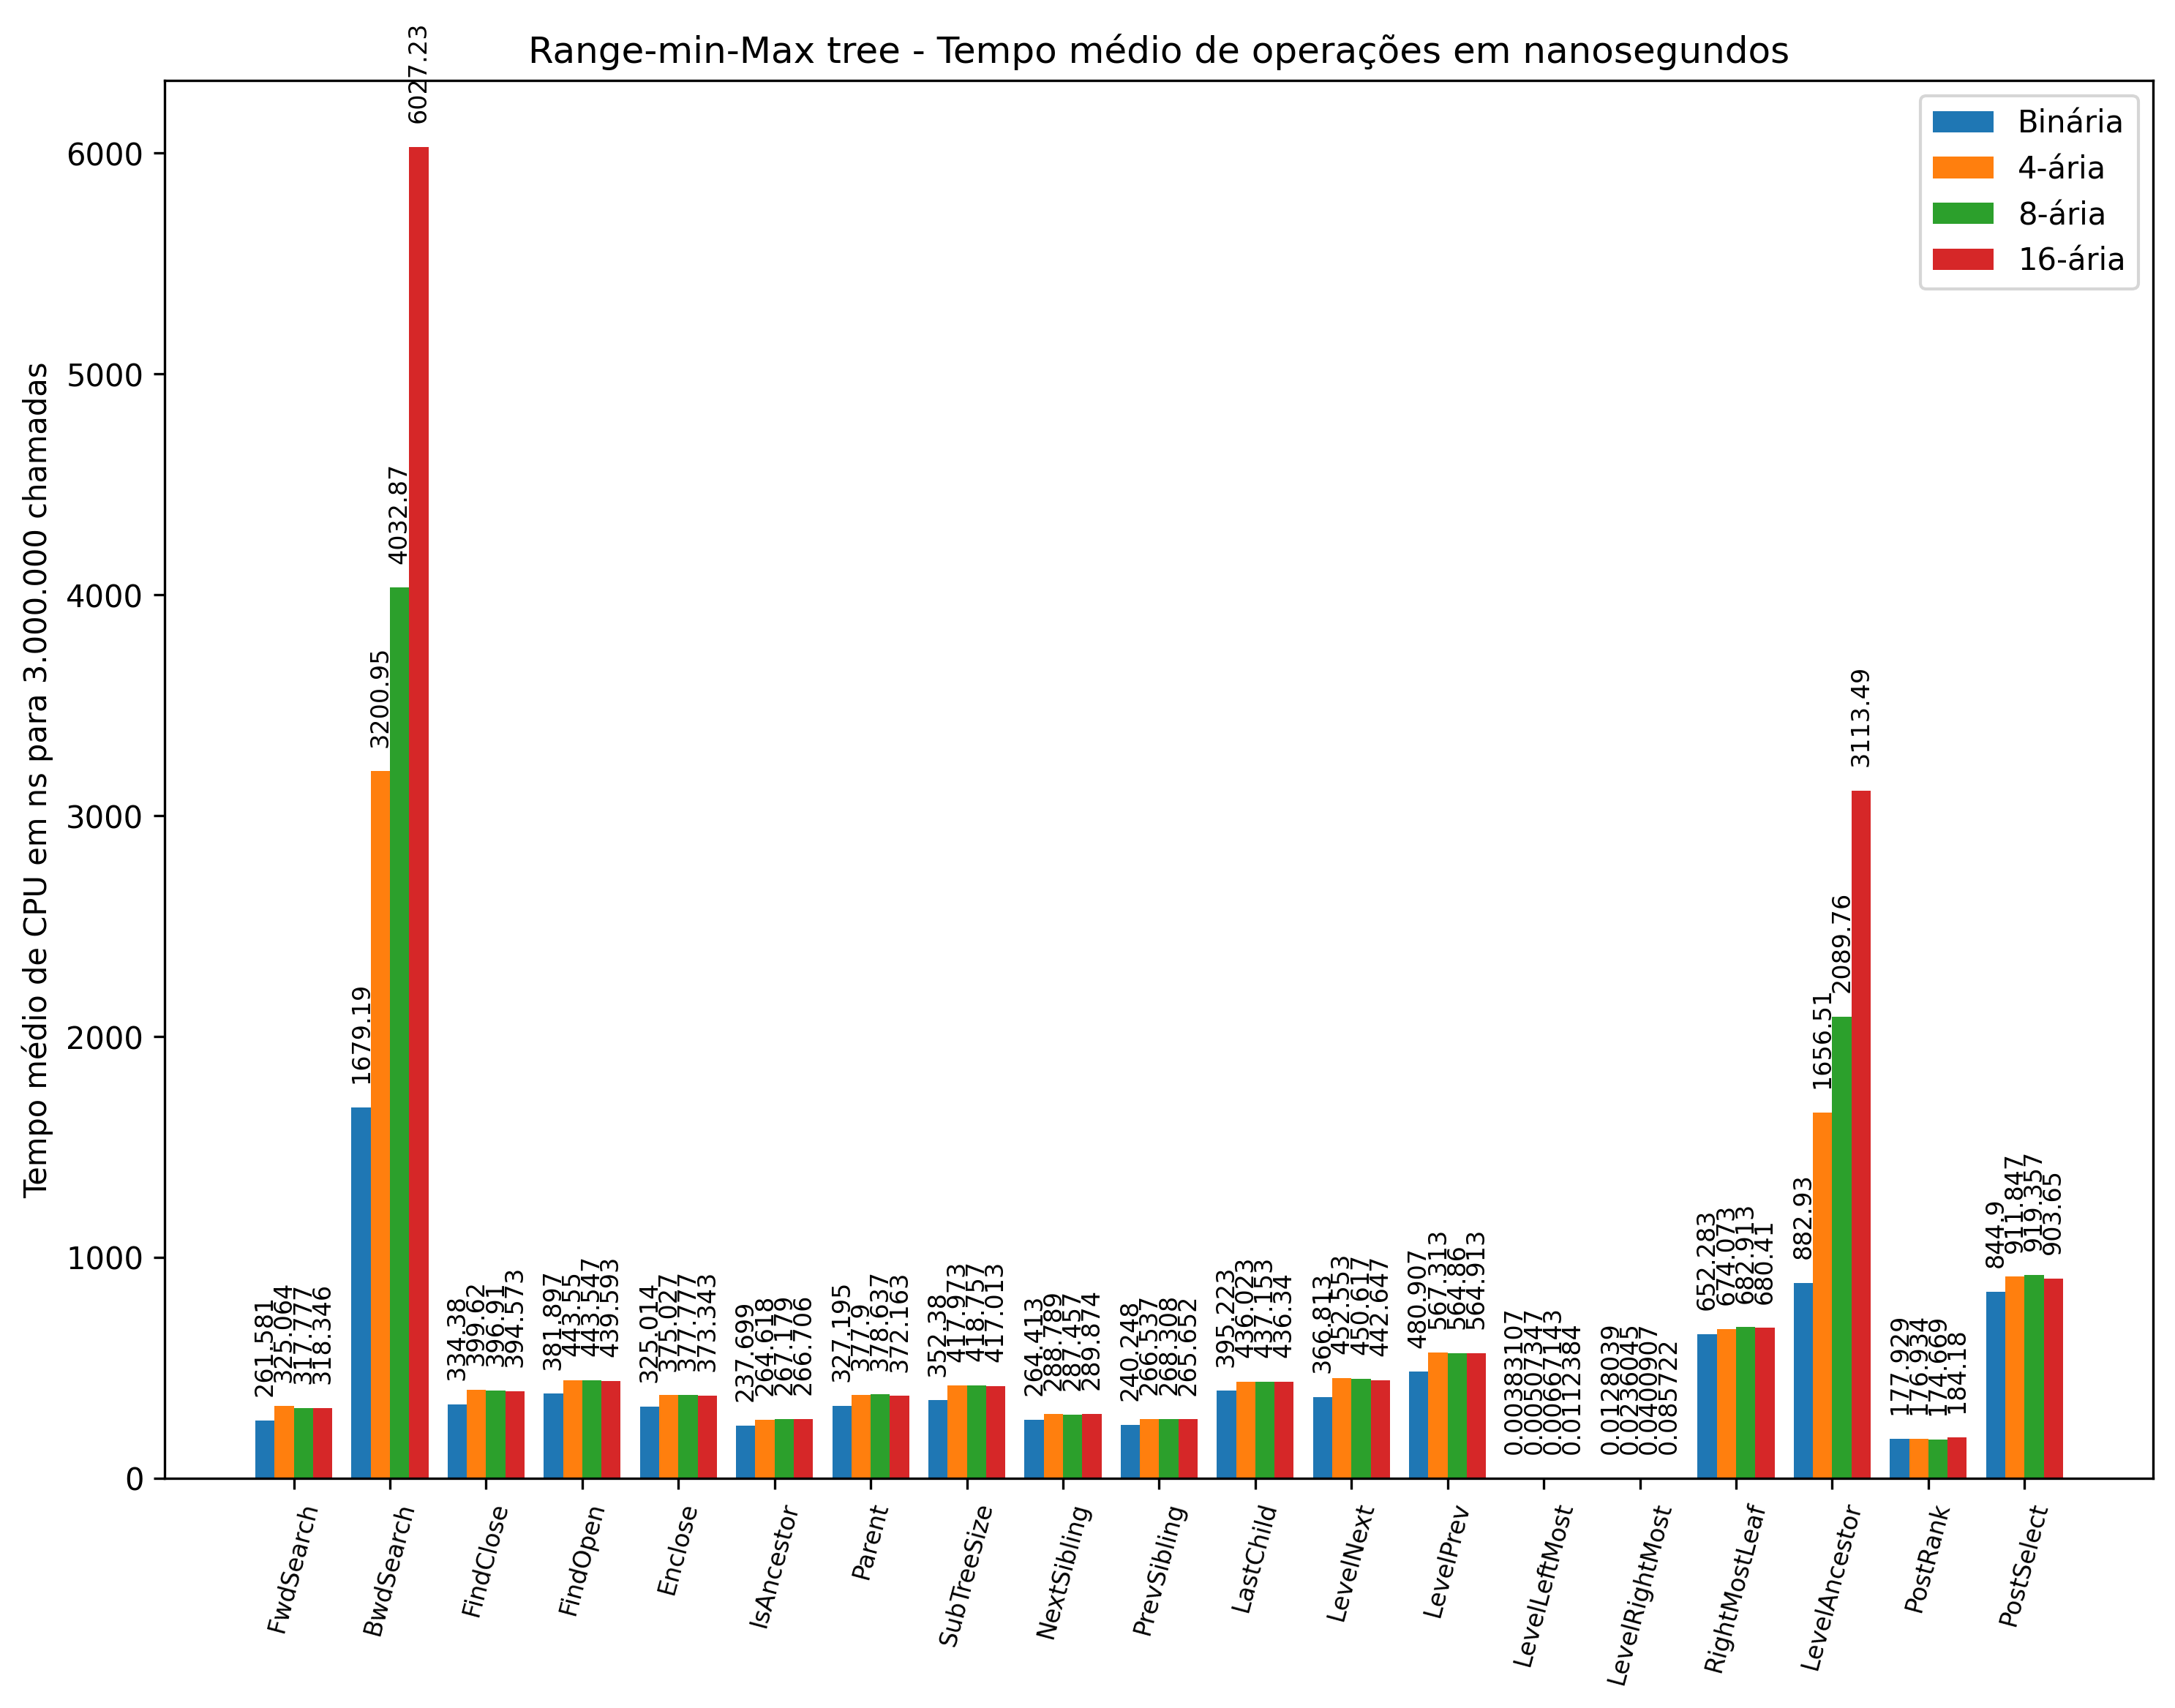
\includegraphics[scale=0.8, angle=270]{images/ctree_i3000000.png}
        }
        \label{fig:cstree}
\end{figure}

\begin{figure}[!ht]
    \centering
      \caption[Operações sobre o conjunto de dado dna]{Tempo médio de operações sobre o conjunto DNA}{
          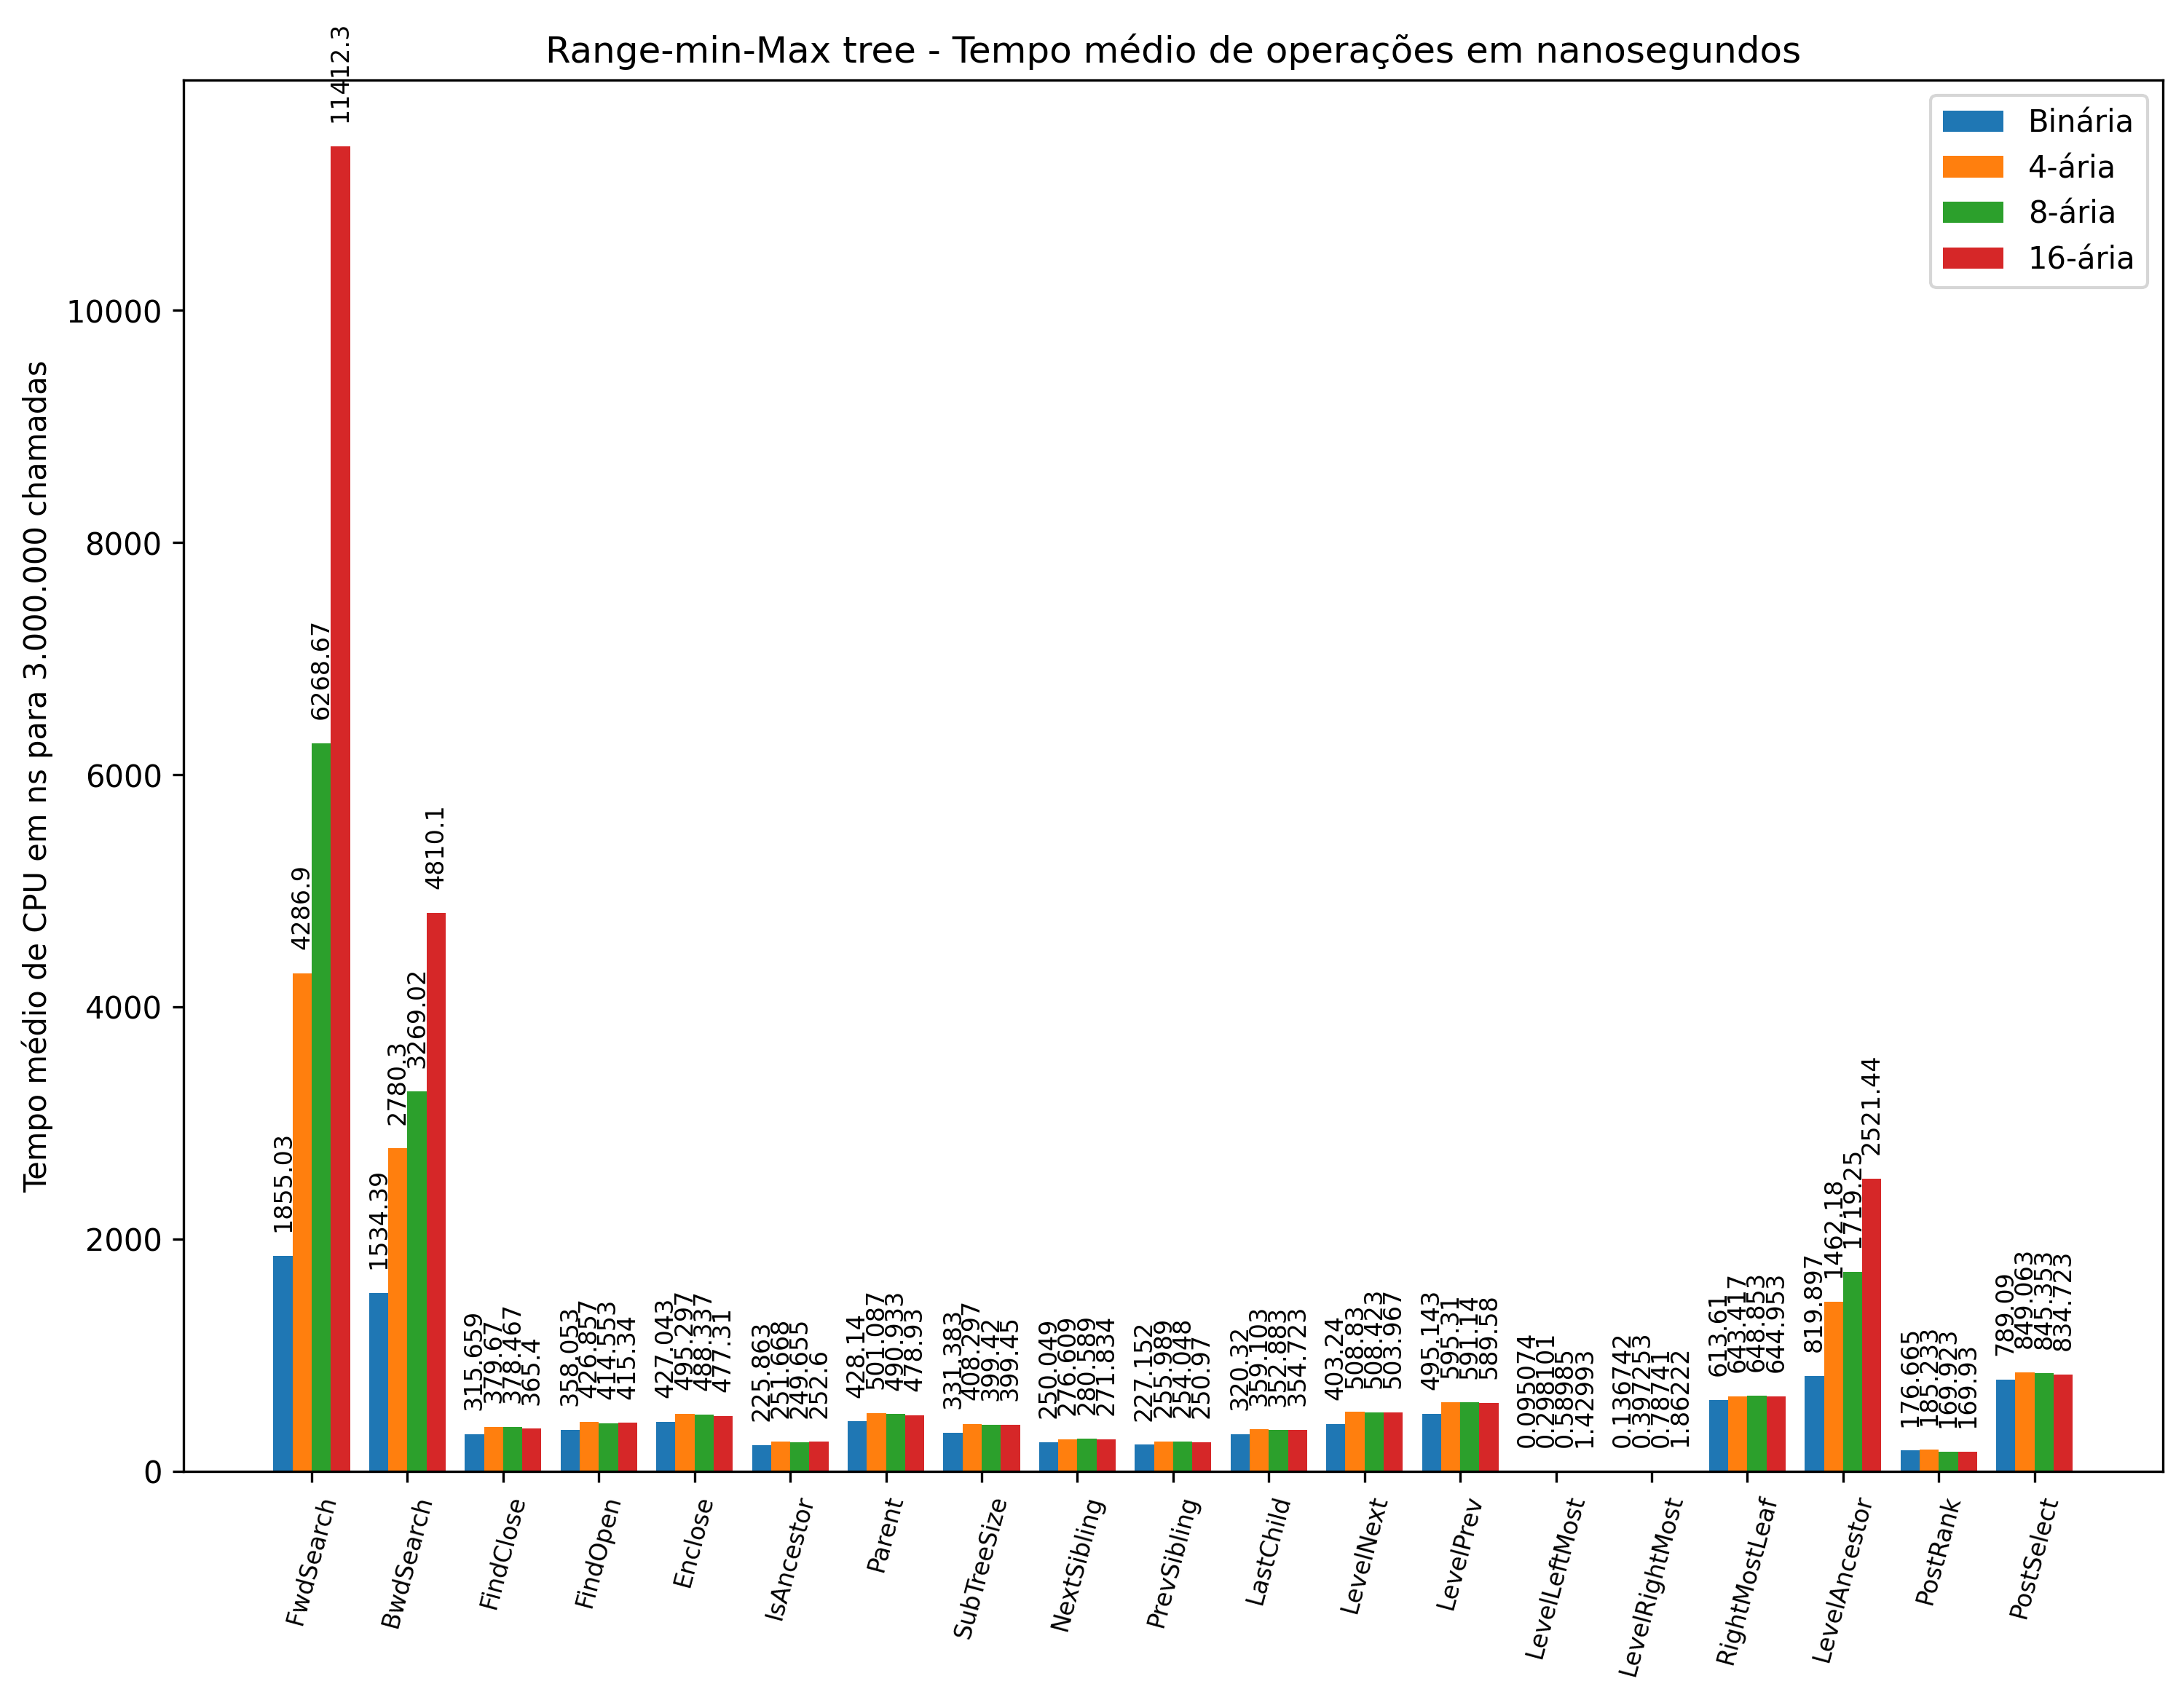
\includegraphics[scale=0.8, angle=270]{images/dna_i3000000.png}
        }
        \label{fig:dna}
\end{figure}

\begin{figure}[!ht]
    \centering
      \caption[Operações sobre o conjunto de dado proteins]{Tempo médio de operações sobre o conjunto Proteins}{
          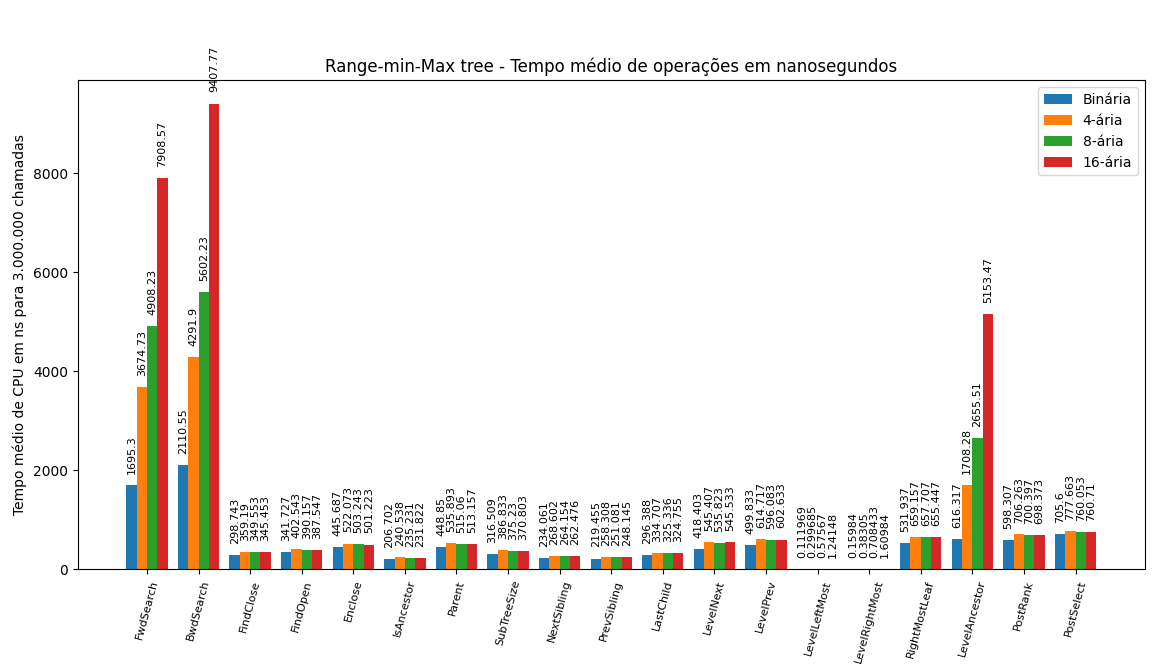
\includegraphics[scale=0.8, angle=270]{images/prot_i3000000.png}
        }
        \label{fig:prot}
\end{figure}

\begin{figure}[!ht]
    \centering
      \caption[Operações sobre o conjunto de dado wikipedia]{Tempo médio de operações sobre o conjunto Wikipedia}{
          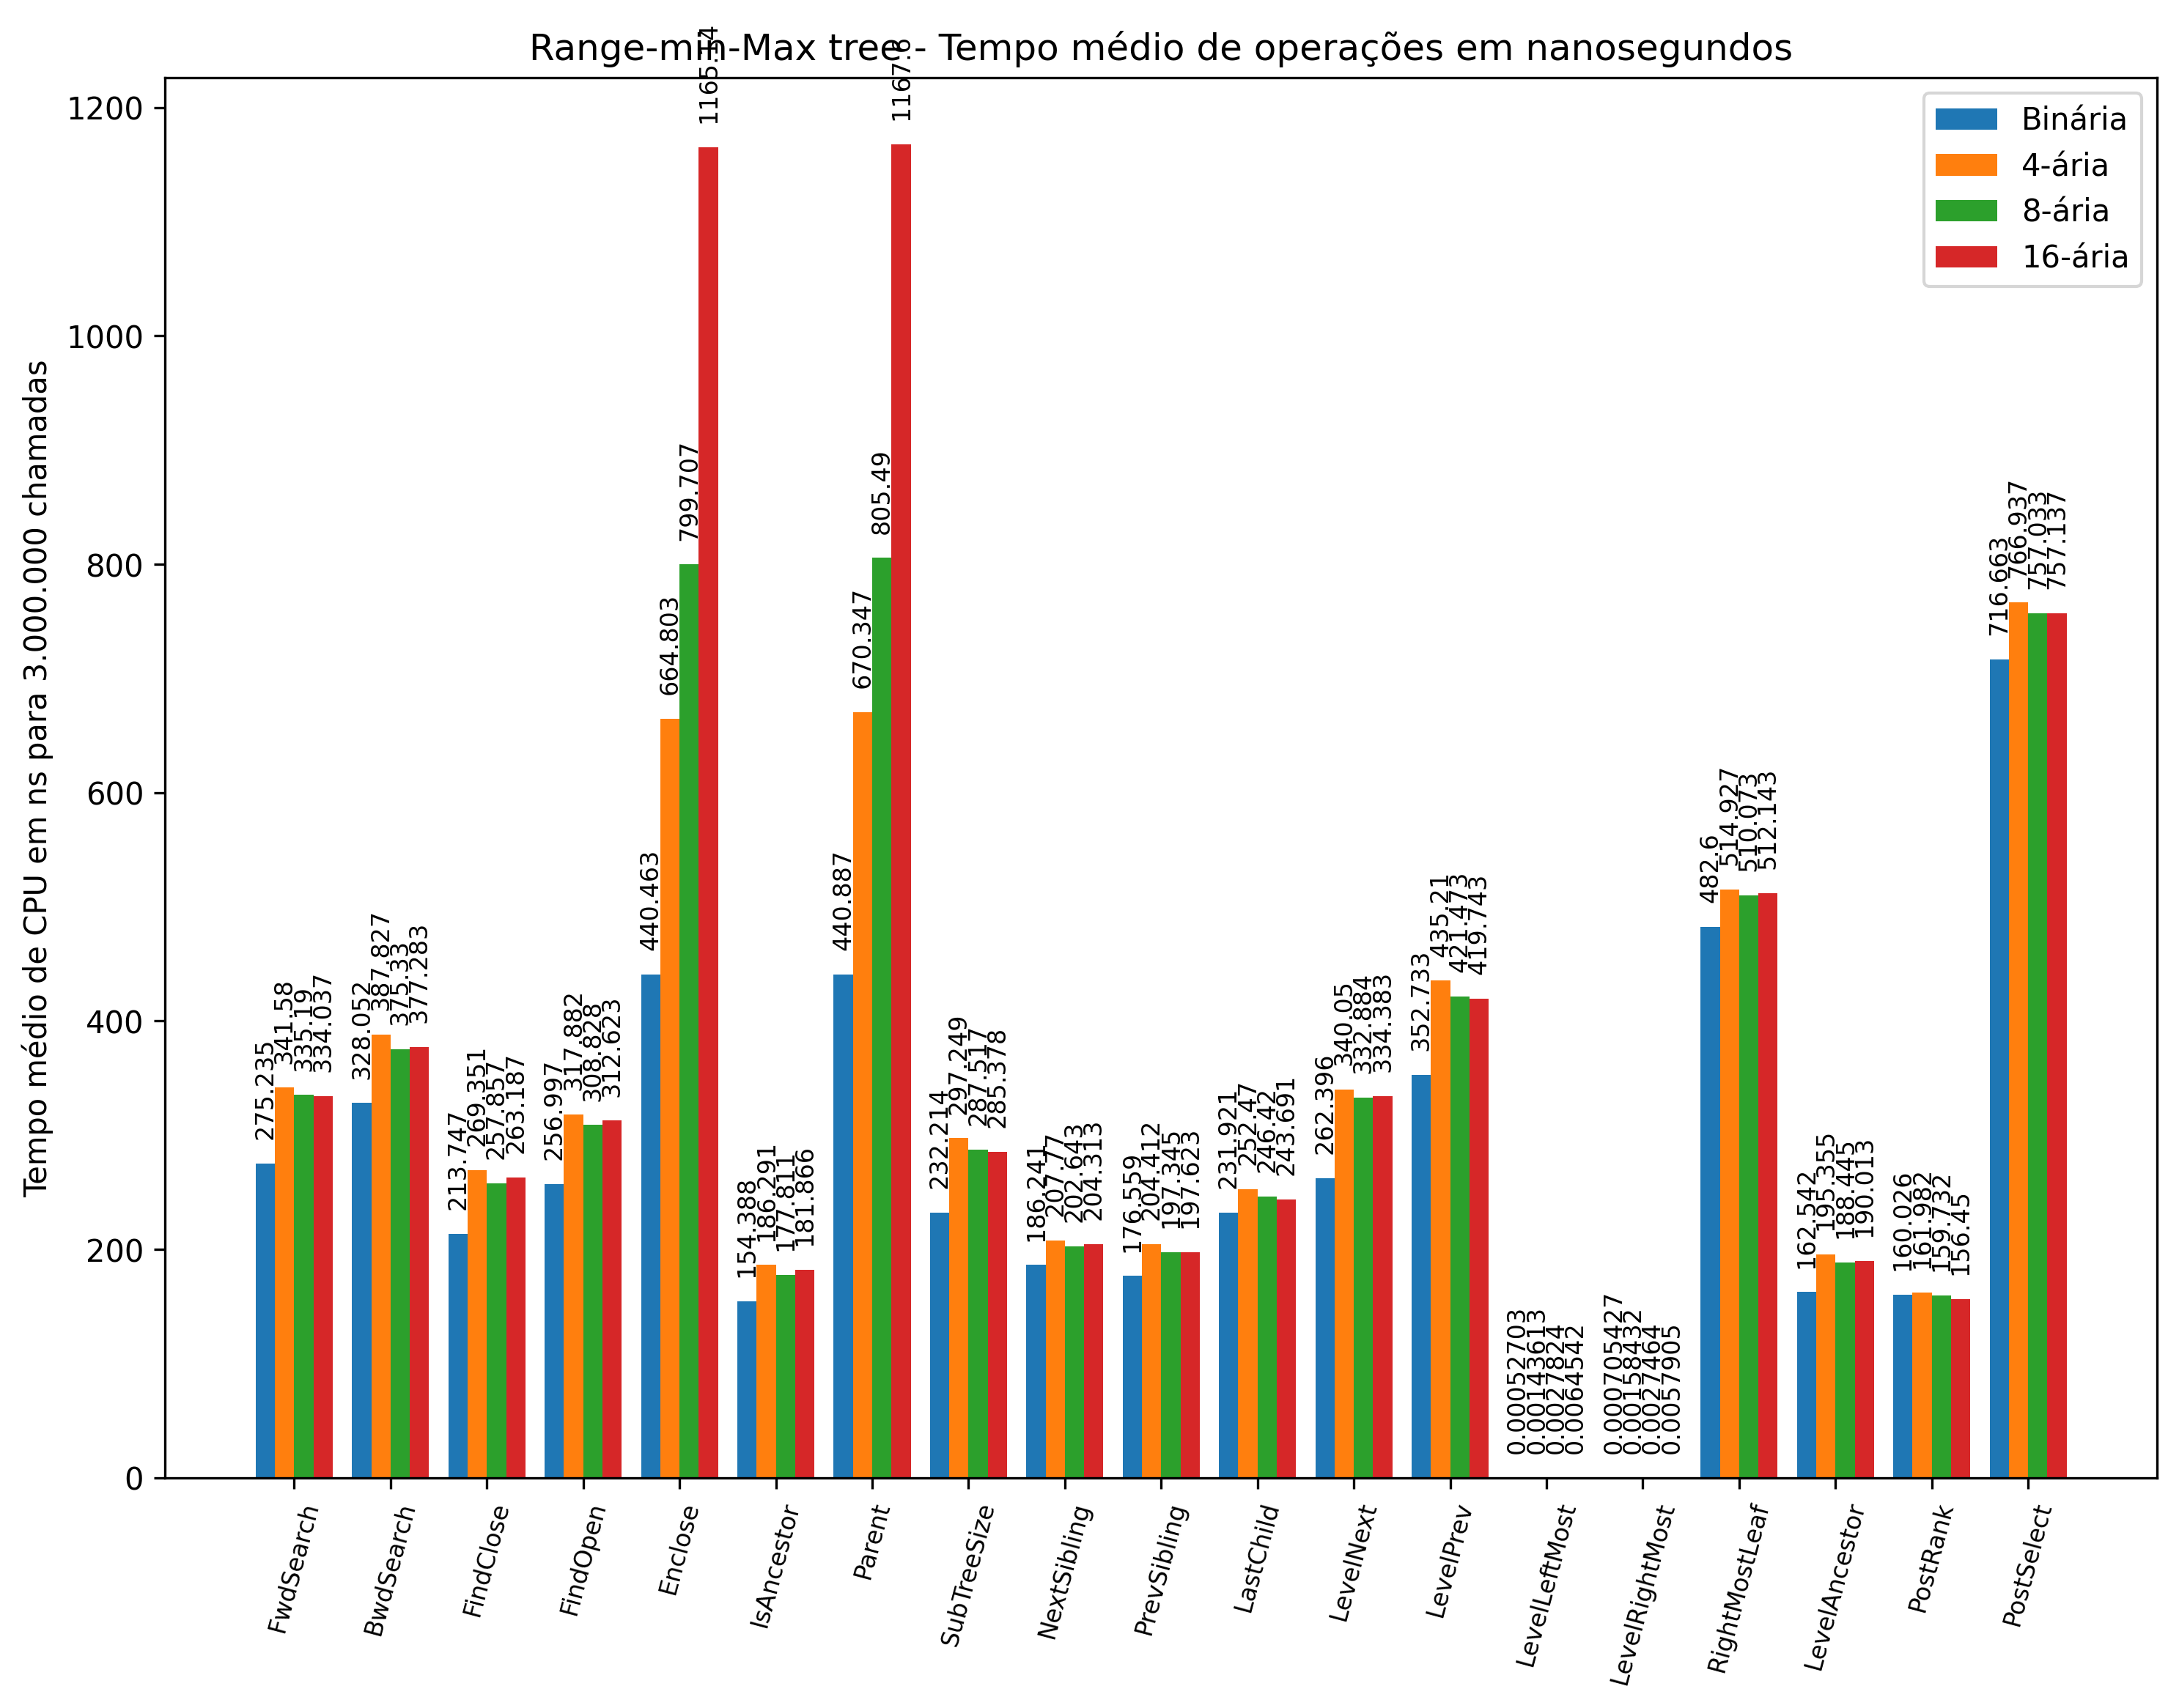
\includegraphics[scale=0.8, angle=270]{images/wiki_i3000000.png}
        }
        \label{fig:wiki}
\end{figure}
%base de dados, configuração, experimentos, resultados
%figura, resultado destacado.
  \chapter{Considerações Finais}\label{chp:conclusao}

Com o surgimento de novos dispositivos e o aumento na produção de dados, temos um grande desafio a superar, frente ao gargalo de comunicação existente entre memória e processador. Soluções como hierarquia de memória objetivam diminuir esse gargalo, entretanto quando se trabalha com uma alta quantidade de dados, estes tendem a ficar distribuídos entre os diferentes níveis de memória. Com isso o processador frequentemente precisa realizar buscas em memórias  nos níveis mais inferiores da hierarquia, o que acarreta em um acréscimo de tempo considerável no tempo de resposta, devido a alta latência dessas memórias.

As estruturas de dados sucintas possibilitam a representação e operaração sobre os seus objetos, usando espaço e tempo reduzido. Assim um dos objetivos deste trabalho era compreender e enfatizar a importância do estudo dessas estruturas. Entretanto, ao operar na memória principal, temos um novo gargalo de desempenho, dessa vez entre cache e memória principal, como mostram \citet{paper-making-btree-cache}, faz-se necessário então, buscarmos maneiras de melhor aproveitar a estrutura da memória cache. Uma das maneiras de fazer isso é tirando proveito da localidade espacial, maximizando o uso de uma linha de cache, que pode ser alcançada através da maximização do fator de ramificação destas estruturas. 

A rmM-tree é uma estrutura de dados sucinta que permite a navegação de forma eficiente em árvore através de valores de excesso máximos e mínimos em intervalos, porém a mesma é construída na forma de árvore binária, uma estrutura que possuí baixo fator de ramificação, e portanto baixo aproveitamento da linha de cache, nosso objetivo neste trabalho portanto era aumentar o fator de ramificação dessa estrutura, visando  melhor proveito da cache, como visto em \citep{paper-making-btree-cache}, o que reduziria significativamente o tempo gasto para realizar operações diversas. 

Implementamos e analisamos, para tanto, uma versão da rmM-tree de \citet{book-compact-data-structures}, e 3 versões de uma rmM-tree k-kária, compreendendo uma rmM-tree 4-ária, 8-ária, e uma rmM-tree 16-ária. De modo geral, os resultados obtidos a partir destas implementações não foram satisfatórios. Comparando a rmM-tree binária, frente às diferentes versões da rmM-tree k-ária, a primeira teve melhor desempenho em todas as operações. Em relação à rmM-tree k-ária, não foi possível detectar um padrão de comportamento para os diferentes conjuntos de dados usados nos testes. 

Para trabalhos futuros temos como objetivo reduzir o tempo das operações, através da otimização da implementação da rmM-tree k-ária. É necessário também melhorar o escopo dos nossos testes afim de monitorar de  modo mais claro e eficaz o uso da cache, o que envolve ampliar o escopo das ferramentas usadas. Sugere-se também investigar o impacto dessa proposta em diferentes ambientes, visando entender o efeito dessa estrutura diante de diferentes configurações de hardware. Por último temos como objetivo a implementação das demais operações de percurso em árvores suportadas pela range min-max tree clássica e que ainda não foram implementadas em sua versão k-ária. 

 
  \begin{references}
    %\bibliographystyle{plainnat}
    \bibliography{bib/references}
  \end{references}
  
 
\end{document}